\section{Event reconstruction and selection}
\label{sec:event_selection}

This section documents how particles are selected, how hadronic-event candidates are defined, and how data/MC agreement is validated at the particle-category level before unfolding. This validation is essential because the selected particles are the direct inputs to the thrust algorithm.

\subsection{Particle categories and \texttt{pwflag} mapping}

ALEPH reconstructed particles are categorized with an integer label \texttt{pwflag}. Table~\ref{tab:pwflag_definition} summarizes the categories used in this analysis.

\begin{table}[t!]
\centering
\begin{tabular}{c l}
\hline
\texttt{pwflag} & Category \\
\hline
0 & charged tracks \\
1 & charged leptons (tracker + ECAL category) \\
2 & charged leptons (tracker + muon category) \\
3 & $V^{0}$ candidates \\
4 & photons \\
5 & neutral hadrons \\
\hline
\end{tabular}
\caption{Particle-category labels used in archived ALEPH reconstructed events.}
\label{tab:pwflag_definition}
\end{table}

The archived reconstruction stores these objects as energy-flow candidates built from combined
tracking and calorimetric information. Charged categories are anchored by high-quality tracking
measurements, while neutral categories are anchored by calorimeter response. This object
representation is the direct input to thrust, so any category-dependent detector mismatch appears
as a potential migration effect in the unfolding response.

All selected charged and neutral categories contribute to the thrust numerator and denominator through their momentum vectors. Therefore, mismodeling in any category can bias the detector-level event-shape response and the unfolded result.

\subsection{Object-level and event-level selections}

Table~\ref{tab:particle_selection_summary} lists the object-level nominal selection with one requirement per row. These criteria define which reconstructed particles are propagated into thrust and therefore which detector effects enter the response model.

\begin{table}[t!]
\centering
\begin{tabular}{@{}p{0.37\textwidth}p{0.57\textwidth}@{}}
\hline
Selection item & Requirement \\
\hline
Charged category & \texttt{pwflag}\,$\in[0,2]$ \\
Charged acceptance & $|\cos\theta|\le 0.94$ \\
Charged transverse momentum & $p_{\mathrm{T}}\ge 0.2$ GeV \\
Charged impact parameter & $|d_0|\le 2$ cm \\
Charged longitudinal impact & $|z_0|\le 10$ cm \\
Charged hit quality & $N_{\mathrm{TPC}}\ge 4$ \\
Neutral category & \texttt{pwflag}\,$\in[3,5]$ \\
Neutral energy & $E\ge 0.4$ GeV \\
Neutral acceptance & $|\cos\theta|\le 0.98$ \\
Neutral hadron cleaning & reject \texttt{pwflag}=5 for $-0.19\le\cos\theta<-0.18$ \\
Use charged objects & \texttt{keepChargedTracks} = \texttt{True} (nominal) \\
Use neutral objects & \texttt{keepNeutralTracks} = \texttt{True} (nominal) \\
\hline
\end{tabular}
\caption{Object-level selections used to build the nominal thrust input particle set, with one line per requirement.}
\label{tab:particle_selection_summary}
\end{table}

The nominal hadronic event selection is summarized in Table~\ref{tab:event_selection_summary}, also with one line per requirement.

\begin{table}[t!]
\centering
\begin{tabular}{@{}p{0.37\textwidth}p{0.57\textwidth}@{}}
\hline
Selection item & Requirement \\
\hline
Ntuple preselection & \texttt{passesNTupleAfterCut} = 1 \\
Total charged energy & $E_{\mathrm{trk}}^{\mathrm{tot}}\ge 15$ GeV \\
Sphericity-axis acceptance & $|\cos\theta_{\mathrm{Sph}}|\le 0.82$ \\
Charged multiplicity & $N_{\mathrm{trk}}\ge 5$ \\
Total multiplicity & $N_{\mathrm{trk}}+N_{\mathrm{neu}}\ge 13$ \\
Visible energy guard & $E_{\mathrm{vis}}\ge 0$ GeV (nominally inactive) \\
Missing-momentum guard & $|\vec{p}_{\mathrm{miss}}|<9999$ GeV (nominally inactive) \\
\hline
\end{tabular}
\caption{Nominal event-level hadronic selection requirements, including guards present in code but inactive in the nominal configuration.}
\label{tab:event_selection_summary}
\end{table}

In practice, these selections enforce a phase space with high tracking quality, controlled forward
acceptance, and stable visible-energy topology before entering event-shape reconstruction. They are
chosen to follow ALEPH-standard hadronic selections while retaining explicit control over the
regions that dominate event-shape sensitivity.

The neutral hadron cleaning requirement (reject \texttt{pwflag}=5 for $-0.19\le\cos\theta<-0.18$) removes a localized region where the ALEPH hadronic calorimeter response is known to produce spurious neutral-hadron candidates. This narrow angular window corresponds to a structural gap in the detector and was identified from the data/MC neutral-hadron $\cos\theta$ distribution.

$V^0$ candidates (\texttt{pwflag}=3) include $K_S$ and $\Lambda$ from displaced-vertex reconstruction. These objects enter the thrust sum with their measured momentum vector rather than individual decay products, which is consistent with treating them as single hadronic objects for event-shape purposes. Their contribution to the thrust numerator and denominator is captured by the neutral-response systematic variations.

\subsection{Particle-category kinematic validation}

Before constructing thrust-family observables, we validate the reconstructed particle-level
ingredients that enter the event-shape sums and axis determination. Any mismodeling in particle
acceptance, momentum scale, or category composition can propagate into migration in the detector
response matrix and into unfolded distributions. To assess detector modeling of these inputs, we
compare data and MC reco distributions for each \texttt{pwflag} category using Data/MC ratio
panels, with generator-level references from \texttt{tgen} and \texttt{tgenBefore}. These
validation plots are taken from the dedicated validation snapshot with the same nominal selection
configuration used for the current thrust workflow.

\noindent
Figures~\ref{fig:pwflag0_full}--\ref{fig:pwflag5_full} provide the full variable-by-variable
checks for each reconstructed particle category that contributes to thrust. In each case, the
same observable set is shown to keep the detector-level validation uniform across categories:
angular acceptance, momentum scale, and quality-related variables are all checked before
constructing event-shape observables.

\begin{figure}[t!]
\centering
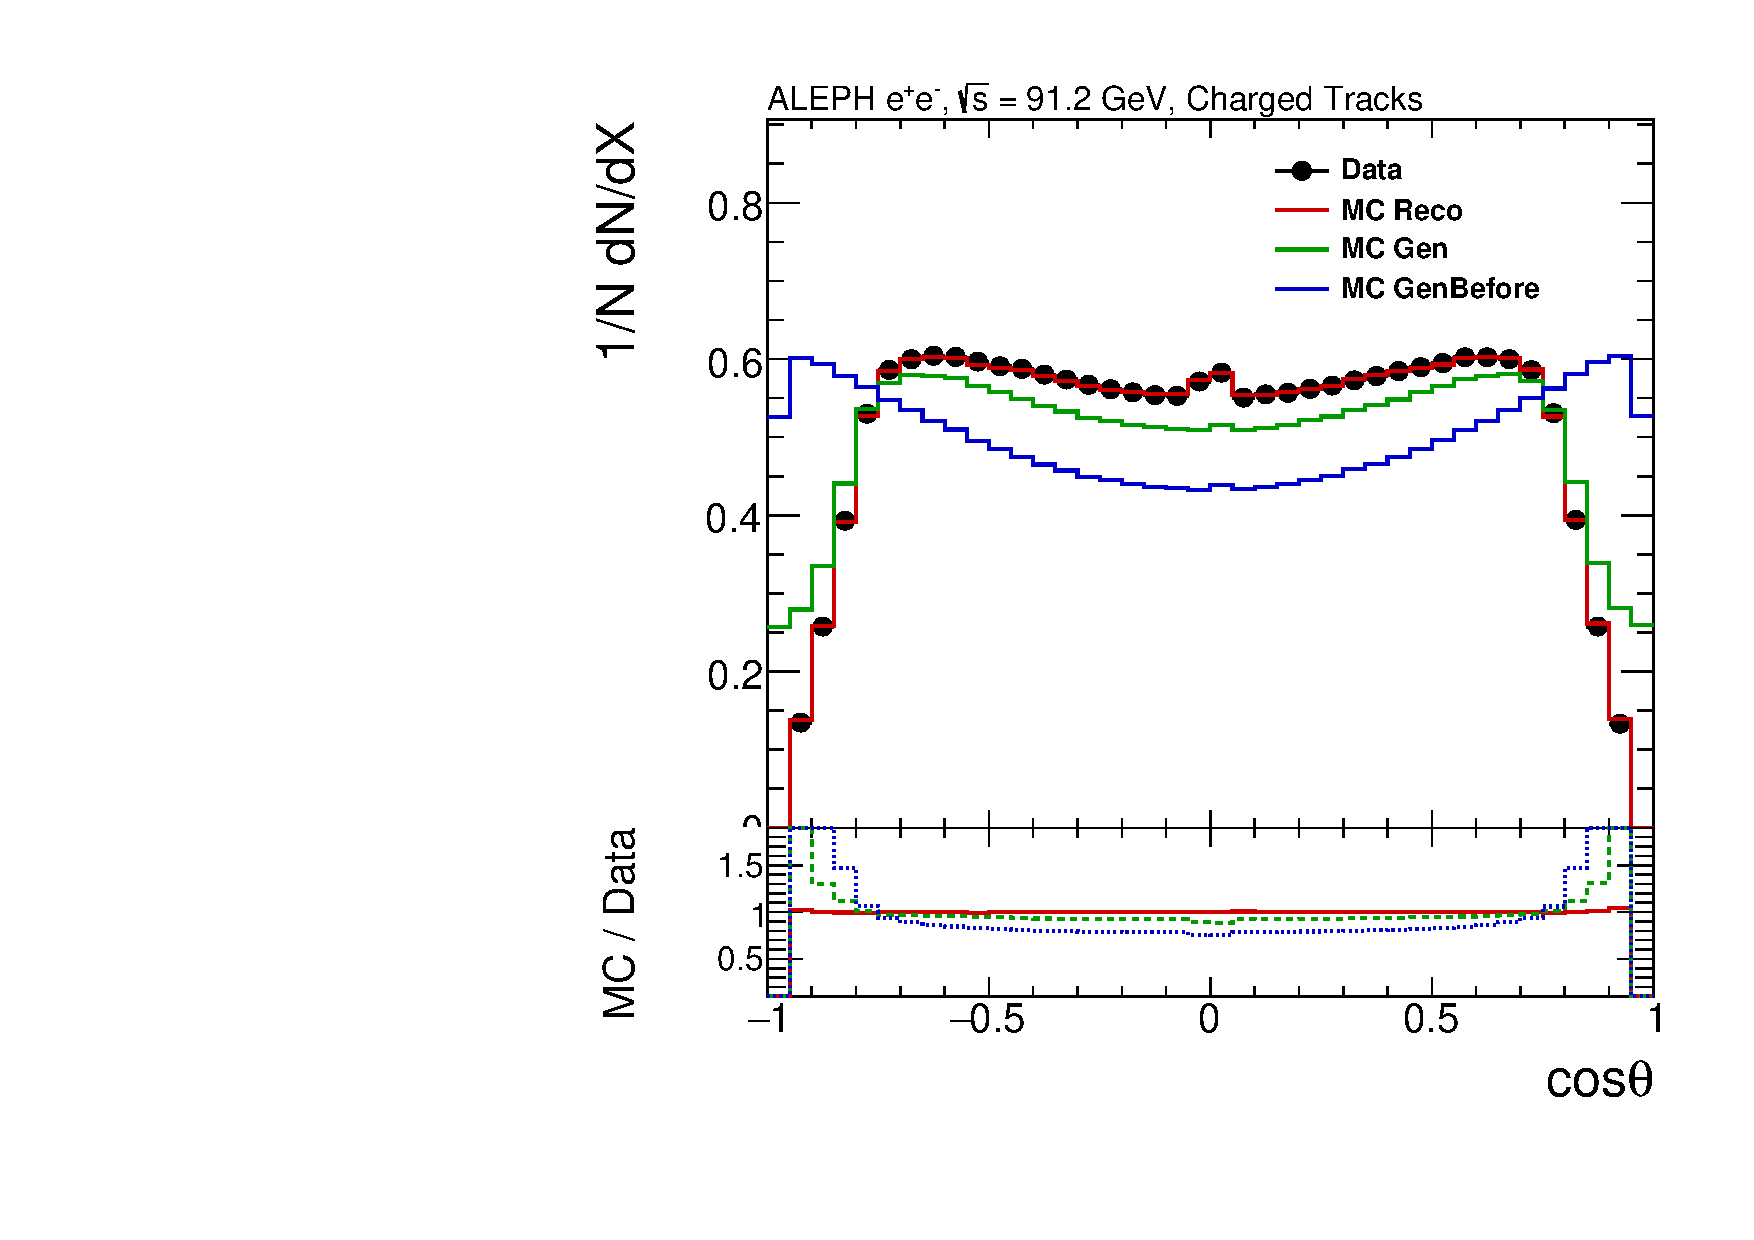
\includegraphics[width=0.325\textwidth]{../Studies/PreliminaryResult/2026-02-17_thrust_iter5/pwflag_kinematics/pwflag0_cosTheta.pdf}
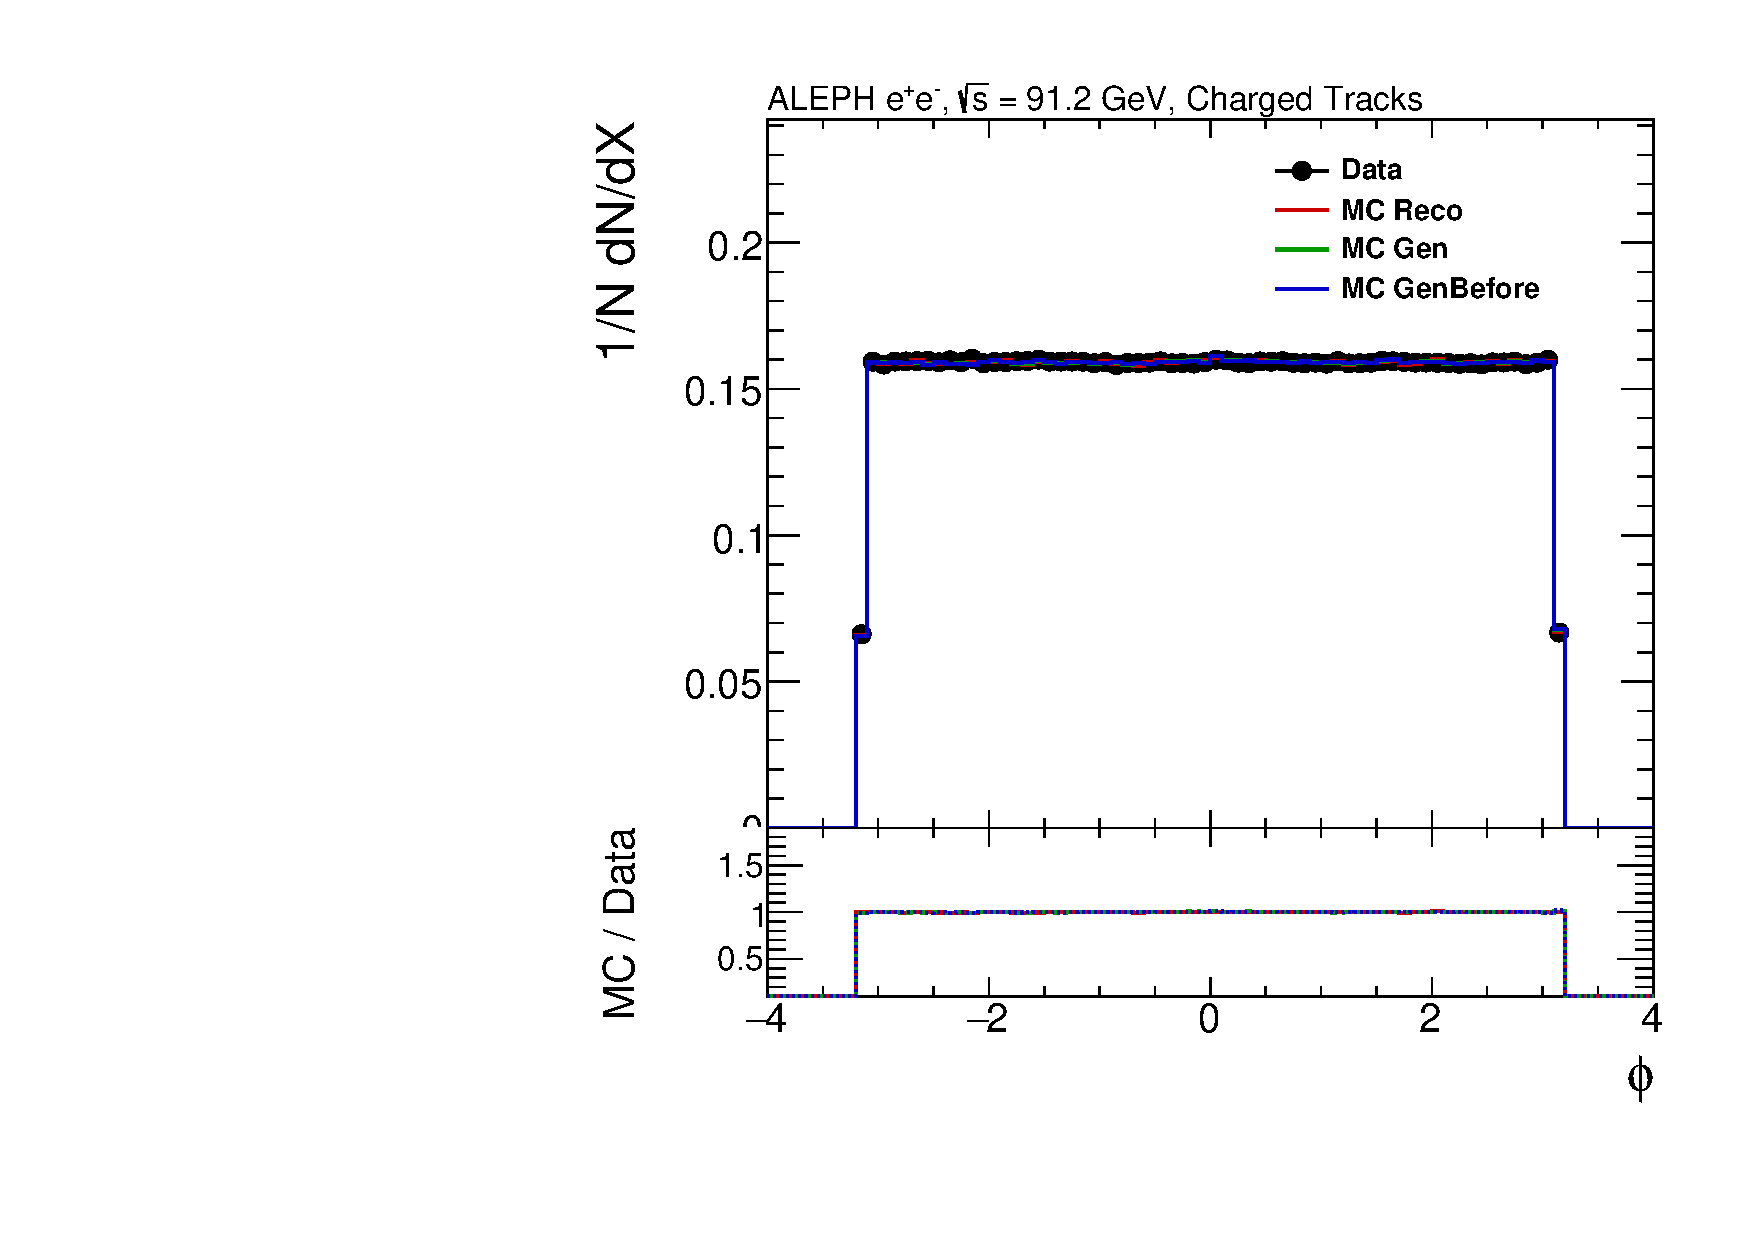
\includegraphics[width=0.325\textwidth]{../Studies/PreliminaryResult/2026-02-17_thrust_iter5/pwflag_kinematics/pwflag0_phi.pdf}
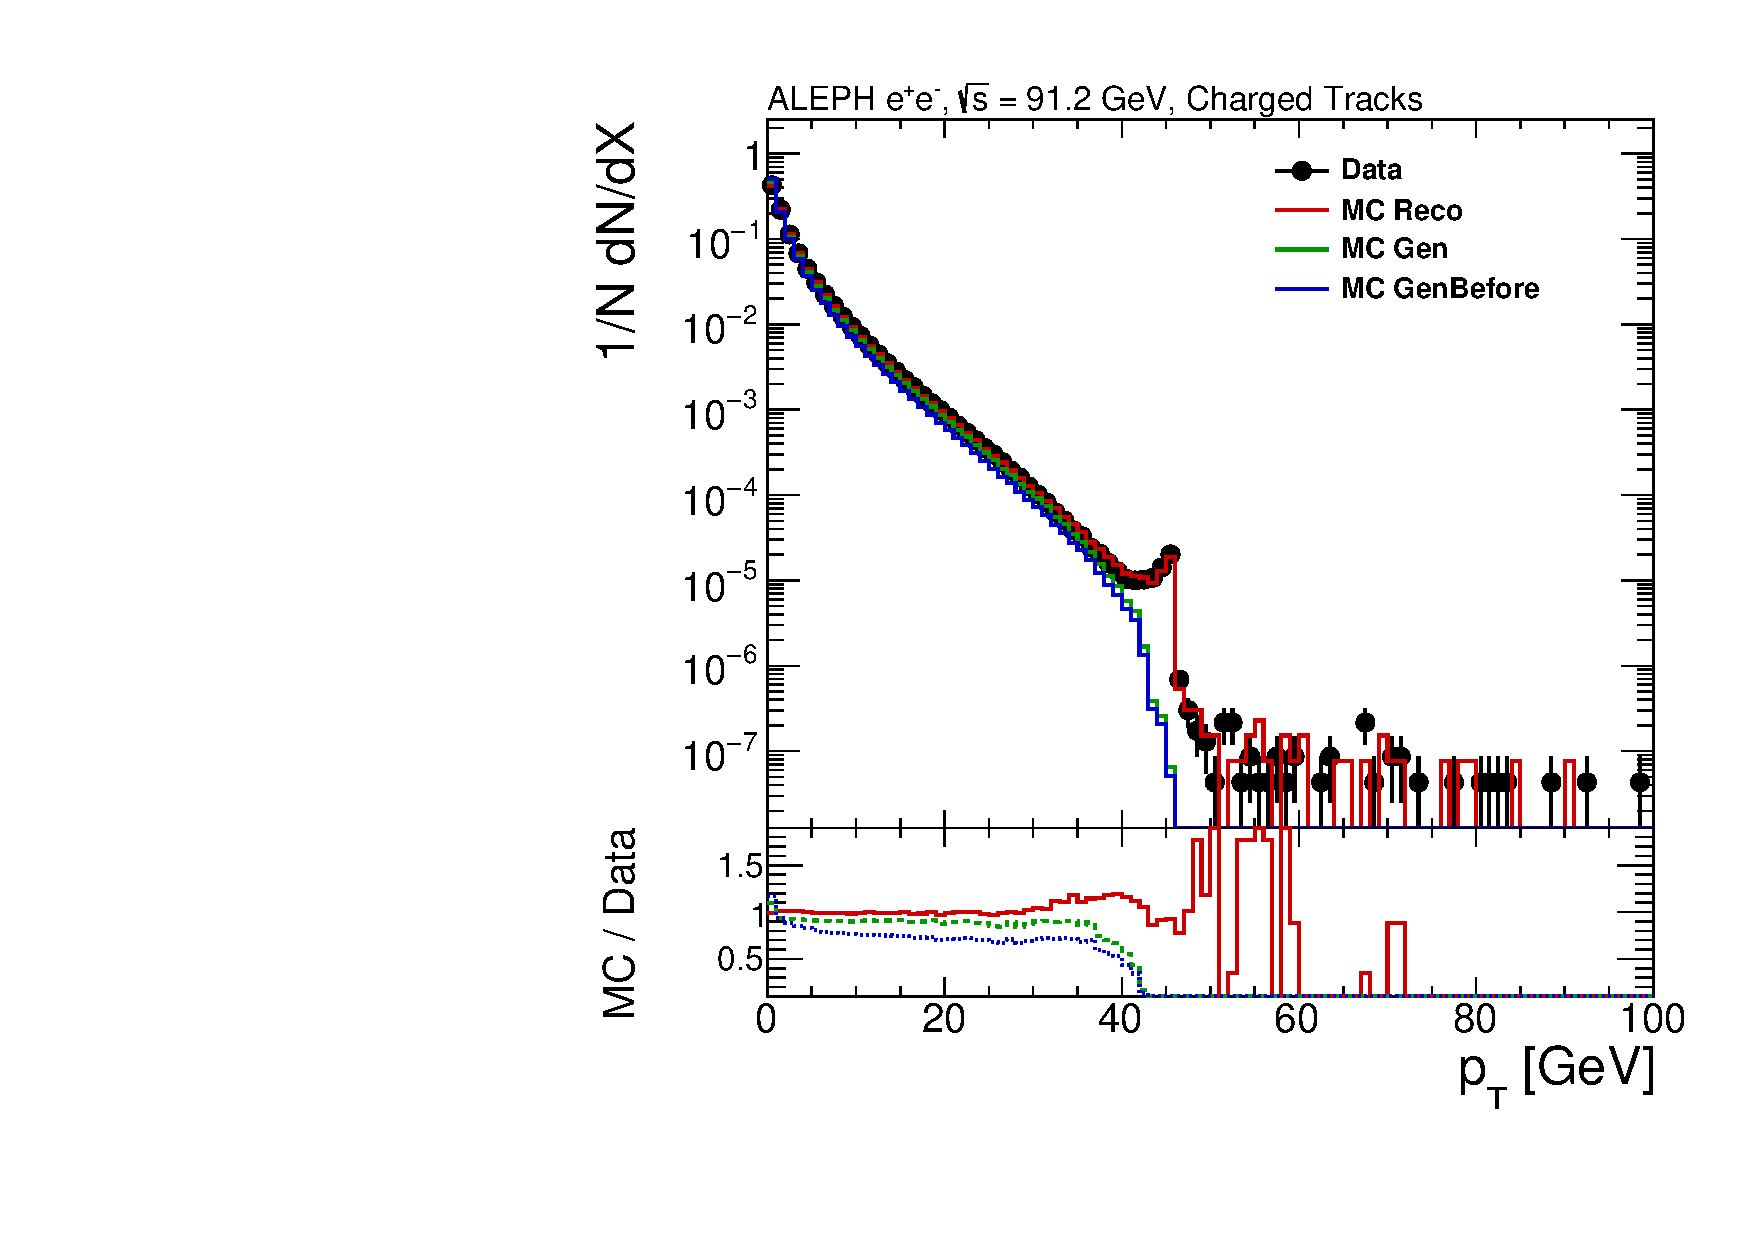
\includegraphics[width=0.325\textwidth]{../Studies/PreliminaryResult/2026-02-17_thrust_iter5/pwflag_kinematics/pwflag0_pt.pdf}
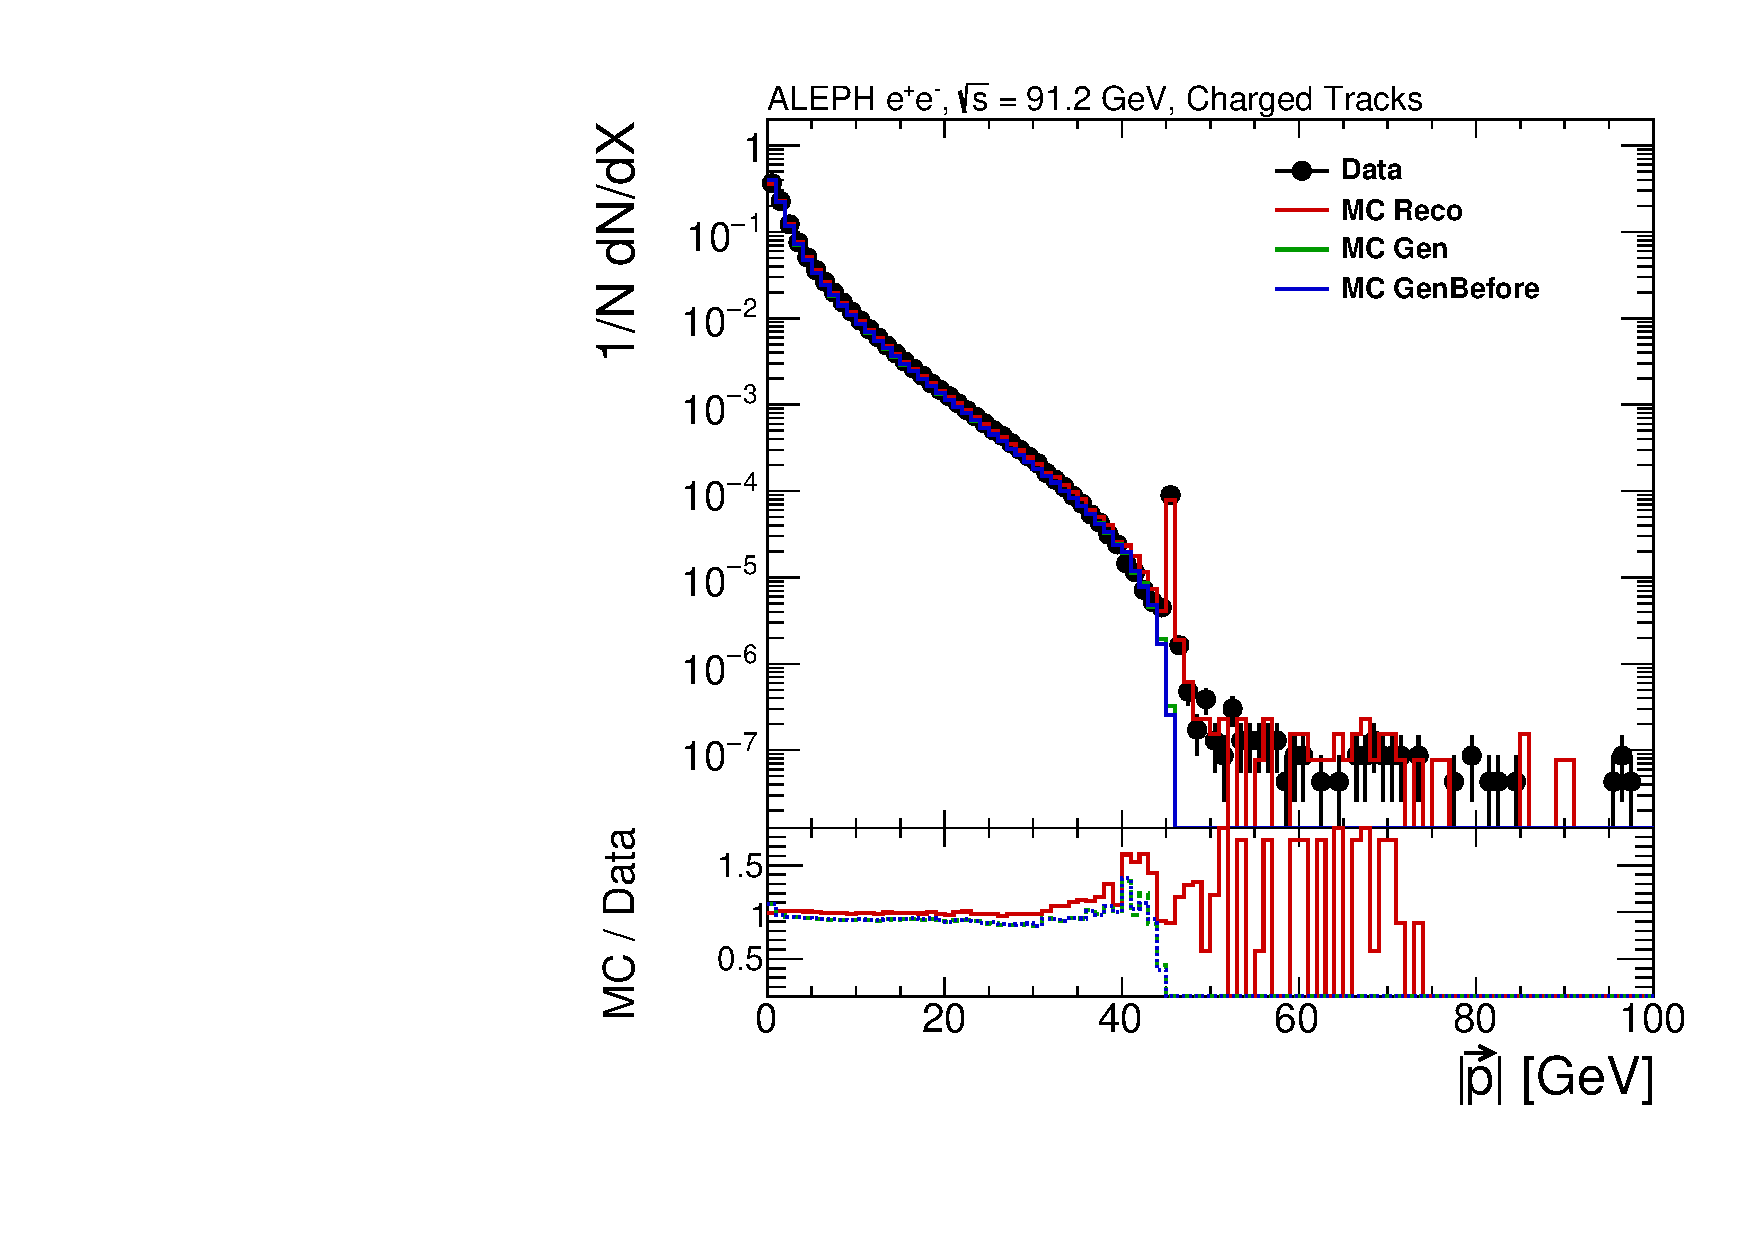
\includegraphics[width=0.325\textwidth]{../Studies/PreliminaryResult/2026-02-17_thrust_iter5/pwflag_kinematics/pwflag0_pmag.pdf}
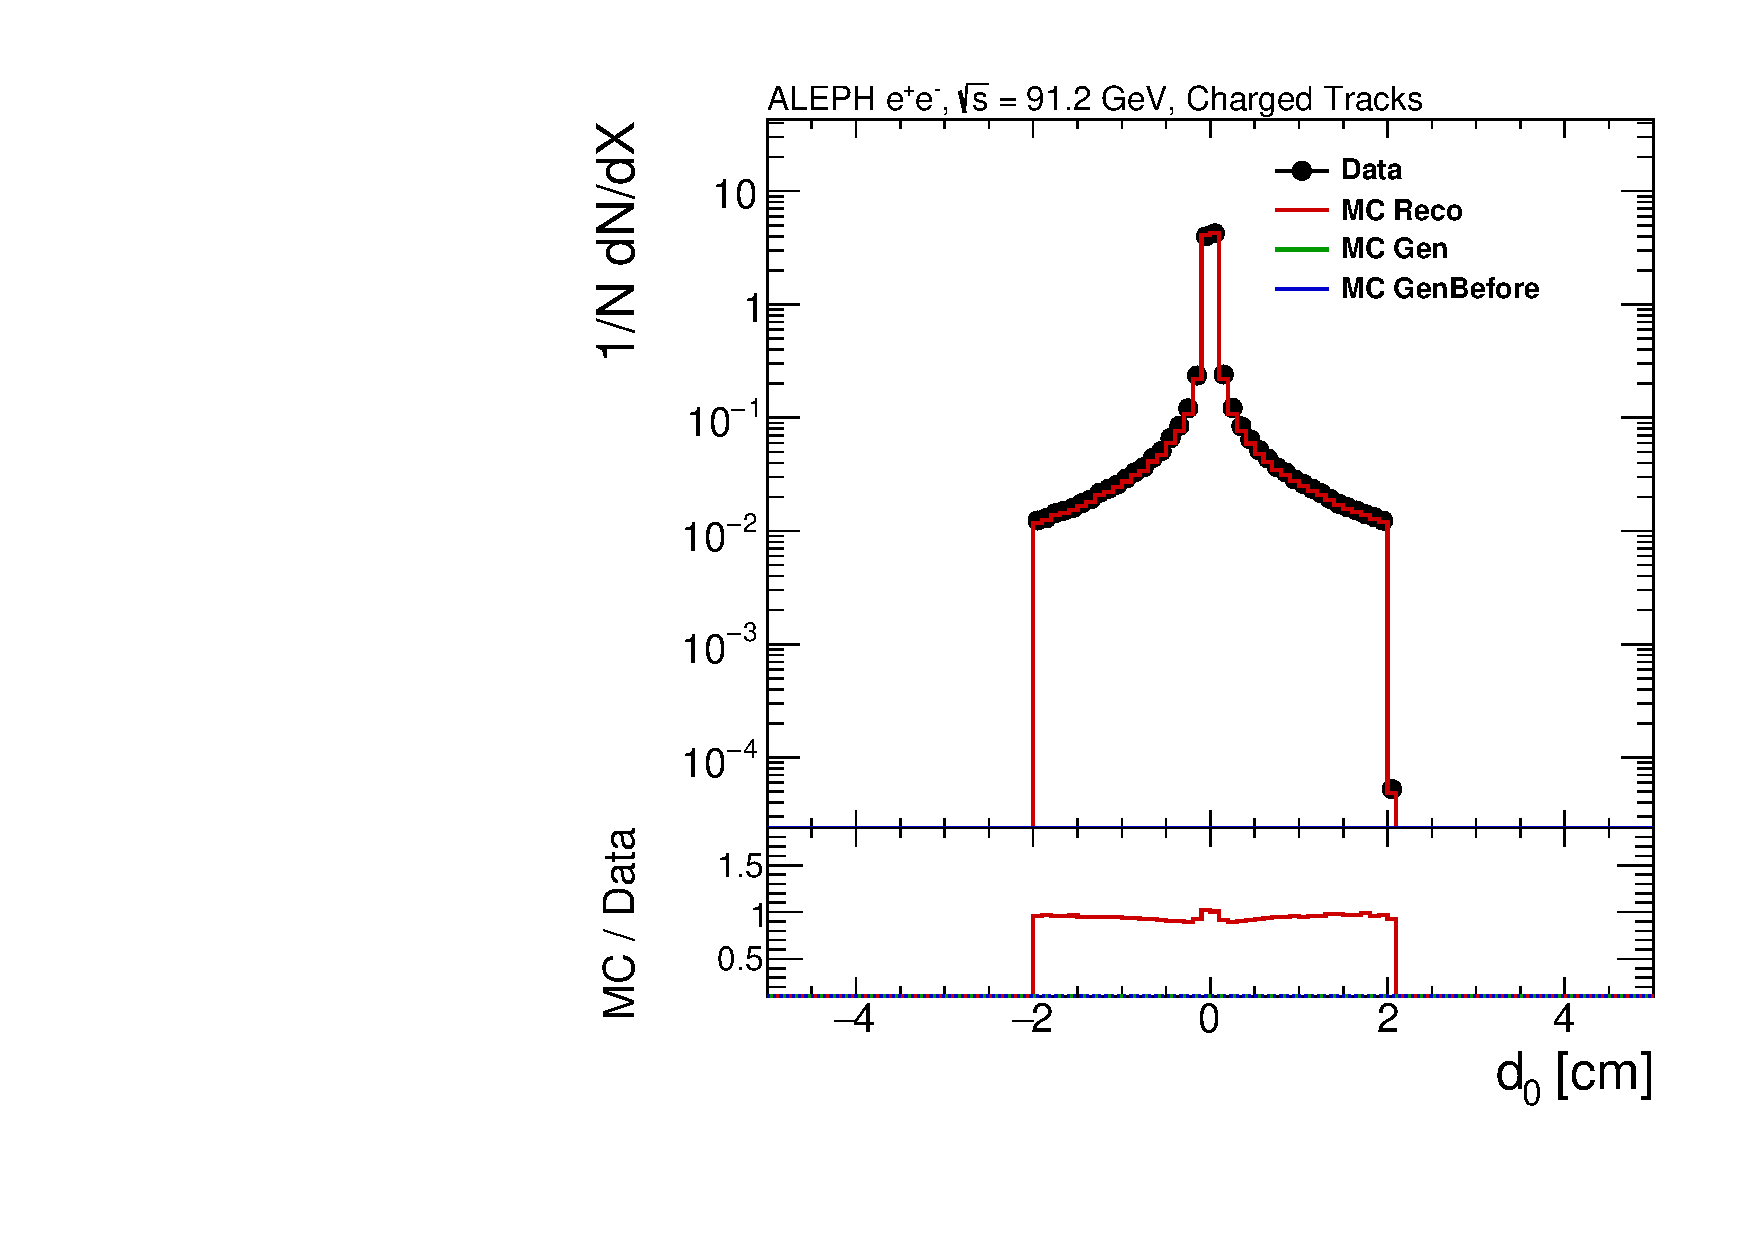
\includegraphics[width=0.325\textwidth]{../Studies/PreliminaryResult/2026-02-17_thrust_iter5/pwflag_kinematics/pwflag0_d0.pdf}
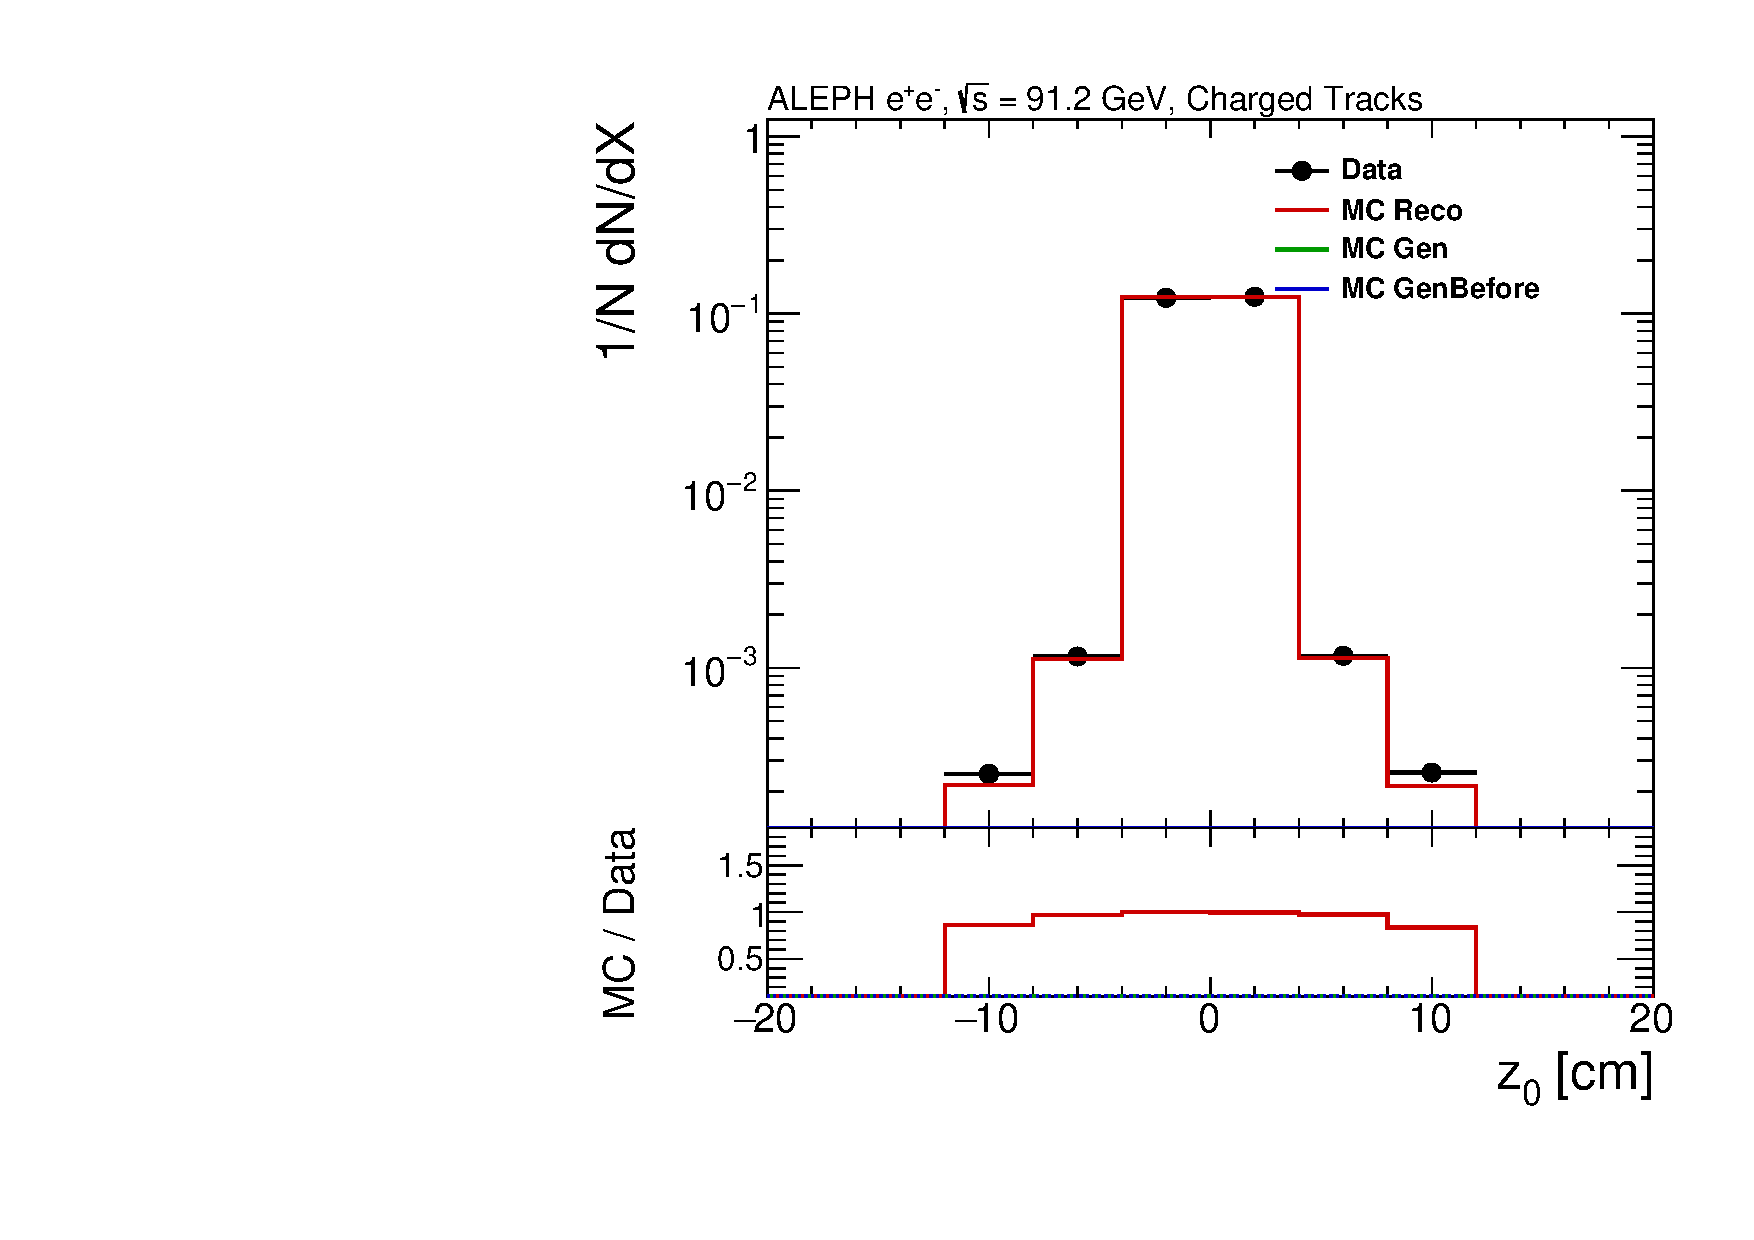
\includegraphics[width=0.325\textwidth]{../Studies/PreliminaryResult/2026-02-17_thrust_iter5/pwflag_kinematics/pwflag0_z0.pdf}
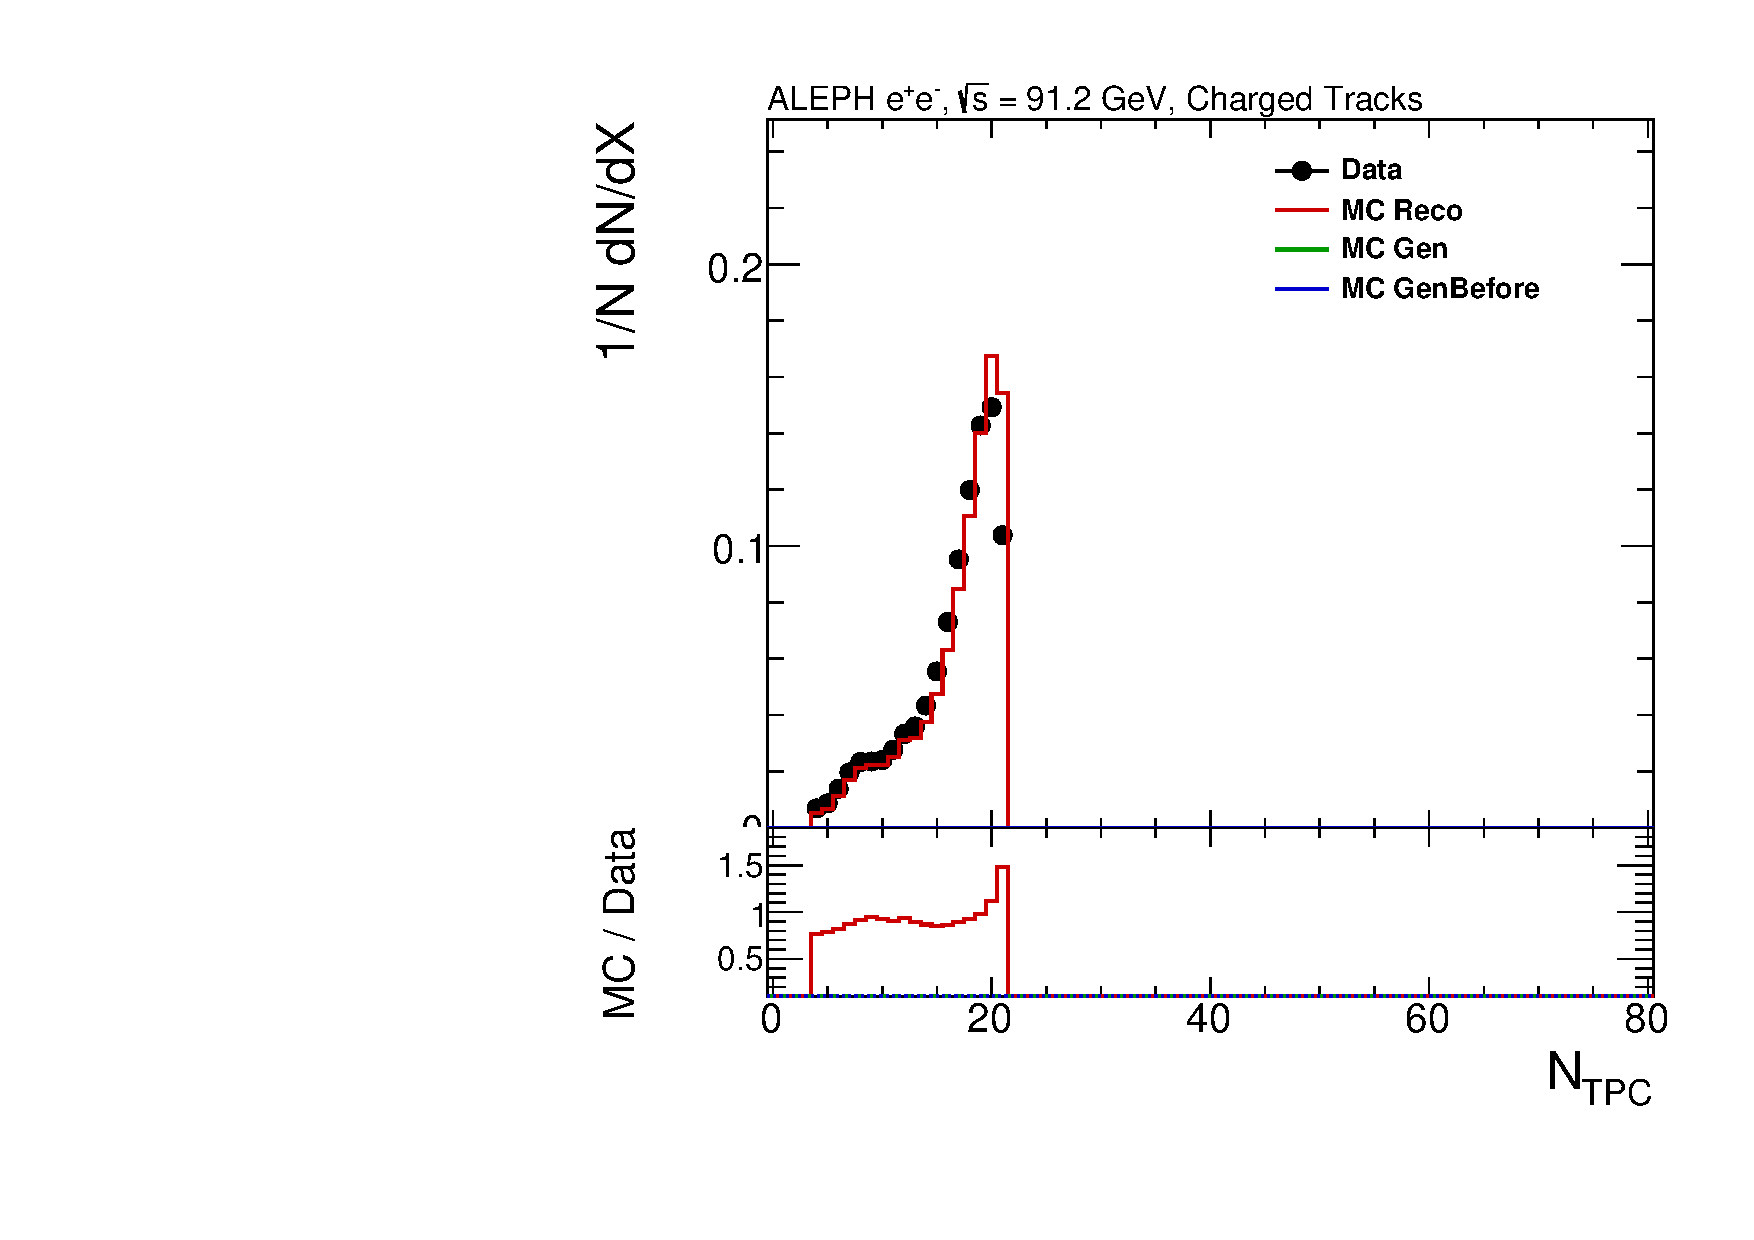
\includegraphics[width=0.325\textwidth]{../Studies/PreliminaryResult/2026-02-17_thrust_iter5/pwflag_kinematics/pwflag0_ntpc.pdf}
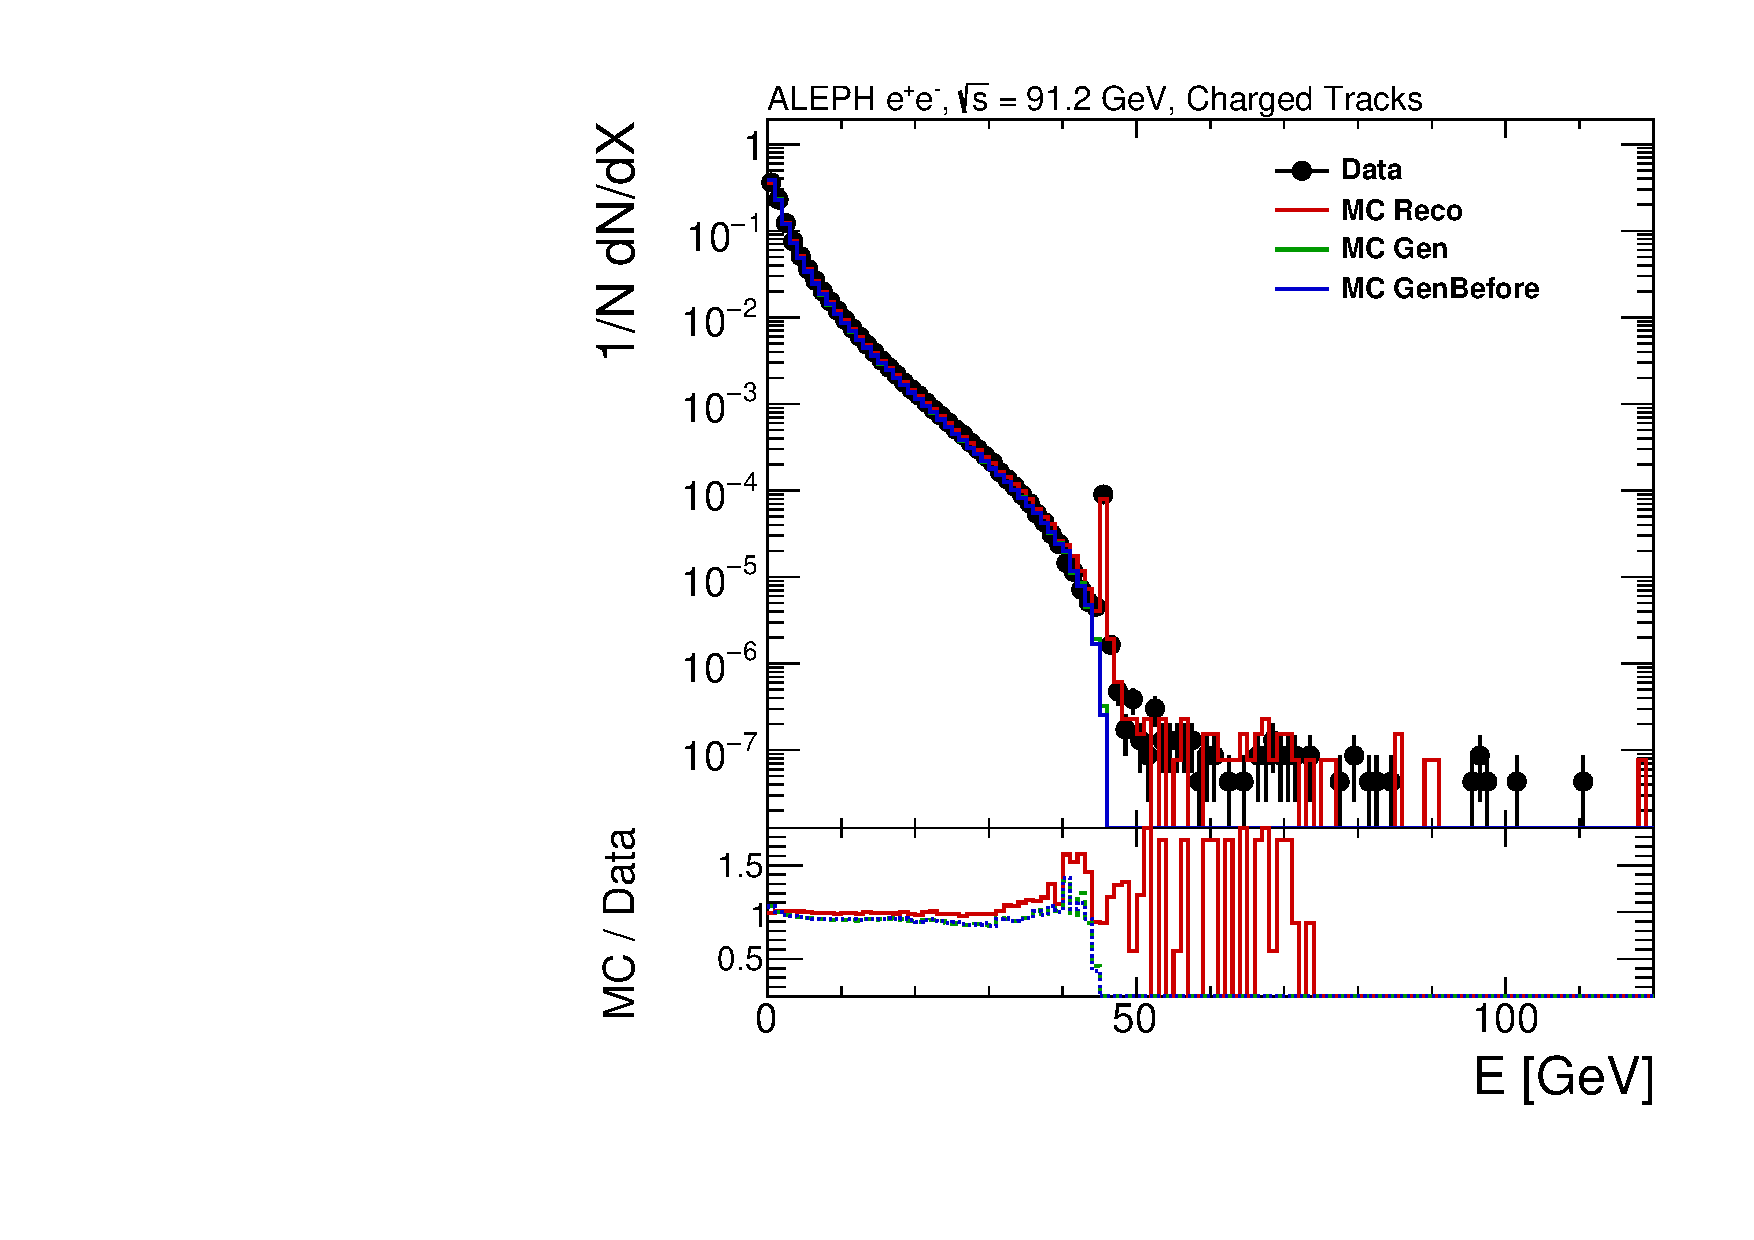
\includegraphics[width=0.325\textwidth]{../Studies/PreliminaryResult/2026-02-17_thrust_iter5/pwflag_kinematics/pwflag0_energy.pdf}
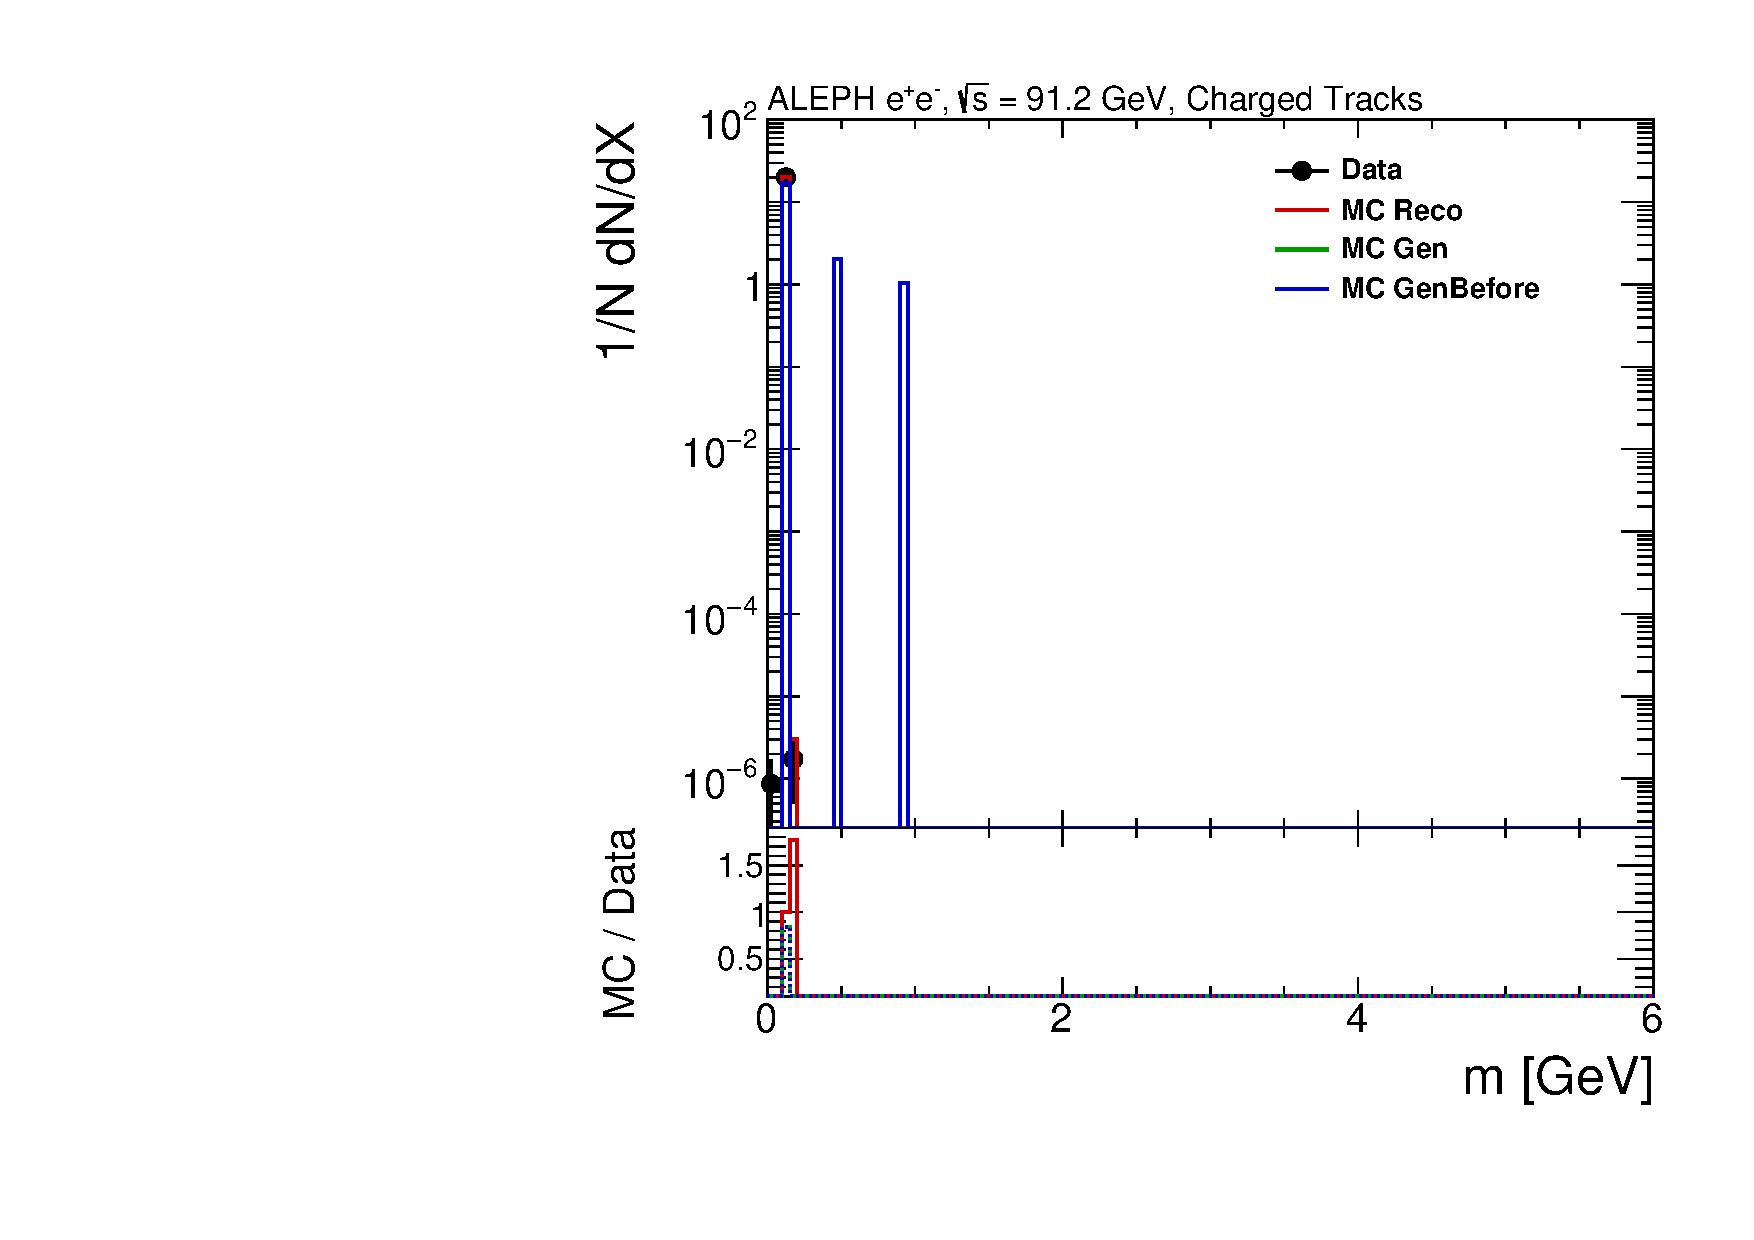
\includegraphics[width=0.325\textwidth]{../Studies/PreliminaryResult/2026-02-17_thrust_iter5/pwflag_kinematics/pwflag0_mass.pdf}
\caption{Complete \texttt{pwflag}=0 kinematic set.}
\label{fig:pwflag0_full}
\end{figure}

\noindent
In Fig.~\ref{fig:pwflag0_full}, the charged-track category drives the event-shape denominator
and axis finding, so agreement here anchors the full detector response modeling. The
$\cos\theta$ distribution shows the expected enhancement away from the acceptance edges and a
falloff near the fiducial boundary, while the $d_0$ and $z_0$ spectra are concentrated in the
high-quality track region selected for the nominal sample. The $N_{\mathrm{TPC}}$, $p_T$, and
energy panels provide direct checks that tracking-quality and hard-track tails are described with
the precision required for stable thrust unfolding.

\begin{figure}[t!]
\centering
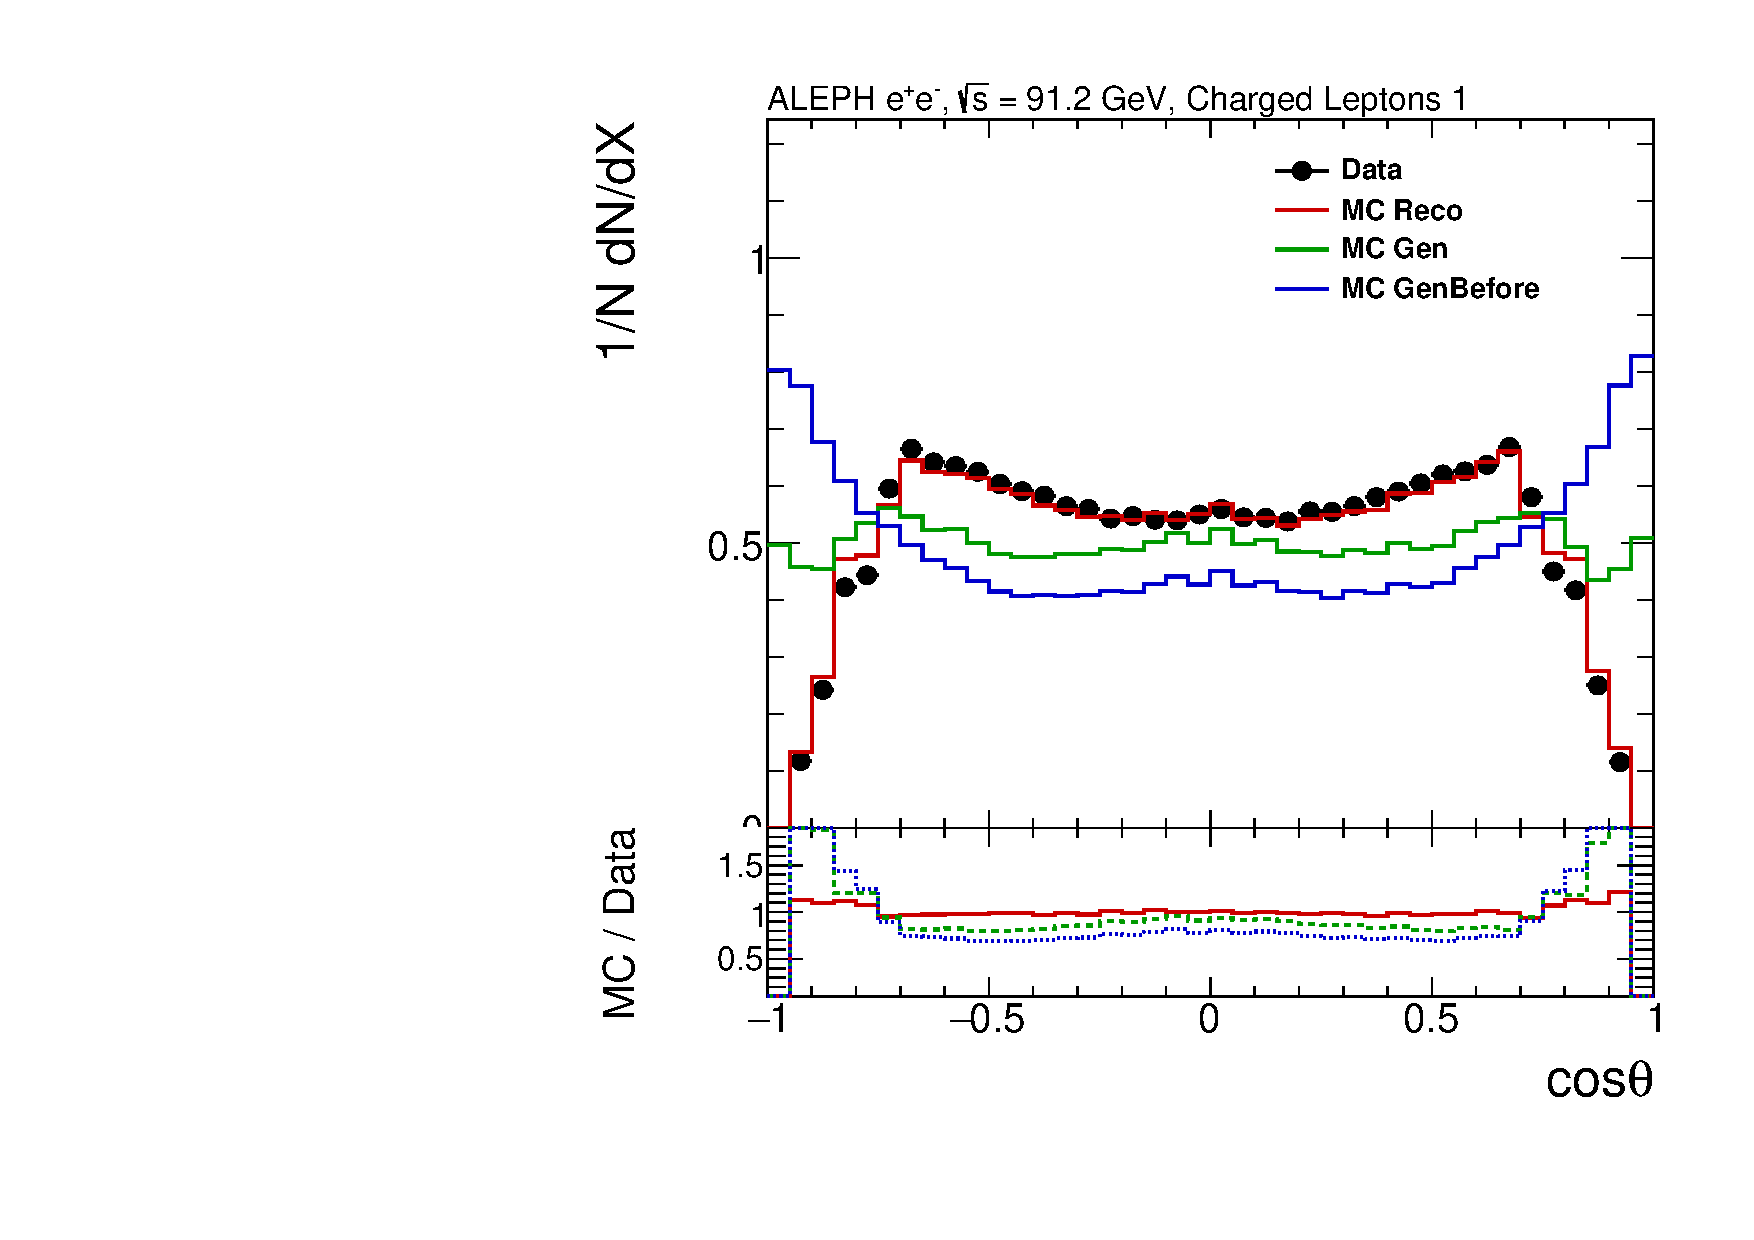
\includegraphics[width=0.325\textwidth]{../Studies/PreliminaryResult/2026-02-17_thrust_iter5/pwflag_kinematics/pwflag1_cosTheta.pdf}
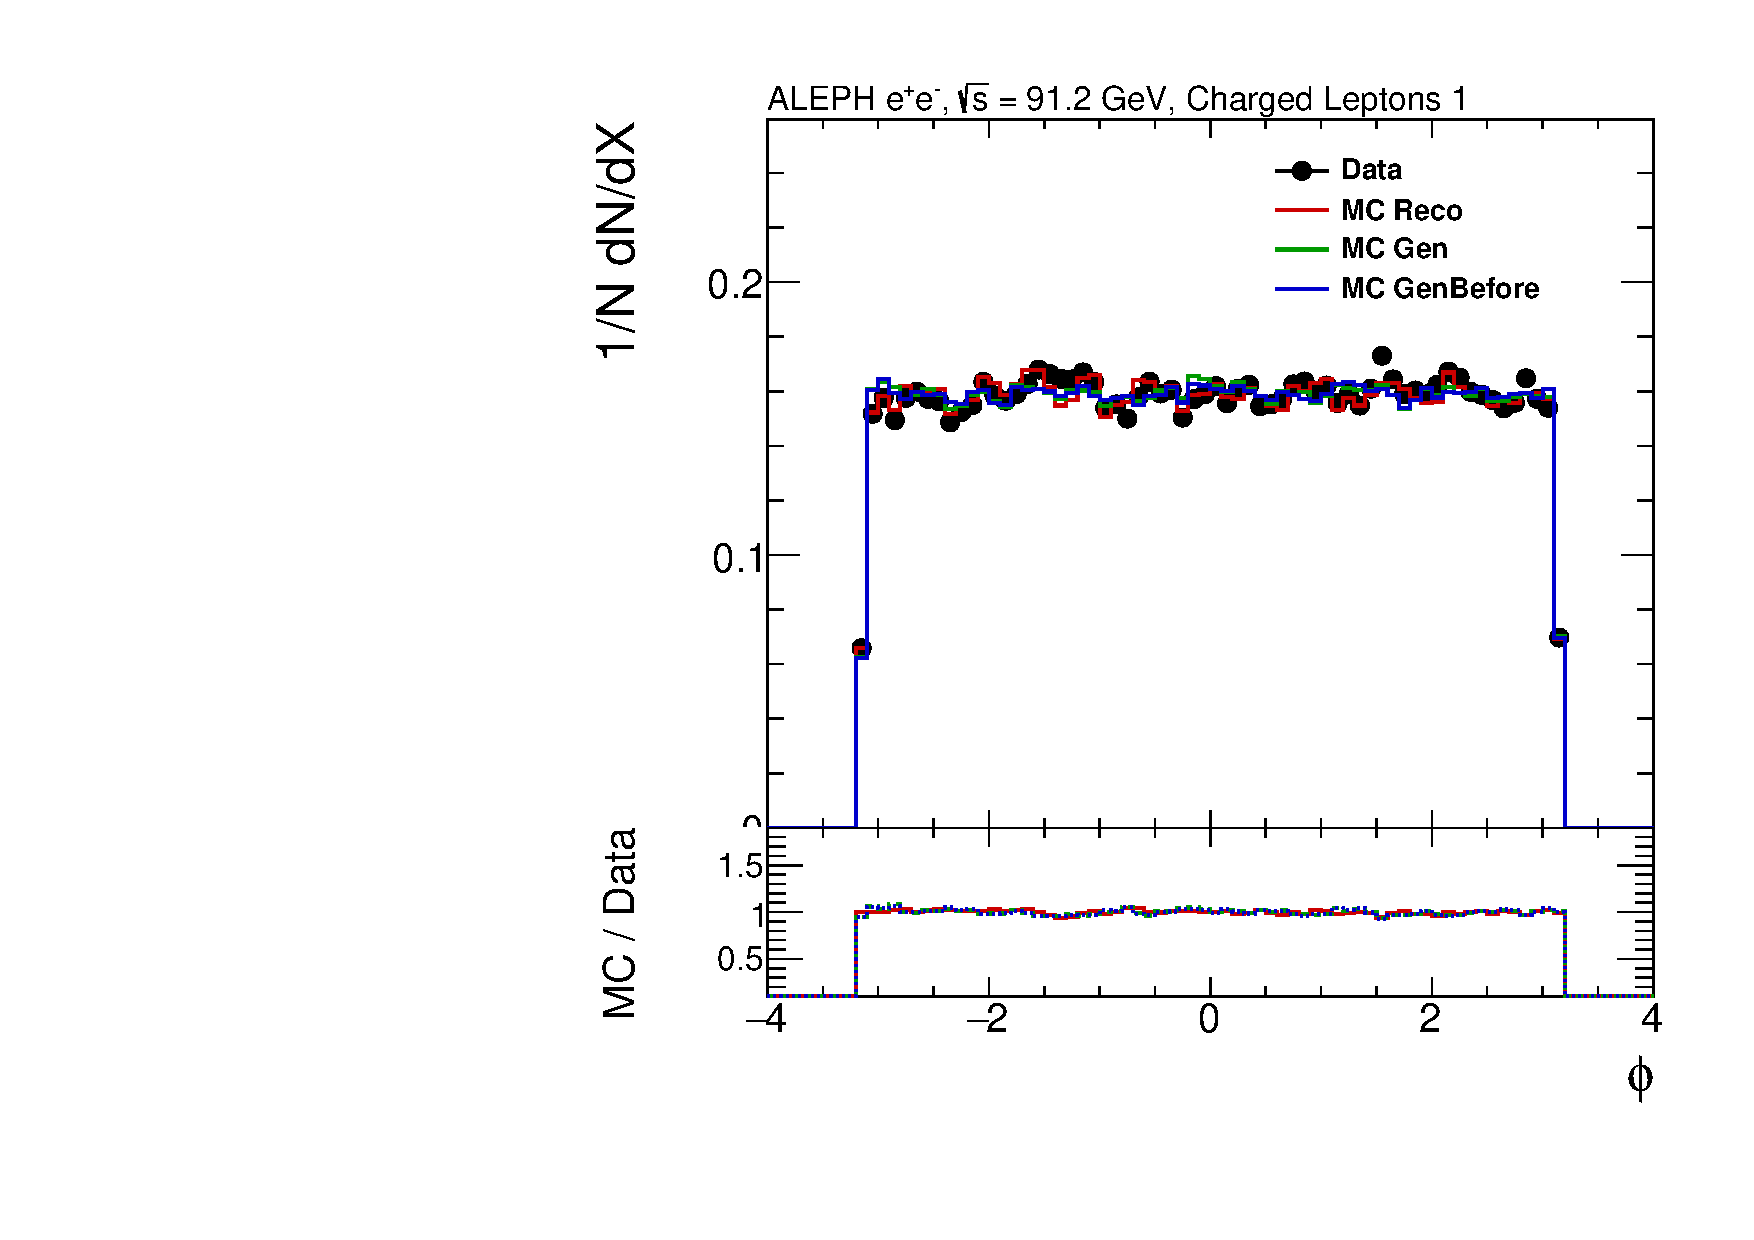
\includegraphics[width=0.325\textwidth]{../Studies/PreliminaryResult/2026-02-17_thrust_iter5/pwflag_kinematics/pwflag1_phi.pdf}
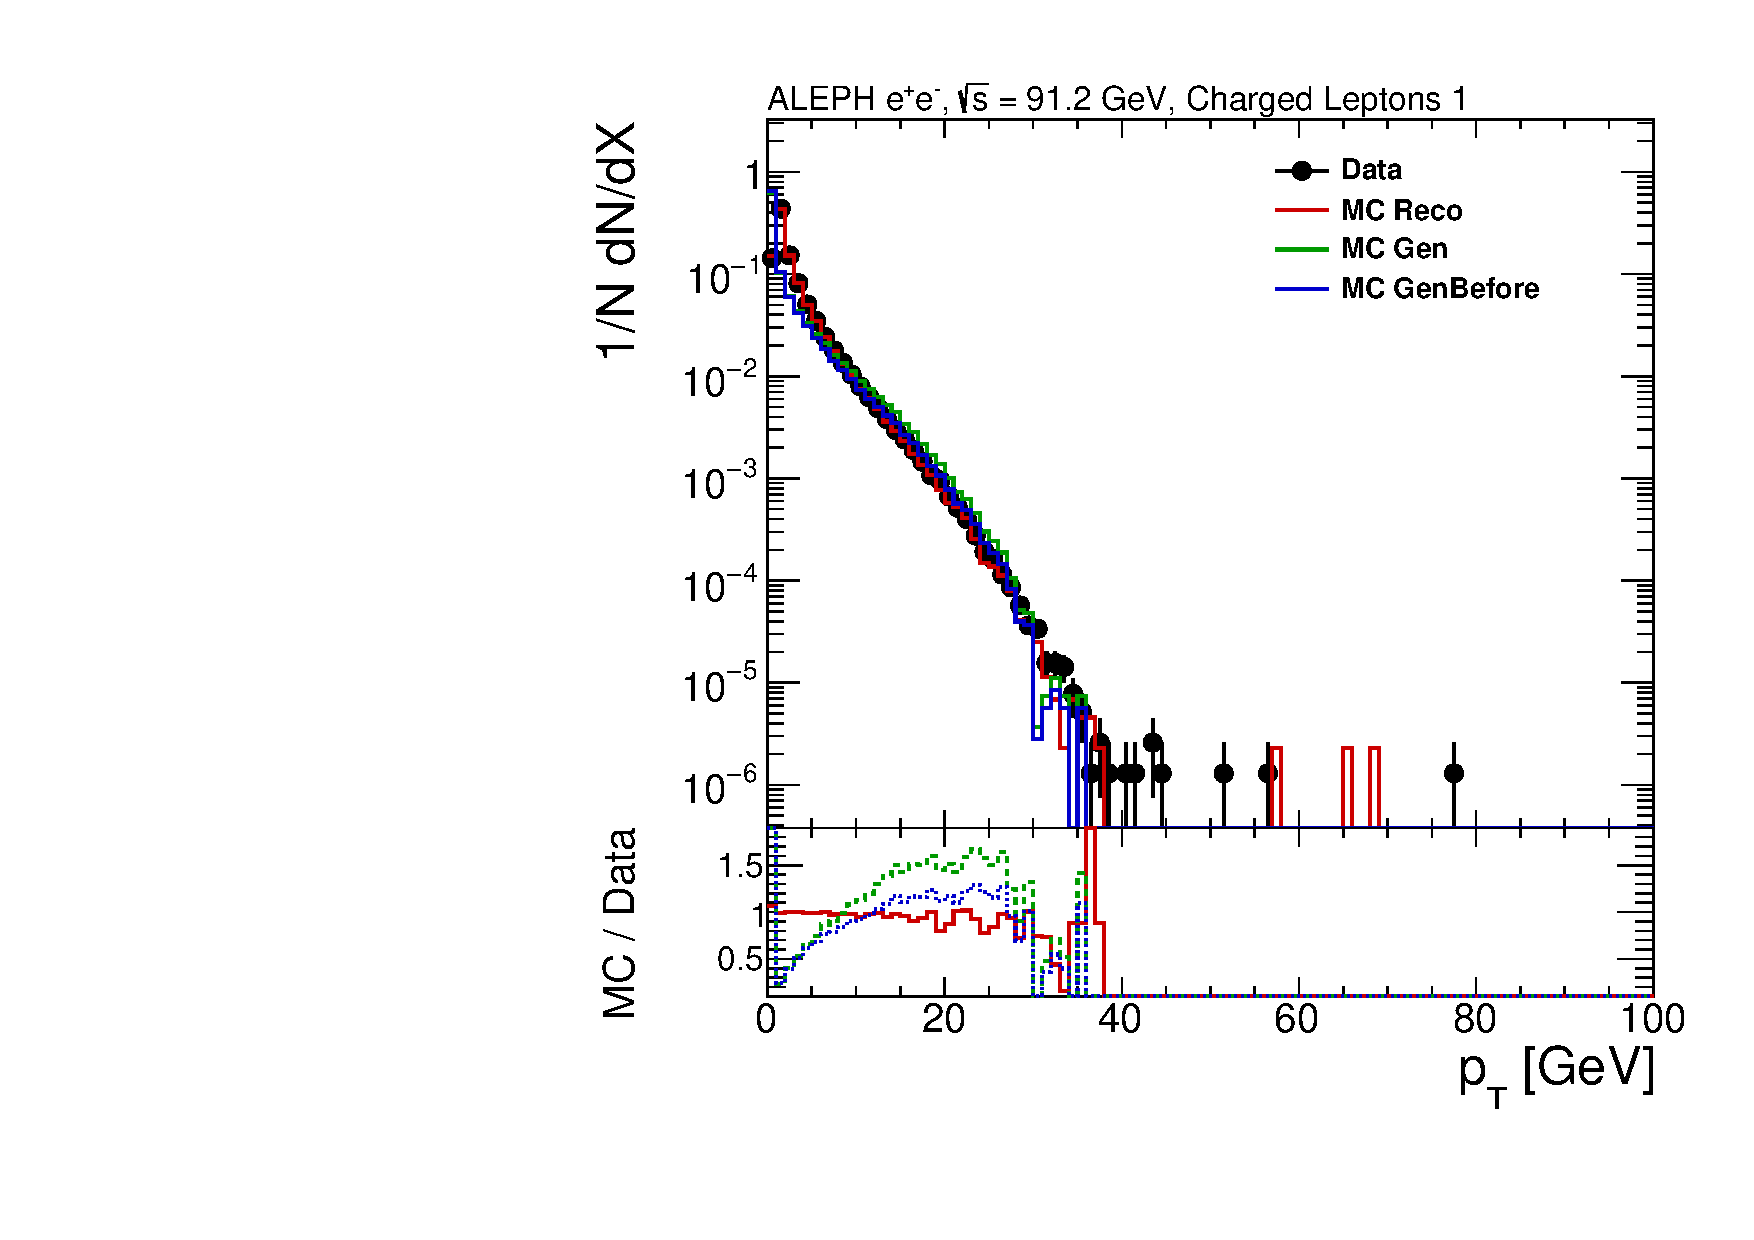
\includegraphics[width=0.325\textwidth]{../Studies/PreliminaryResult/2026-02-17_thrust_iter5/pwflag_kinematics/pwflag1_pt.pdf}
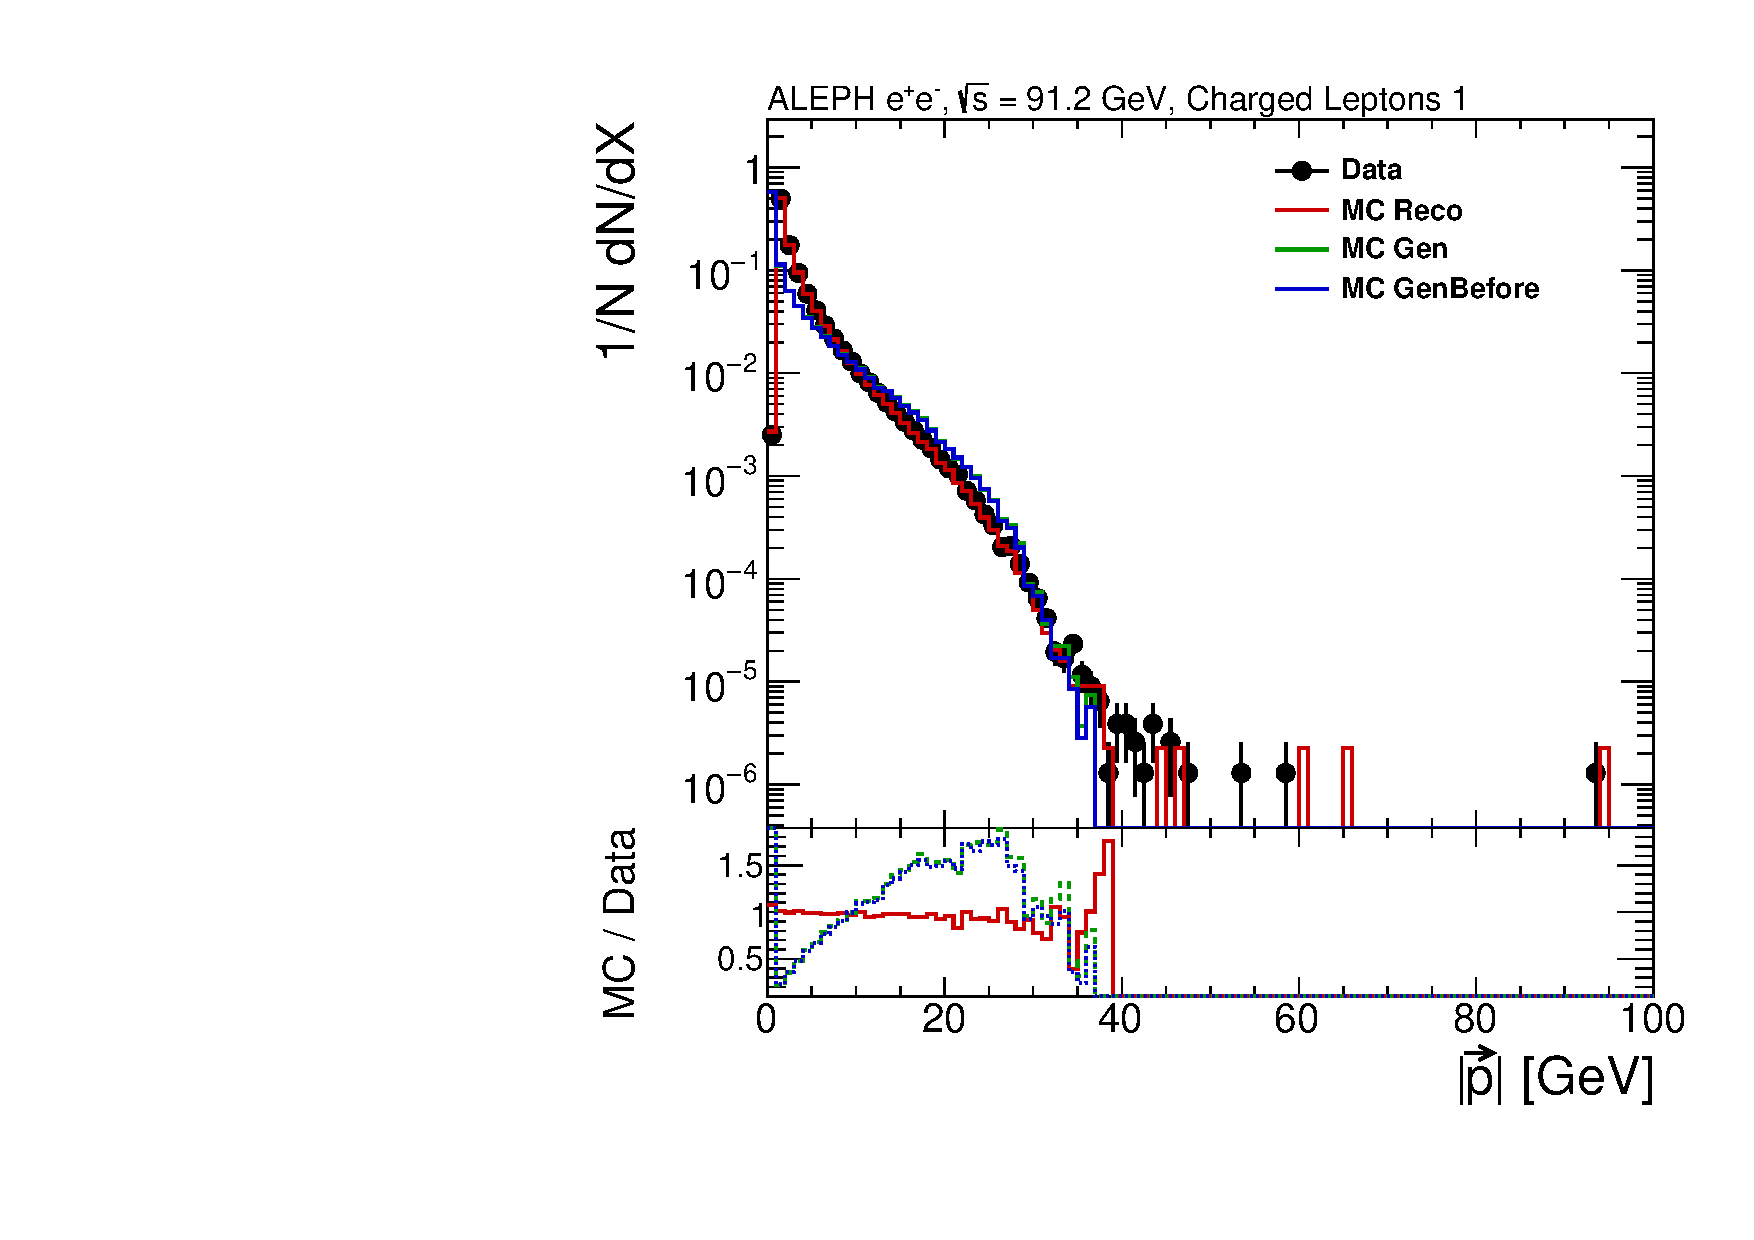
\includegraphics[width=0.325\textwidth]{../Studies/PreliminaryResult/2026-02-17_thrust_iter5/pwflag_kinematics/pwflag1_pmag.pdf}
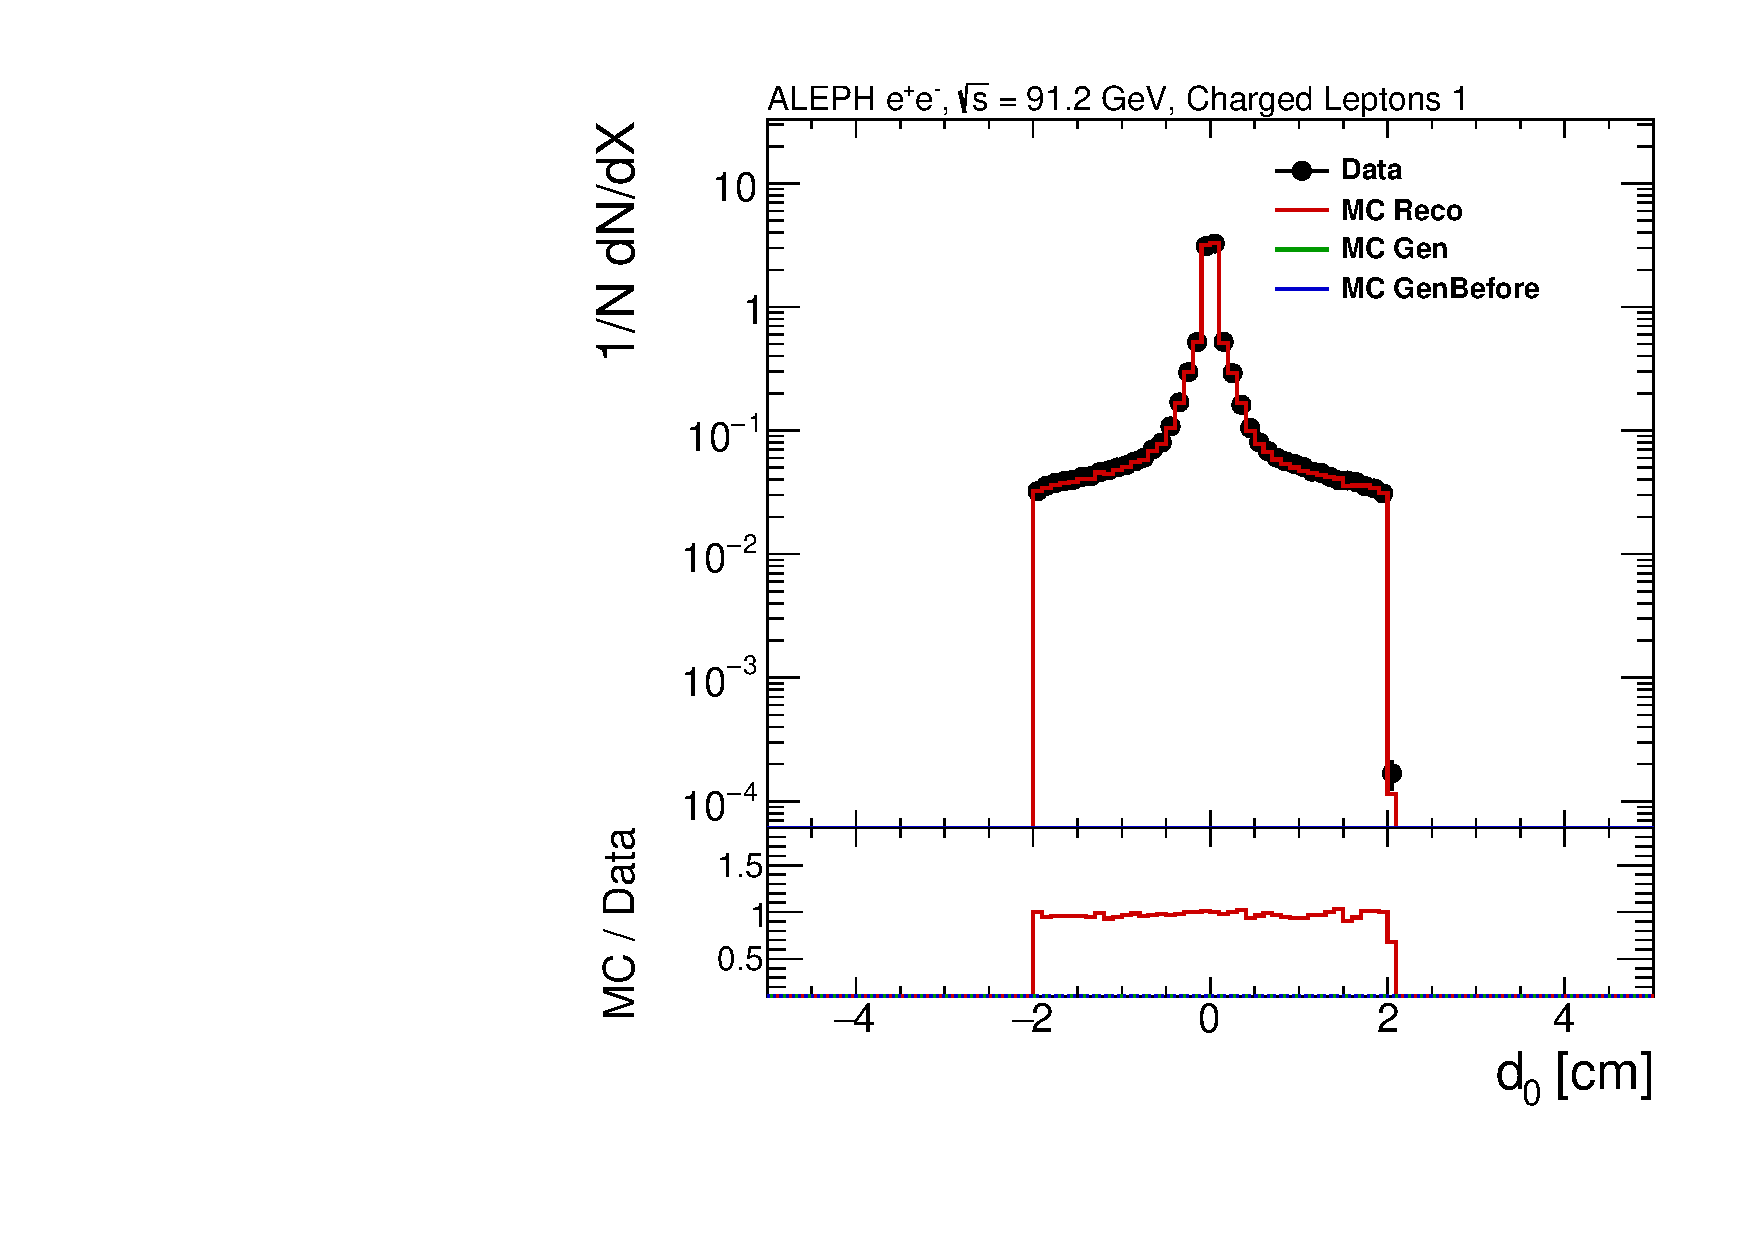
\includegraphics[width=0.325\textwidth]{../Studies/PreliminaryResult/2026-02-17_thrust_iter5/pwflag_kinematics/pwflag1_d0.pdf}
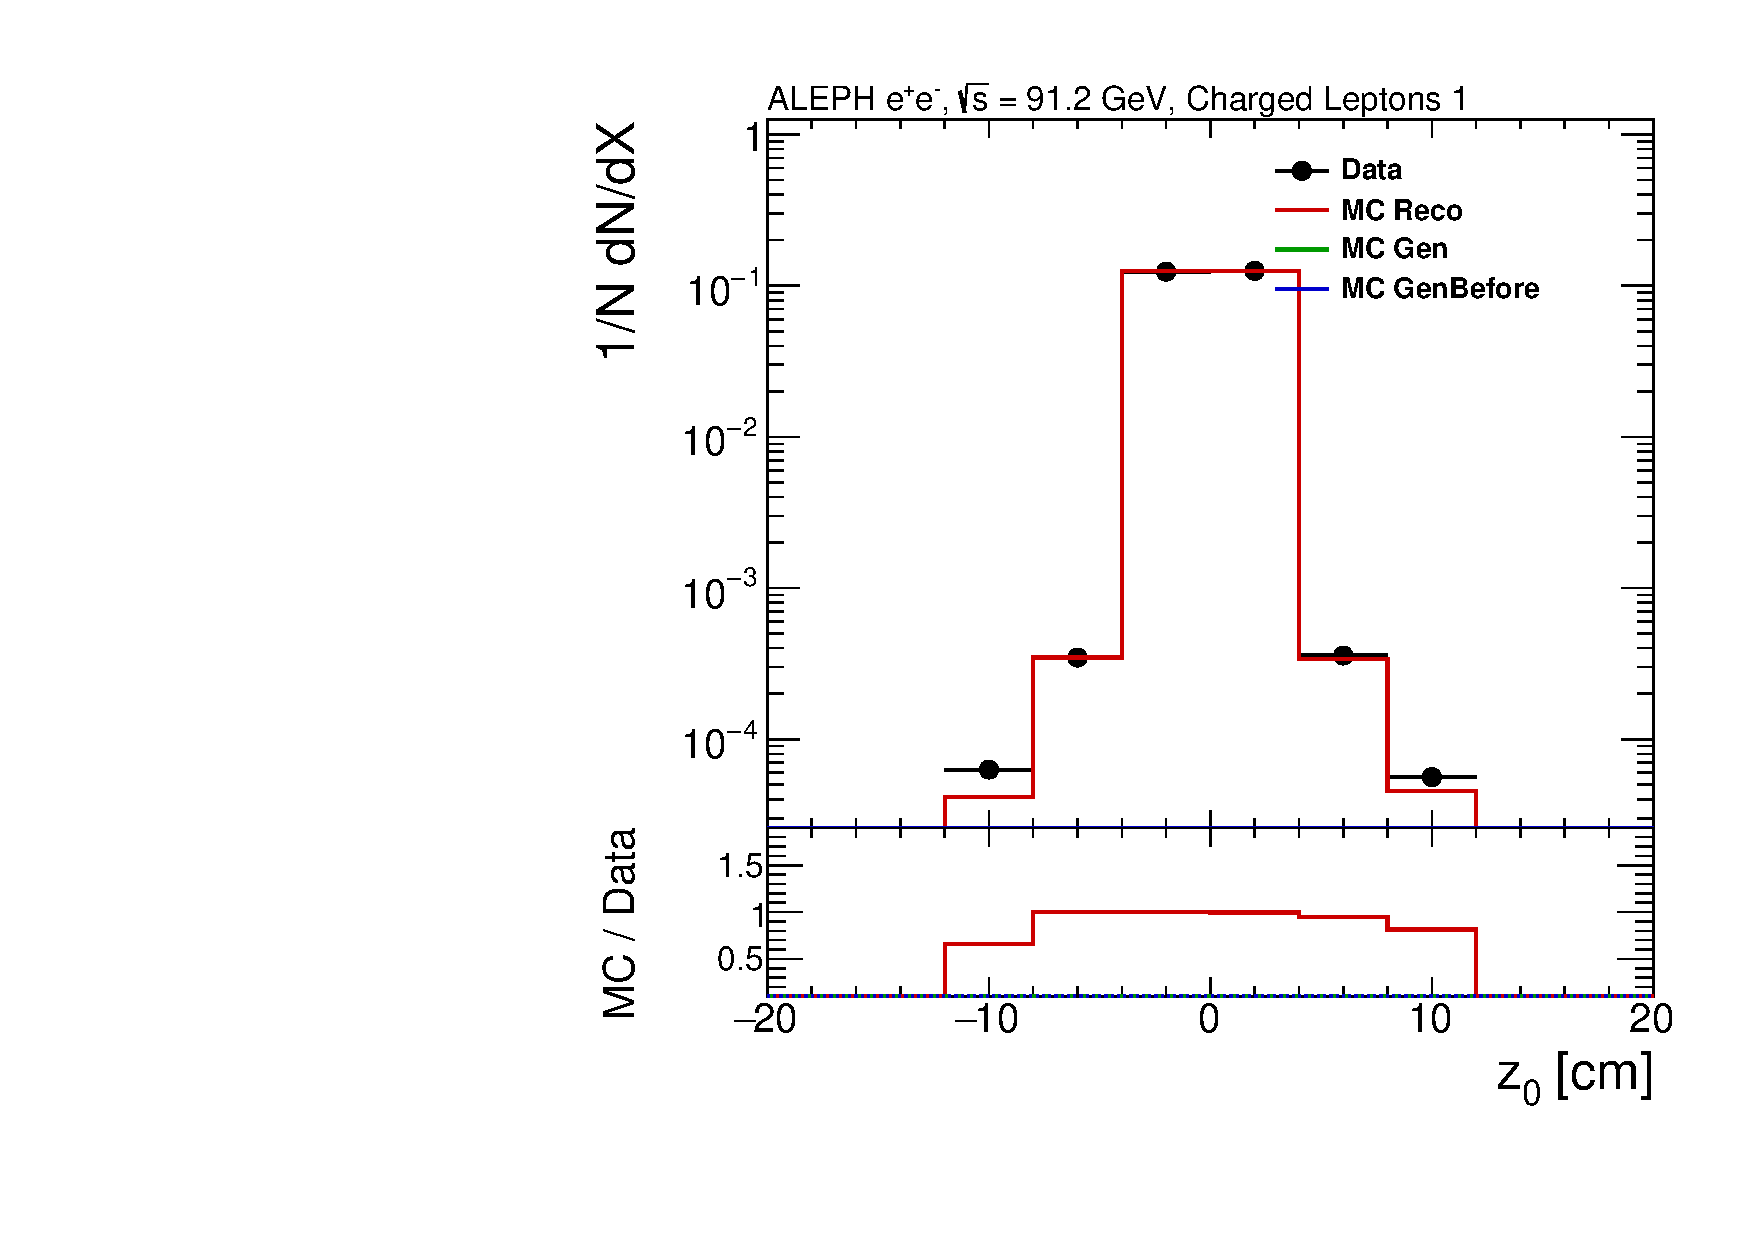
\includegraphics[width=0.325\textwidth]{../Studies/PreliminaryResult/2026-02-17_thrust_iter5/pwflag_kinematics/pwflag1_z0.pdf}
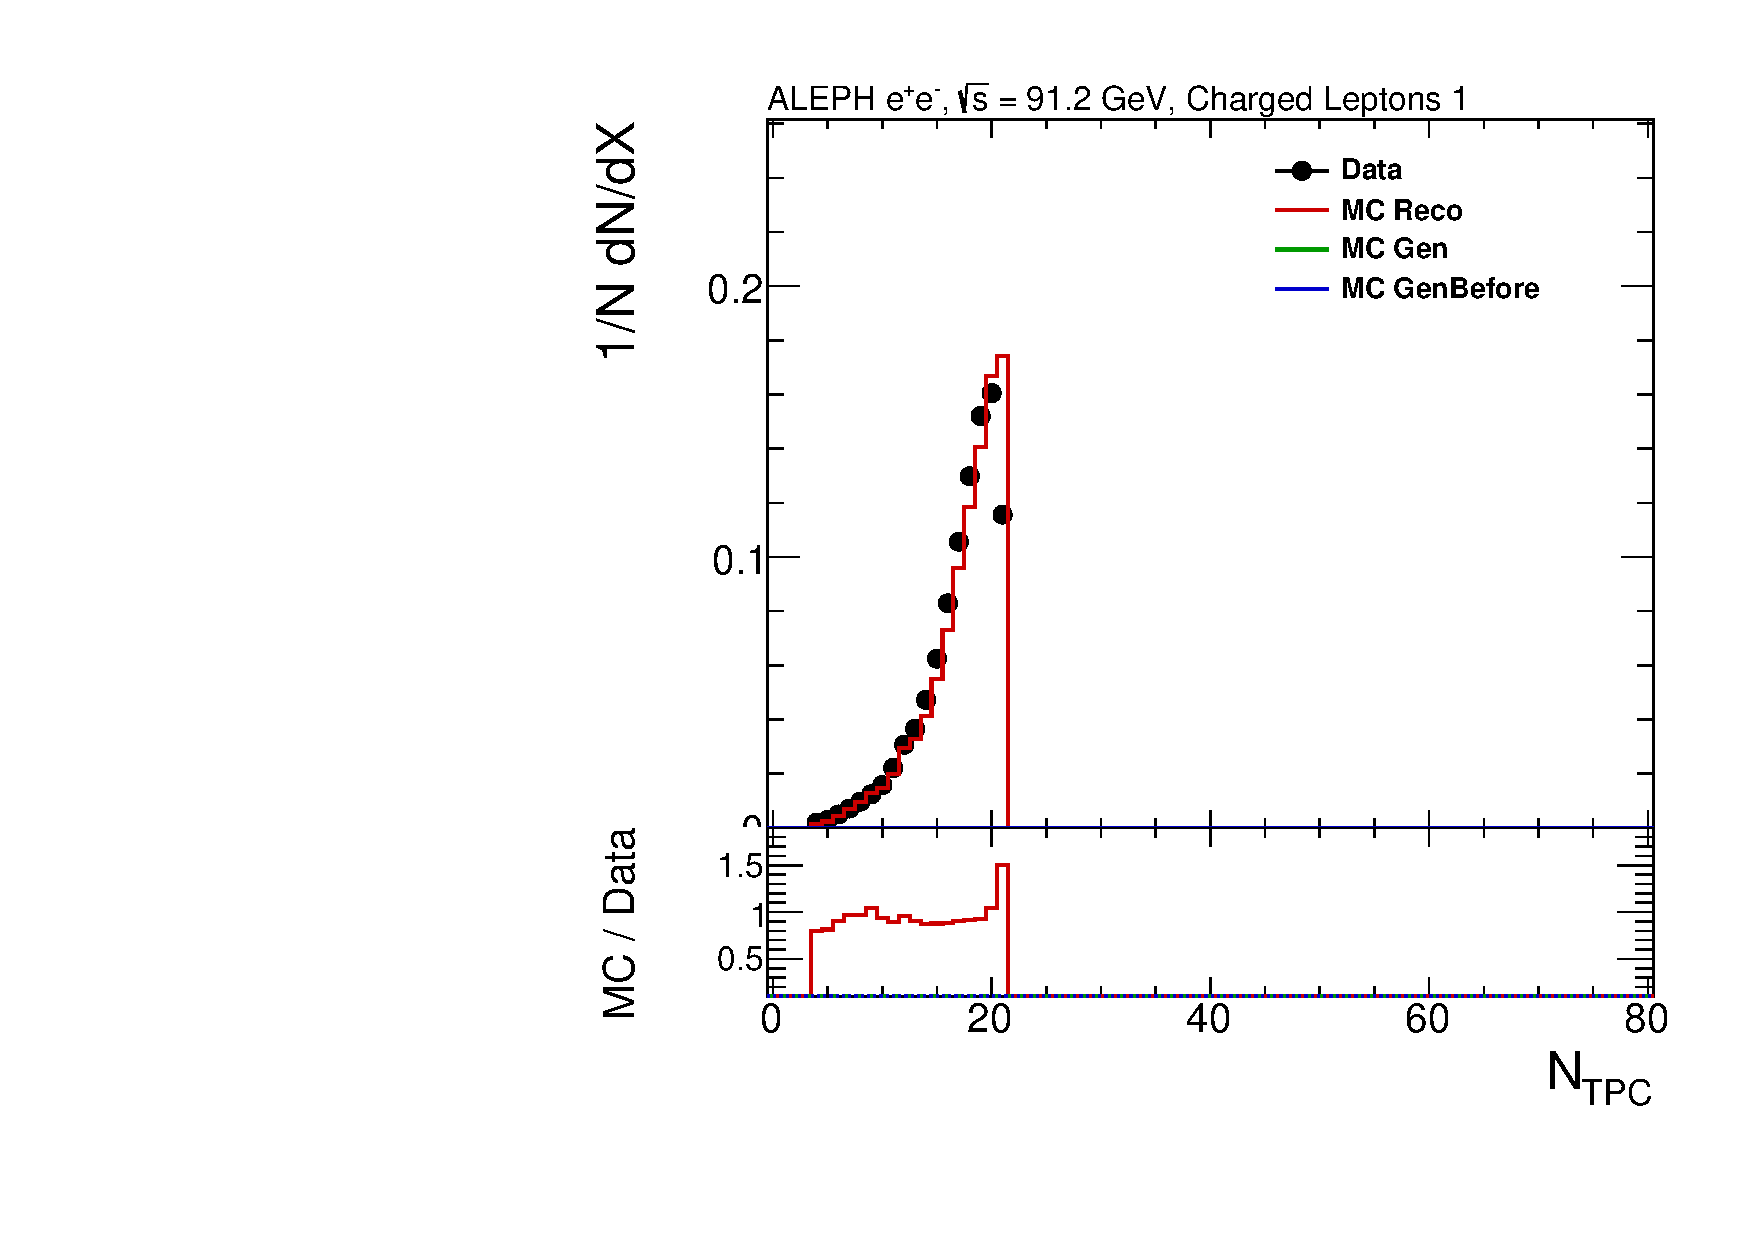
\includegraphics[width=0.325\textwidth]{../Studies/PreliminaryResult/2026-02-17_thrust_iter5/pwflag_kinematics/pwflag1_ntpc.pdf}
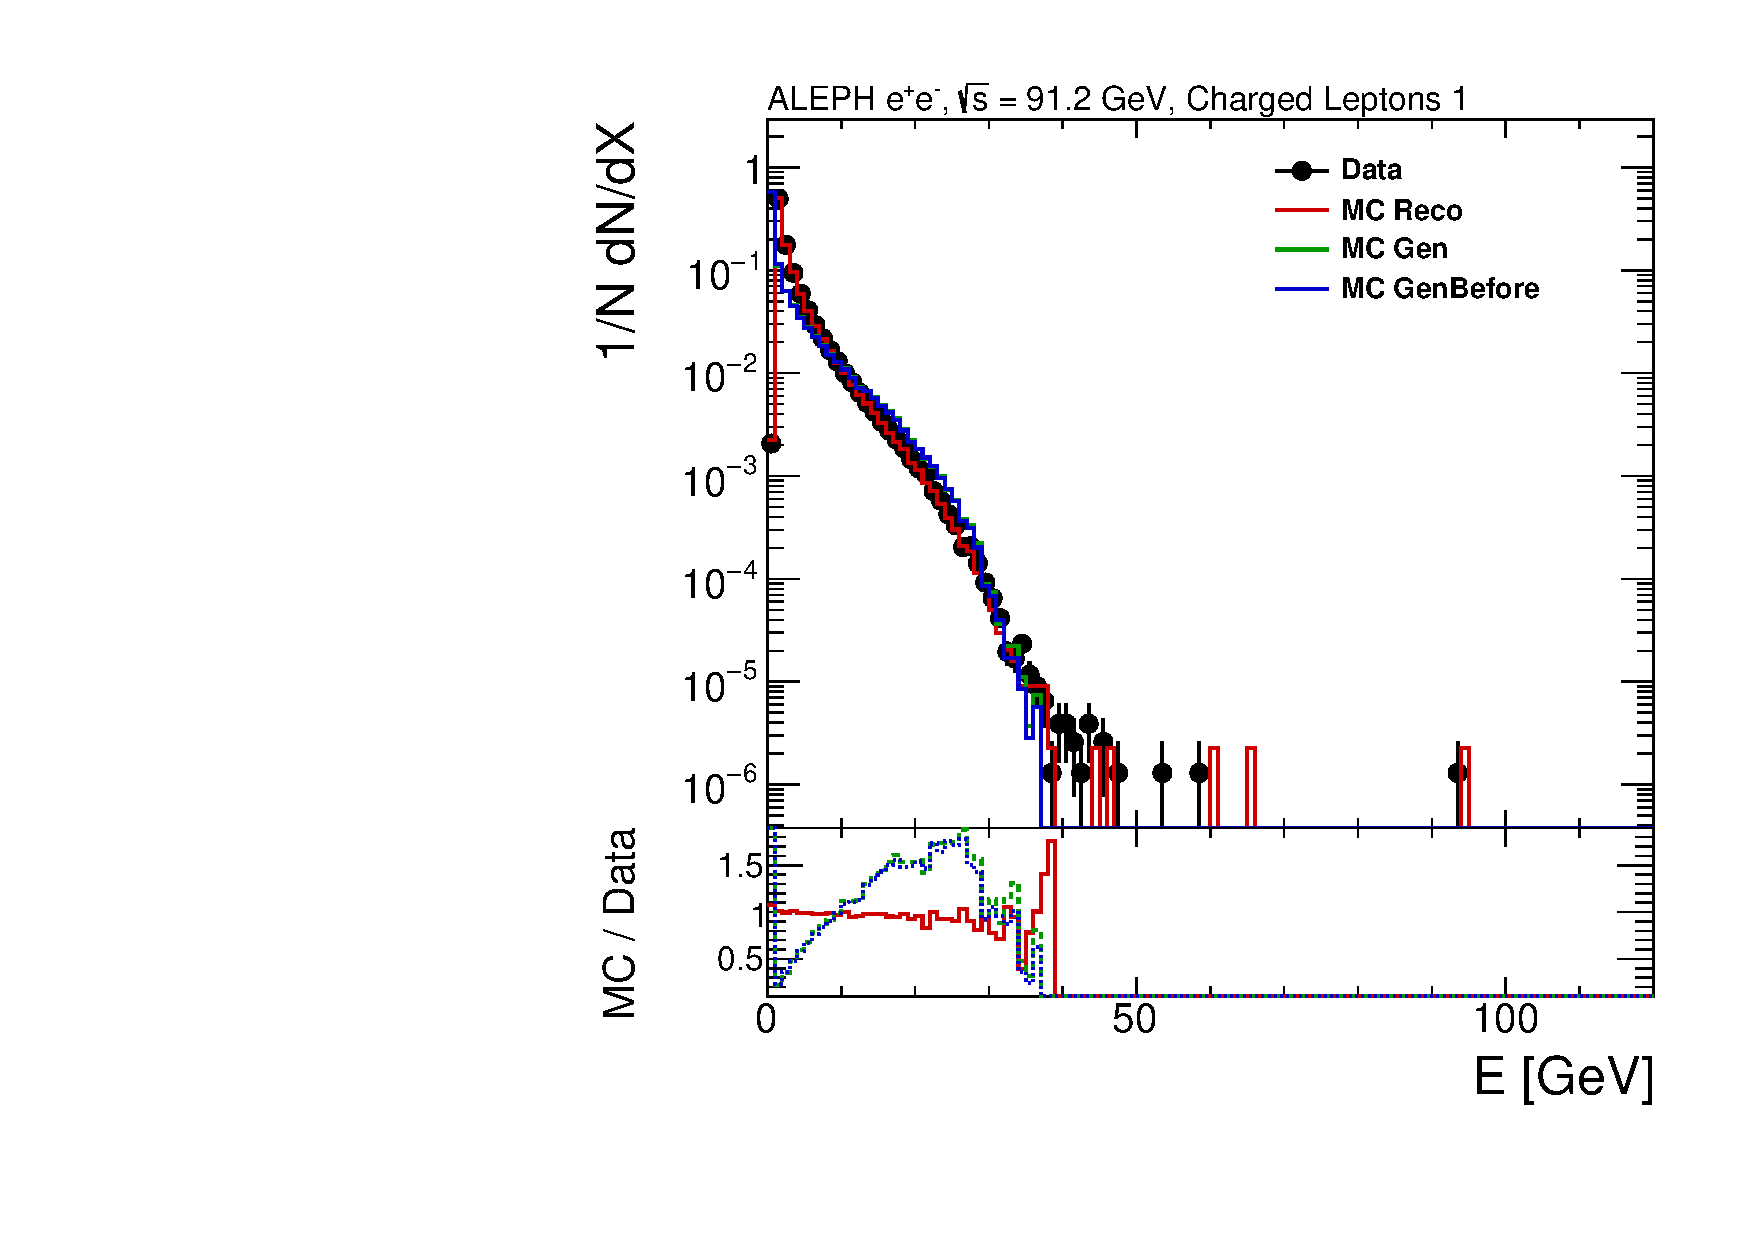
\includegraphics[width=0.325\textwidth]{../Studies/PreliminaryResult/2026-02-17_thrust_iter5/pwflag_kinematics/pwflag1_energy.pdf}
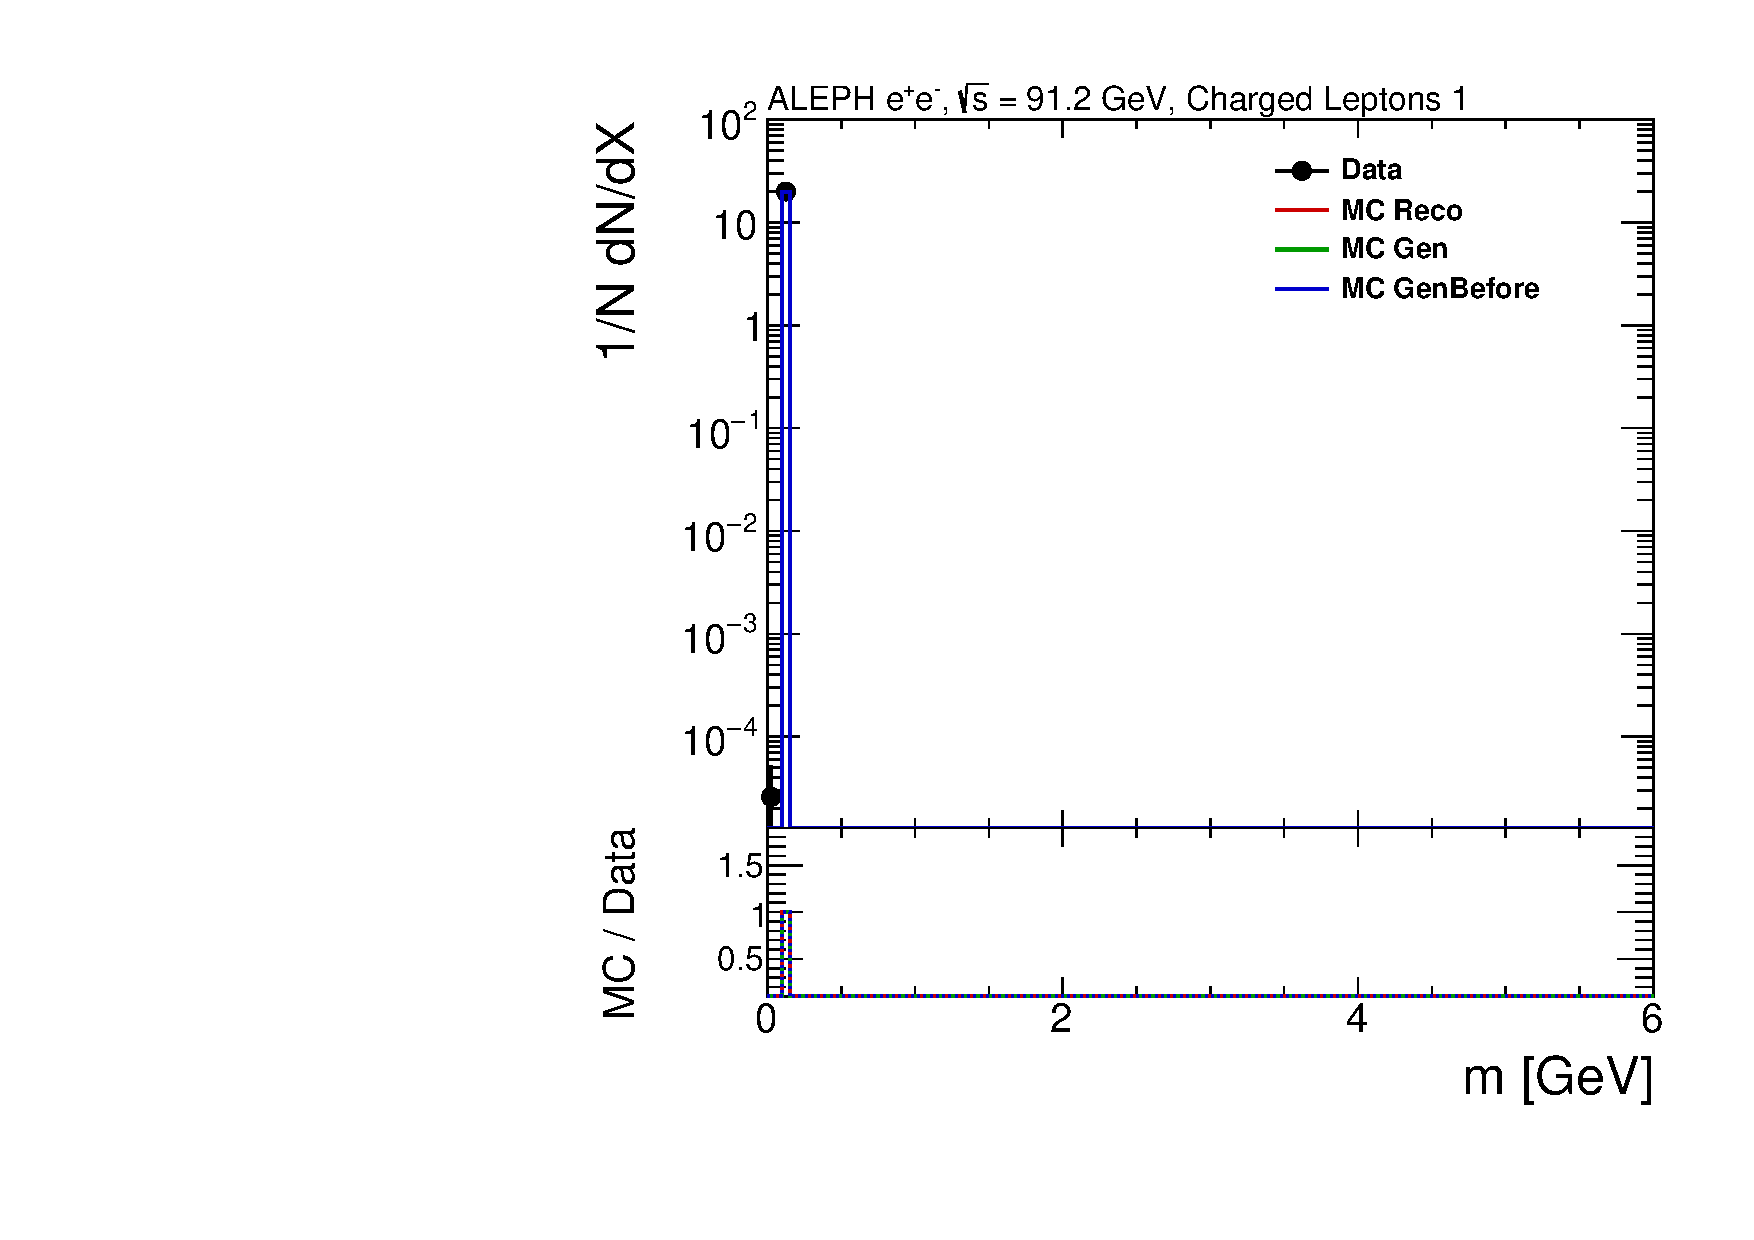
\includegraphics[width=0.325\textwidth]{../Studies/PreliminaryResult/2026-02-17_thrust_iter5/pwflag_kinematics/pwflag1_mass.pdf}
\caption{Complete \texttt{pwflag}=1 kinematic set.}
\label{fig:pwflag1_full}
\end{figure}

\noindent
Figure~\ref{fig:pwflag1_full} shows the first charged-lepton class used in the nominal object
list; these lower-rate objects still affect event axes in asymmetric topologies. Relative to
charged tracks, this category has smaller yields and larger statistical fluctuations, but the
detector-level and MC shapes remain consistent across the main selection observables. The
comparison is important because isolated energetic leptons can rotate the thrust axis in otherwise
two-jet-like events and can therefore influence migration in specific bins.

\begin{figure}[t!]
\centering
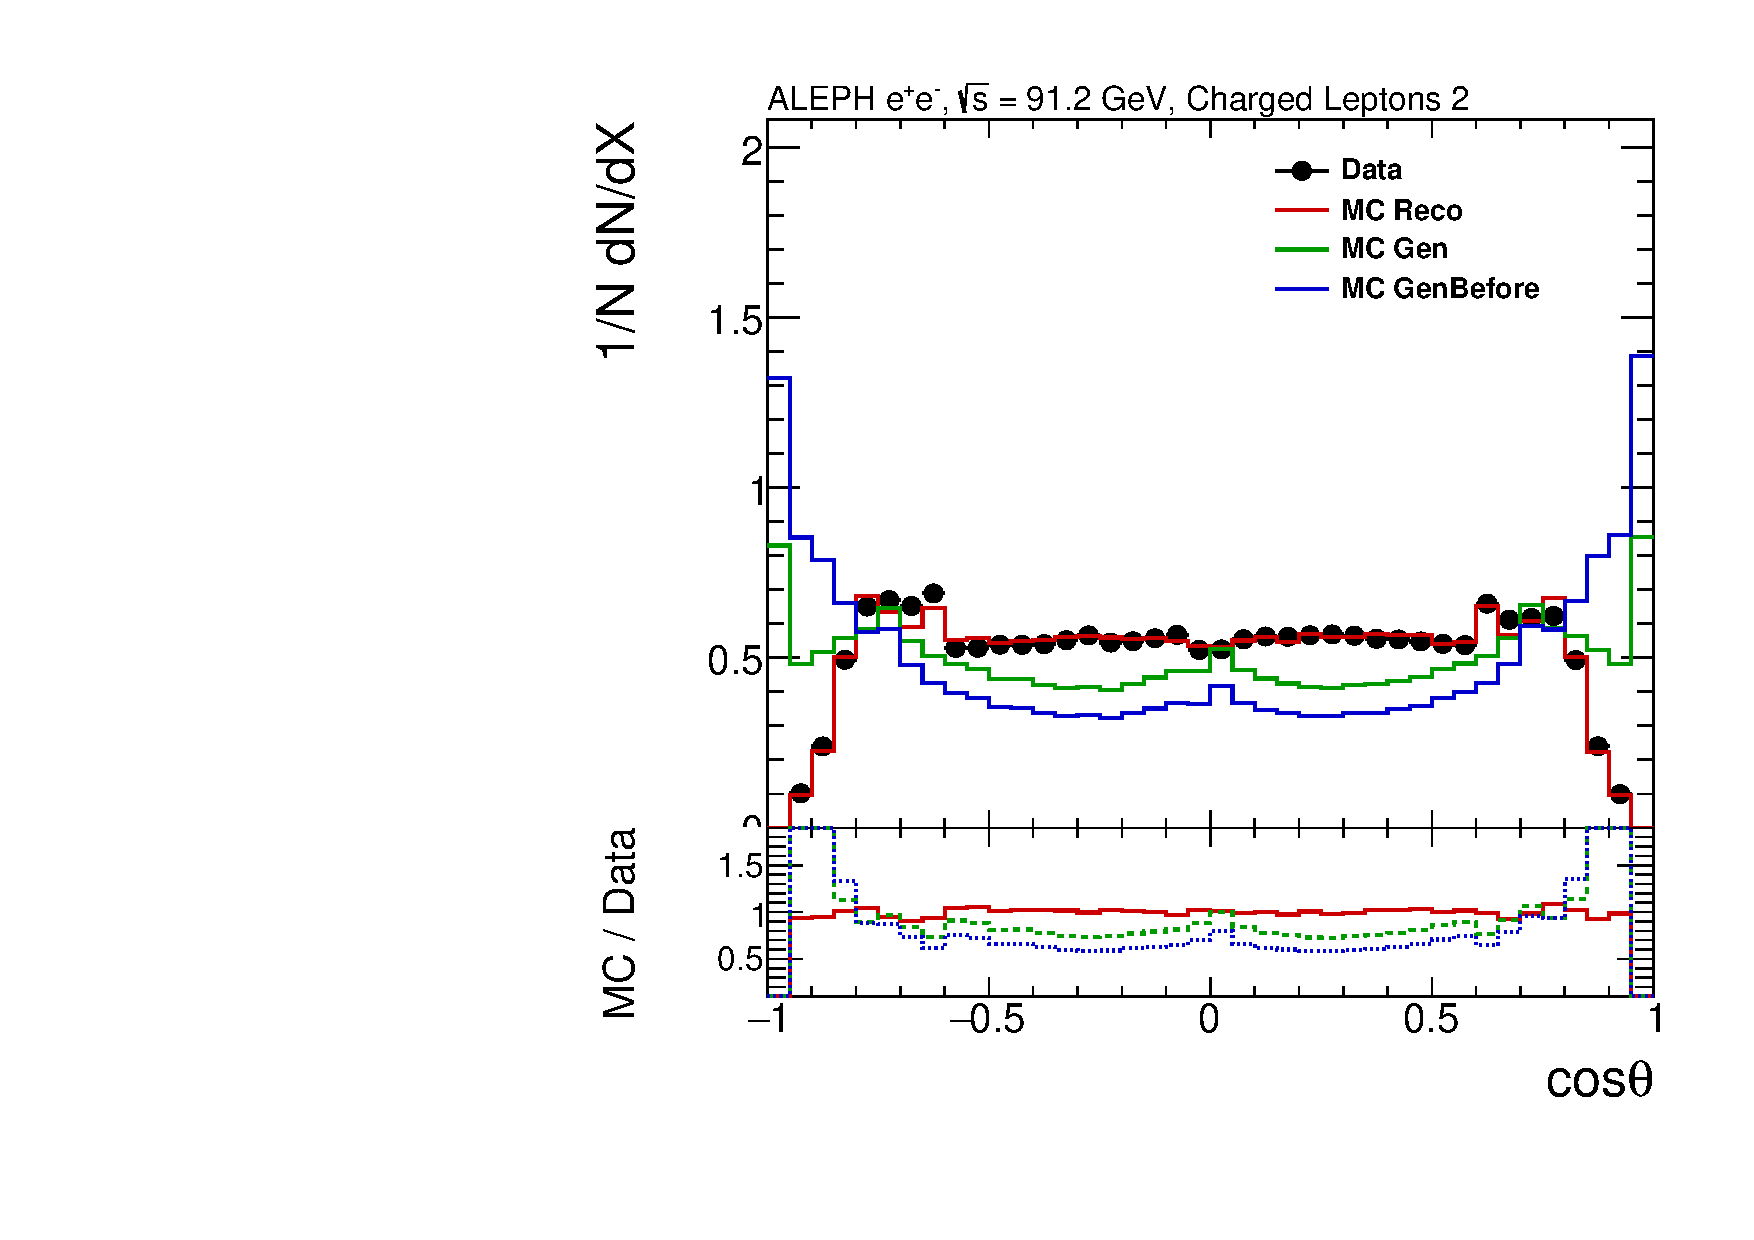
\includegraphics[width=0.325\textwidth]{../Studies/PreliminaryResult/2026-02-17_thrust_iter5/pwflag_kinematics/pwflag2_cosTheta.pdf}
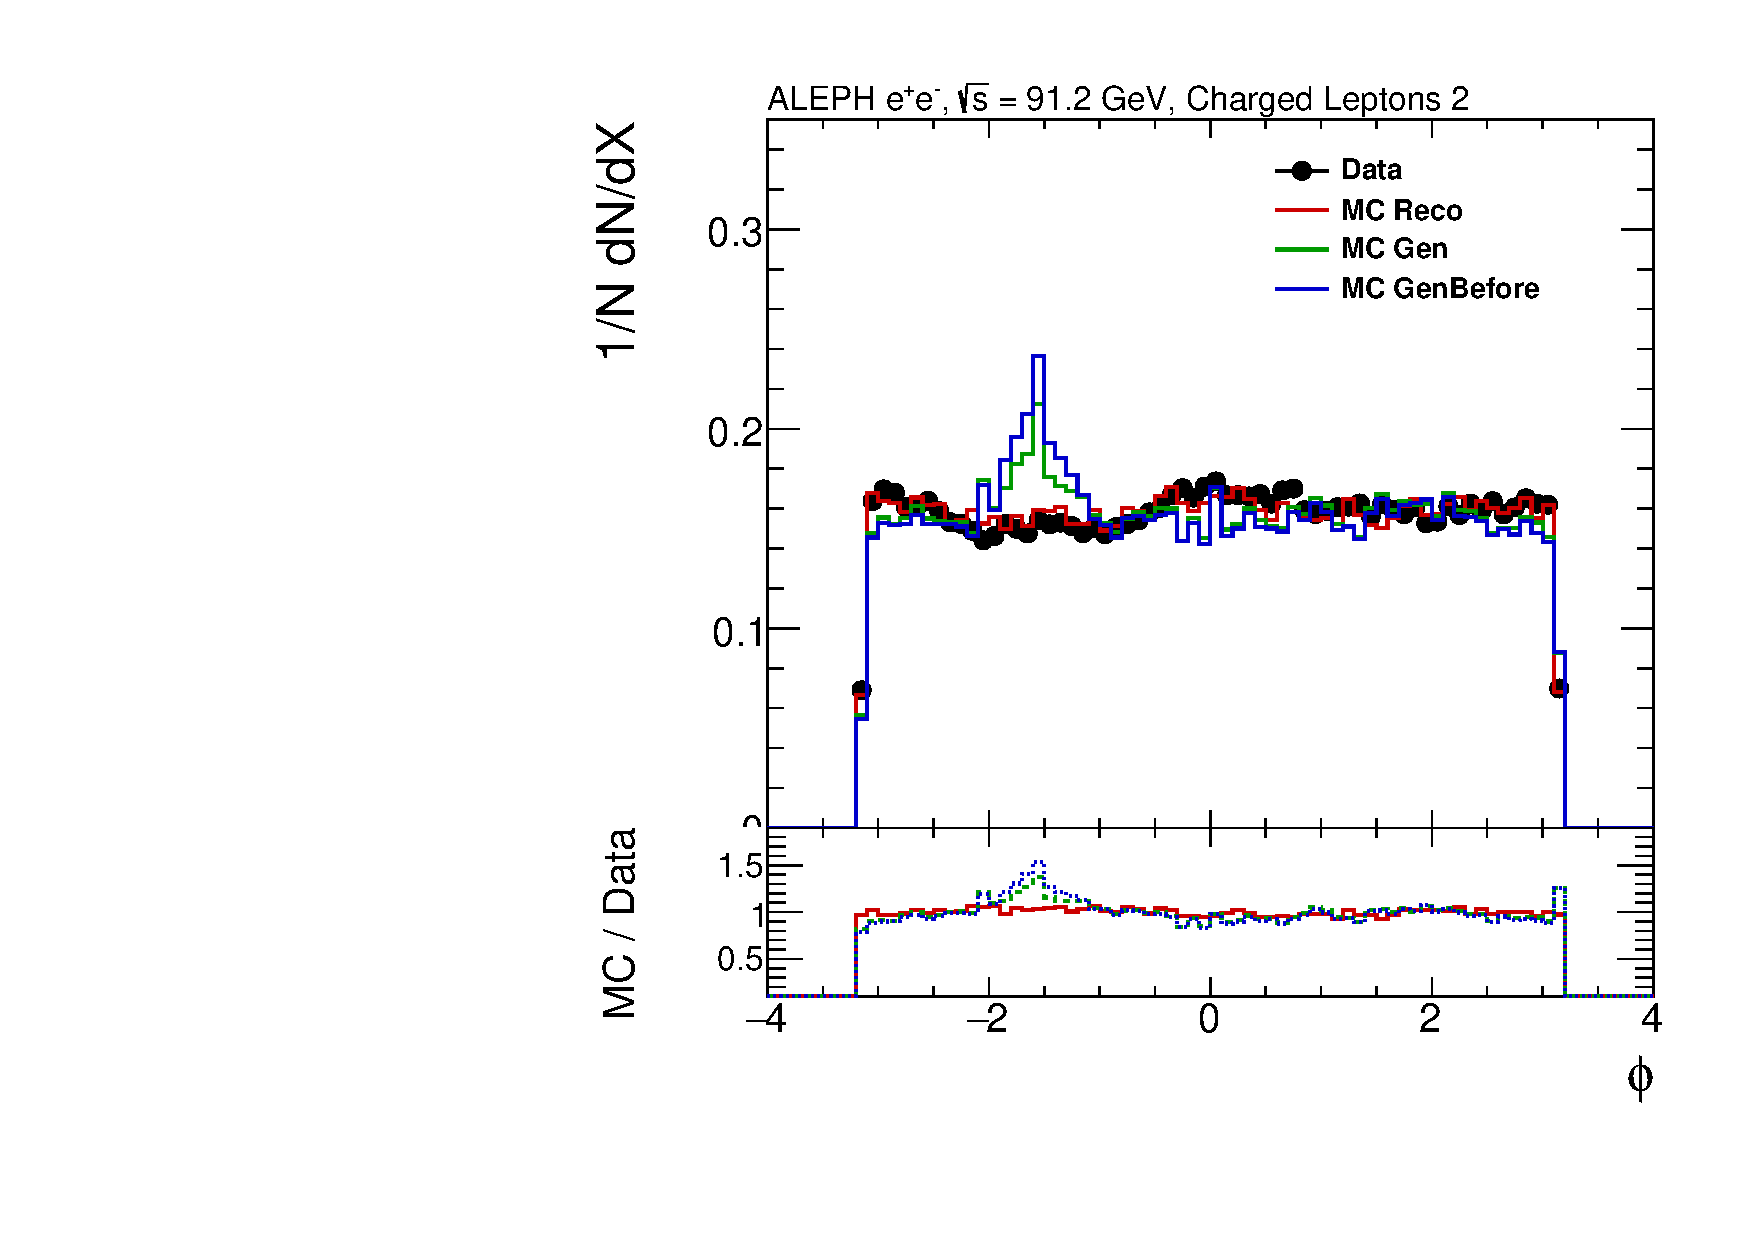
\includegraphics[width=0.325\textwidth]{../Studies/PreliminaryResult/2026-02-17_thrust_iter5/pwflag_kinematics/pwflag2_phi.pdf}
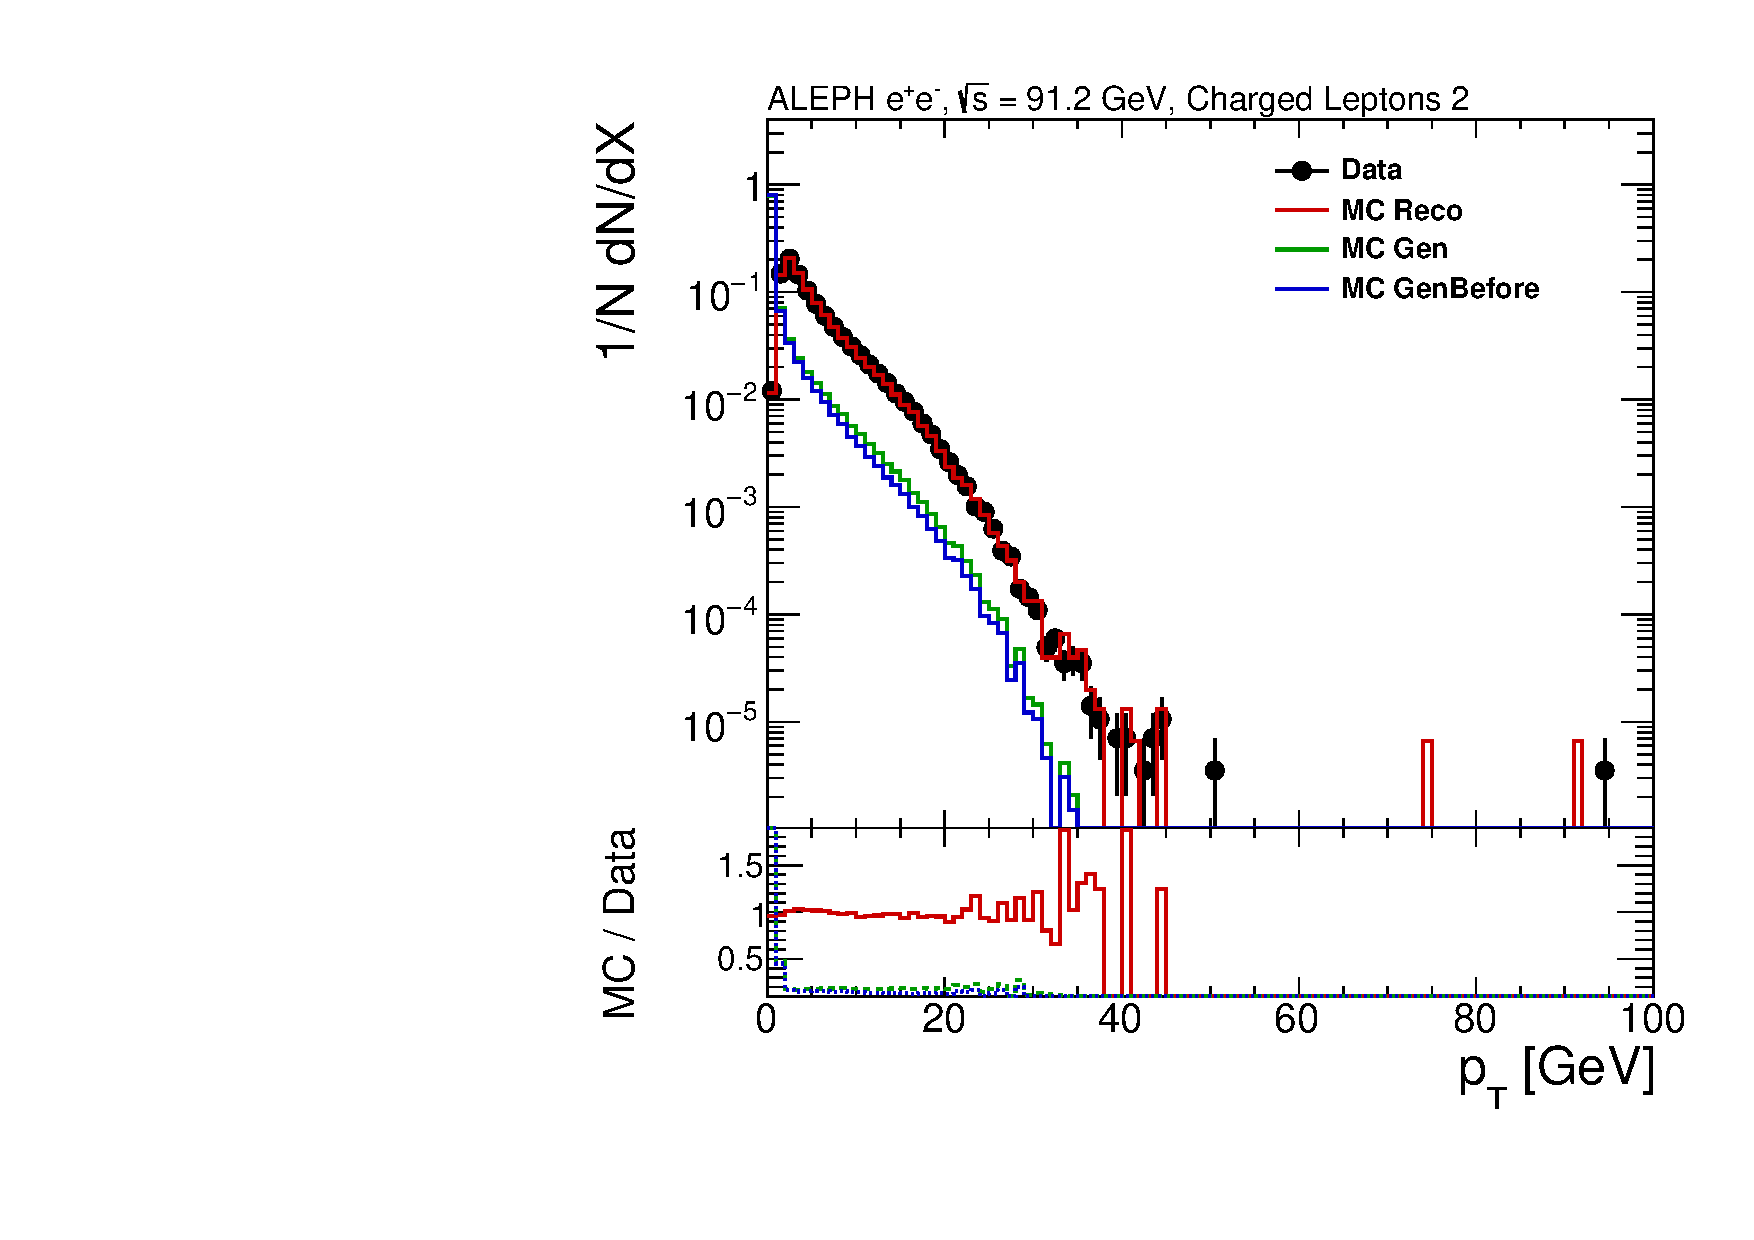
\includegraphics[width=0.325\textwidth]{../Studies/PreliminaryResult/2026-02-17_thrust_iter5/pwflag_kinematics/pwflag2_pt.pdf}
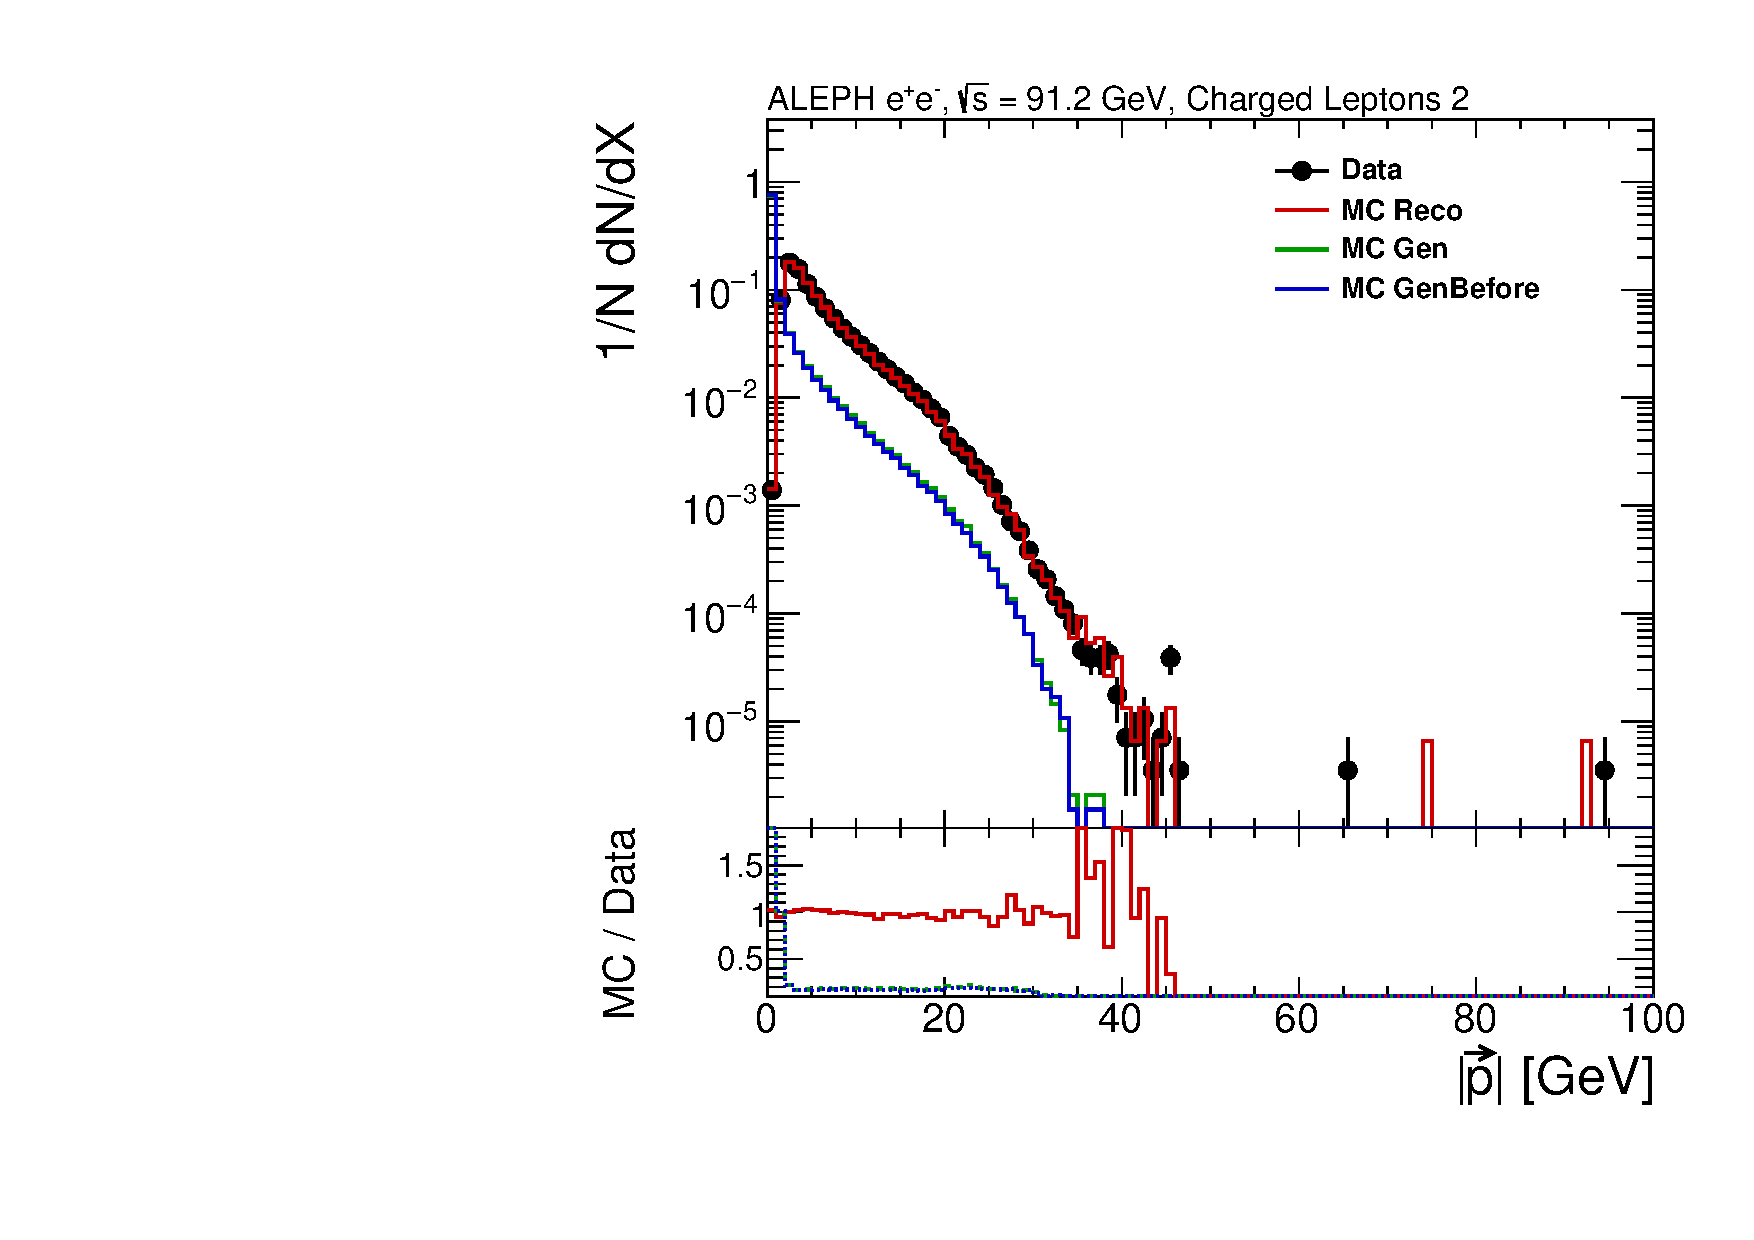
\includegraphics[width=0.325\textwidth]{../Studies/PreliminaryResult/2026-02-17_thrust_iter5/pwflag_kinematics/pwflag2_pmag.pdf}
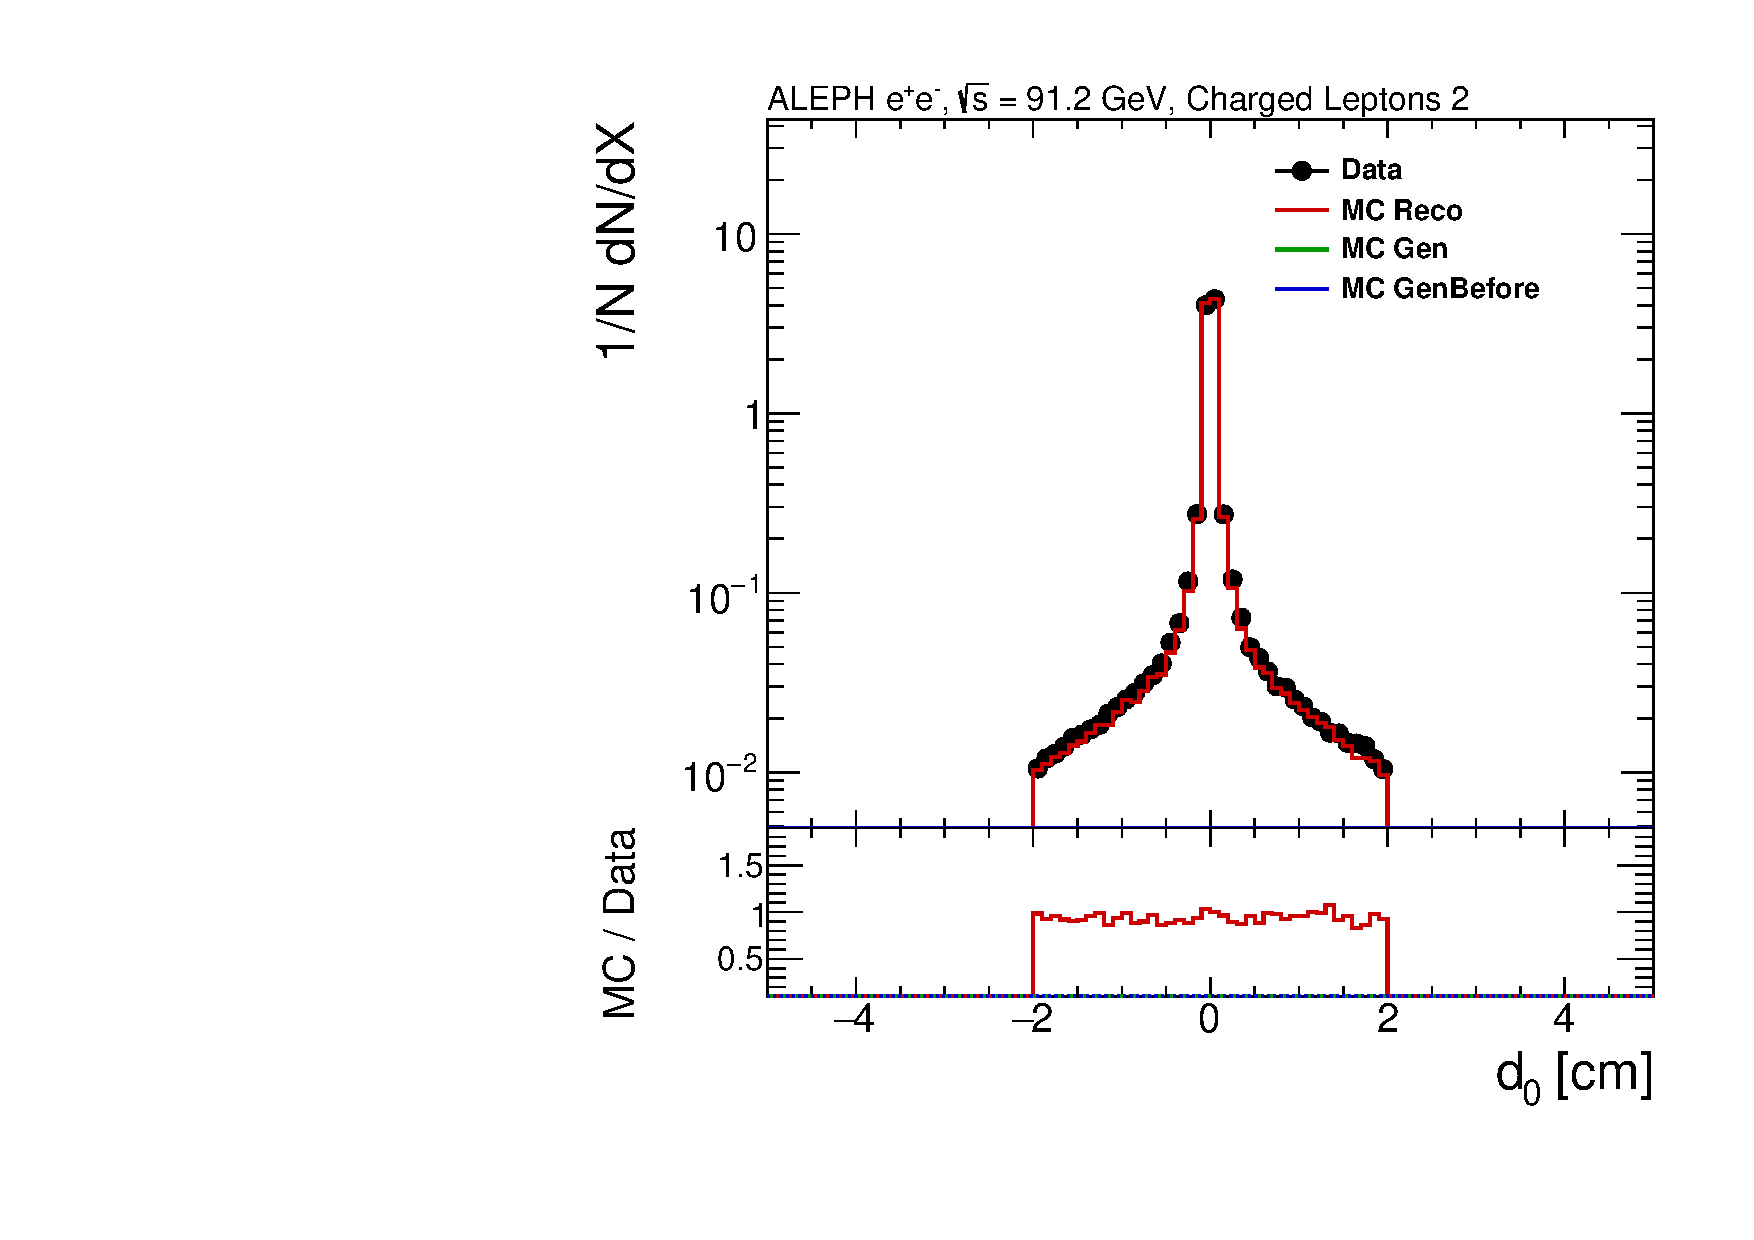
\includegraphics[width=0.325\textwidth]{../Studies/PreliminaryResult/2026-02-17_thrust_iter5/pwflag_kinematics/pwflag2_d0.pdf}
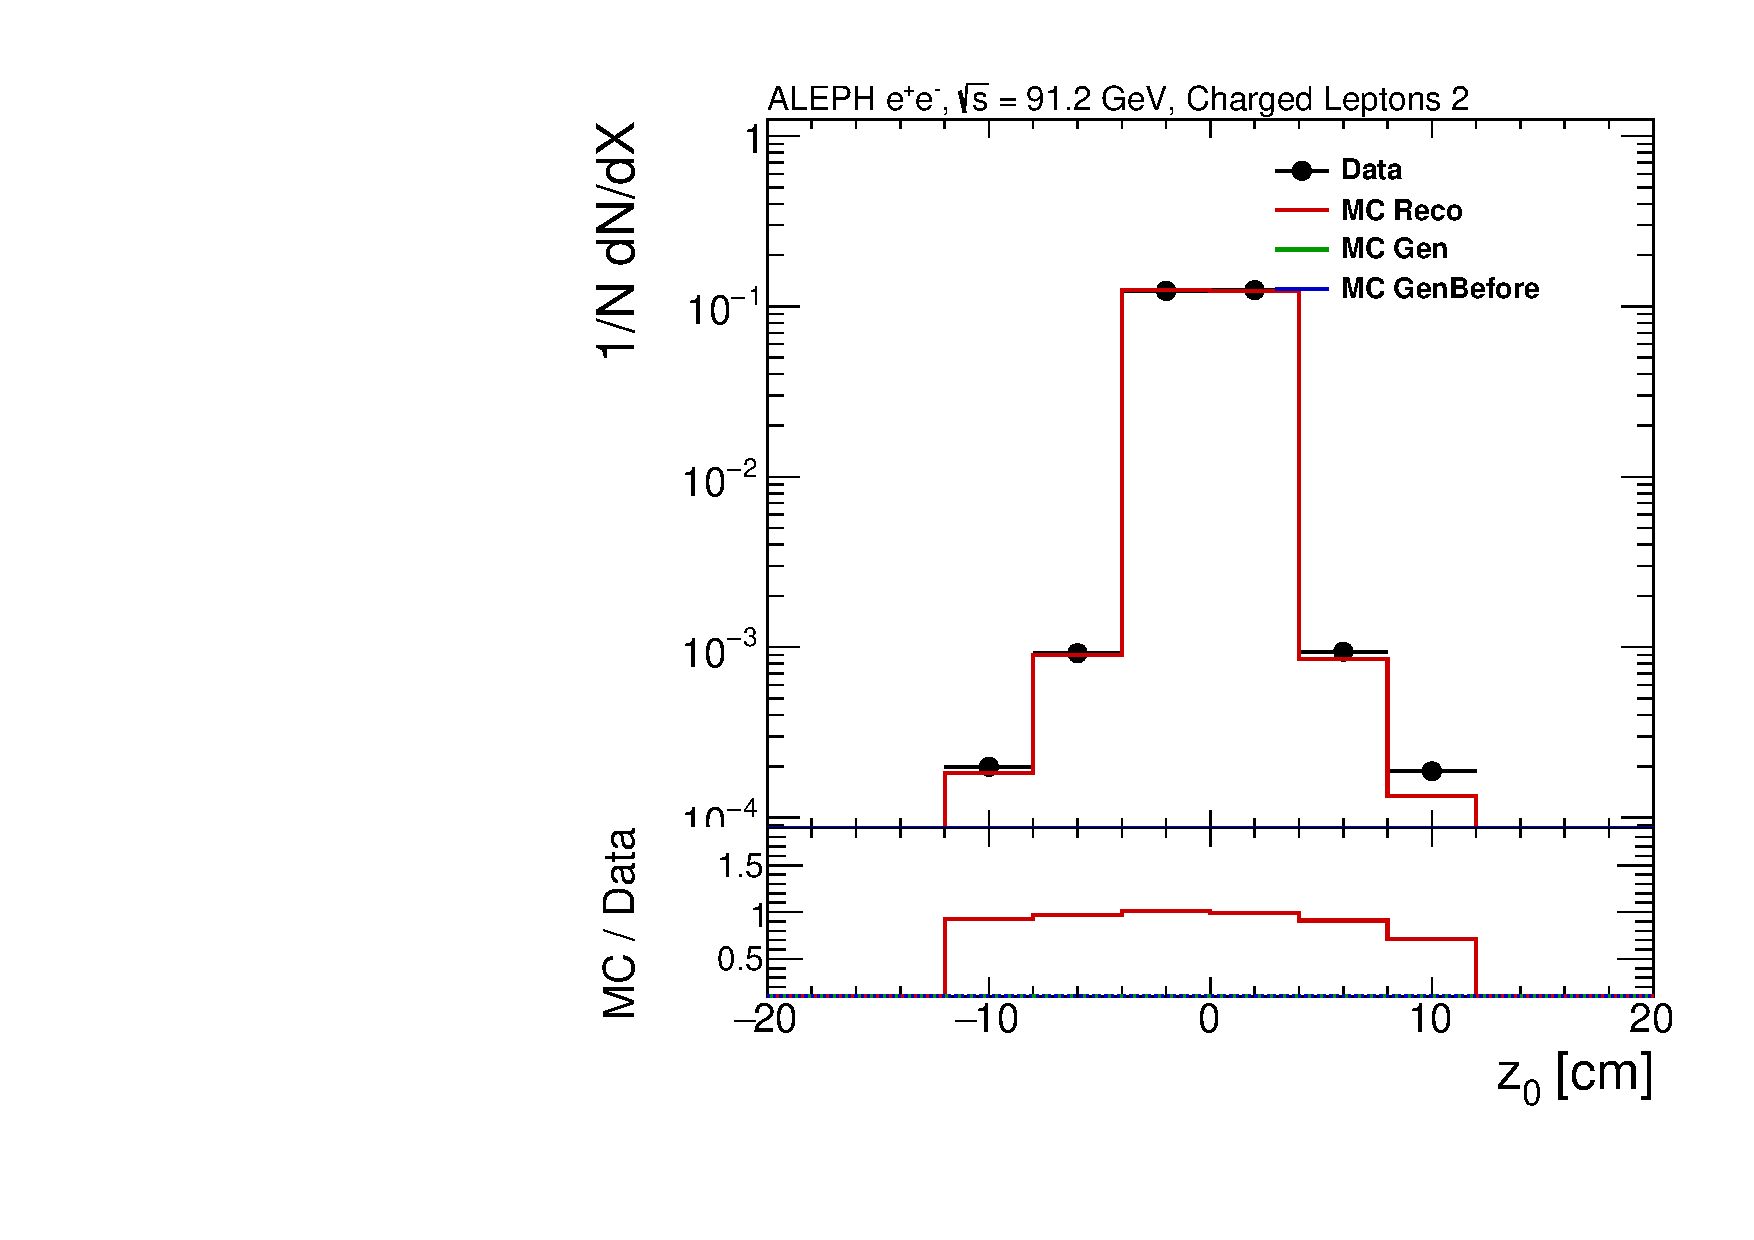
\includegraphics[width=0.325\textwidth]{../Studies/PreliminaryResult/2026-02-17_thrust_iter5/pwflag_kinematics/pwflag2_z0.pdf}
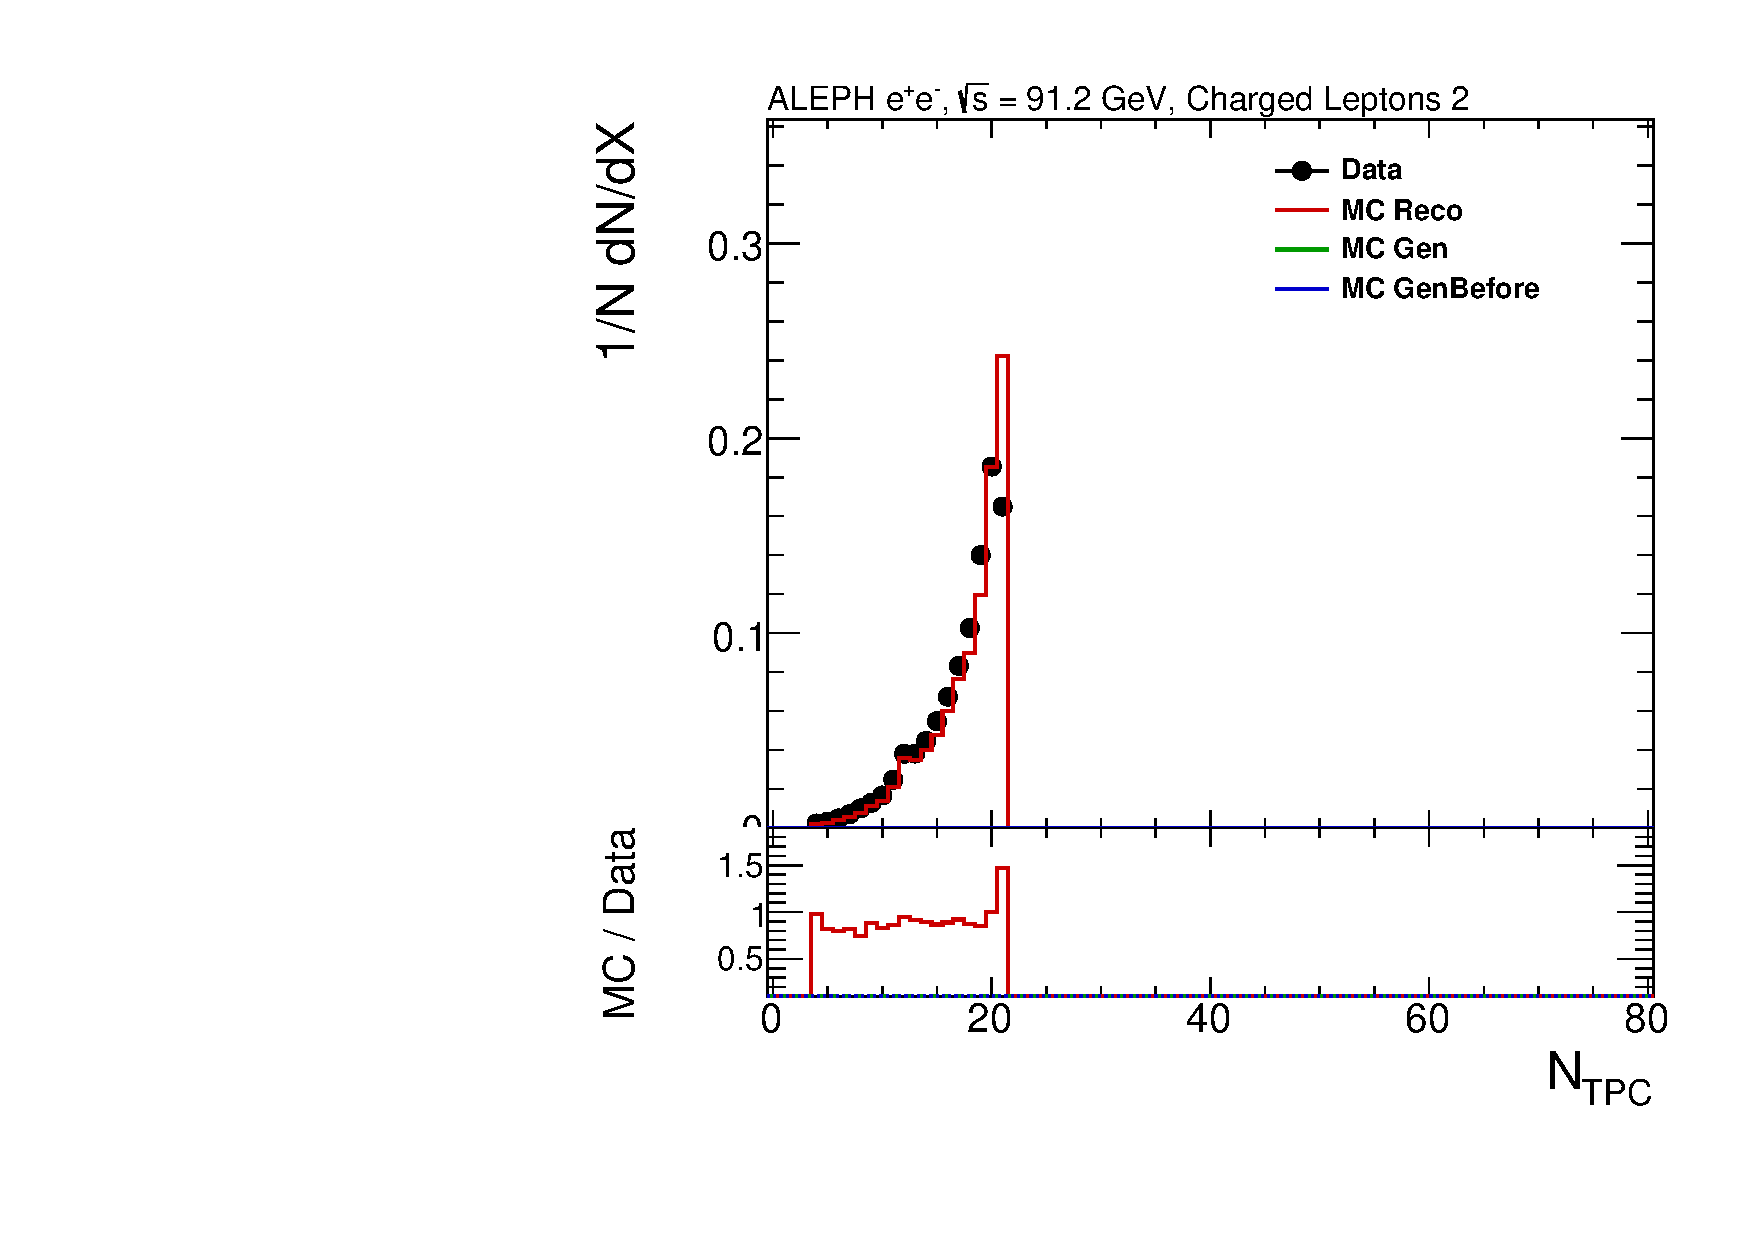
\includegraphics[width=0.325\textwidth]{../Studies/PreliminaryResult/2026-02-17_thrust_iter5/pwflag_kinematics/pwflag2_ntpc.pdf}
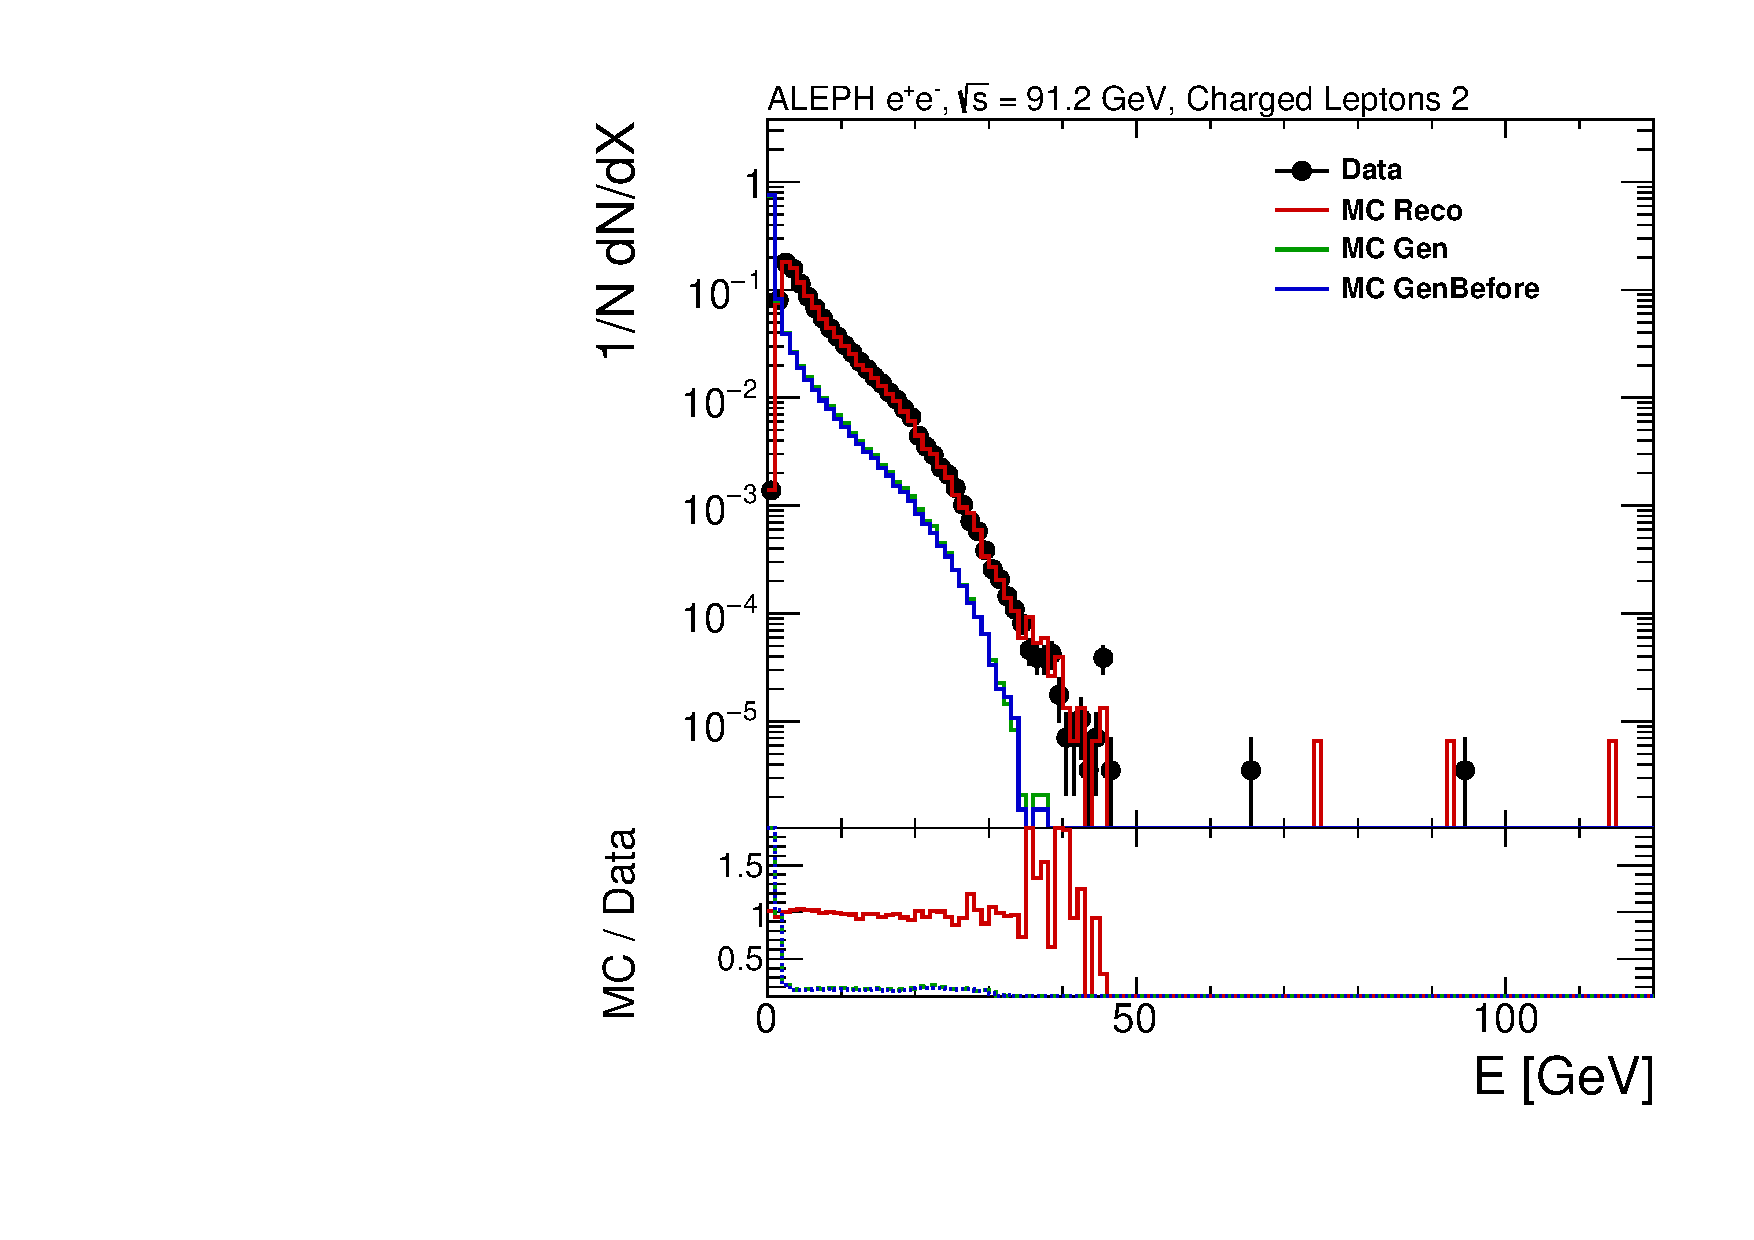
\includegraphics[width=0.325\textwidth]{../Studies/PreliminaryResult/2026-02-17_thrust_iter5/pwflag_kinematics/pwflag2_energy.pdf}
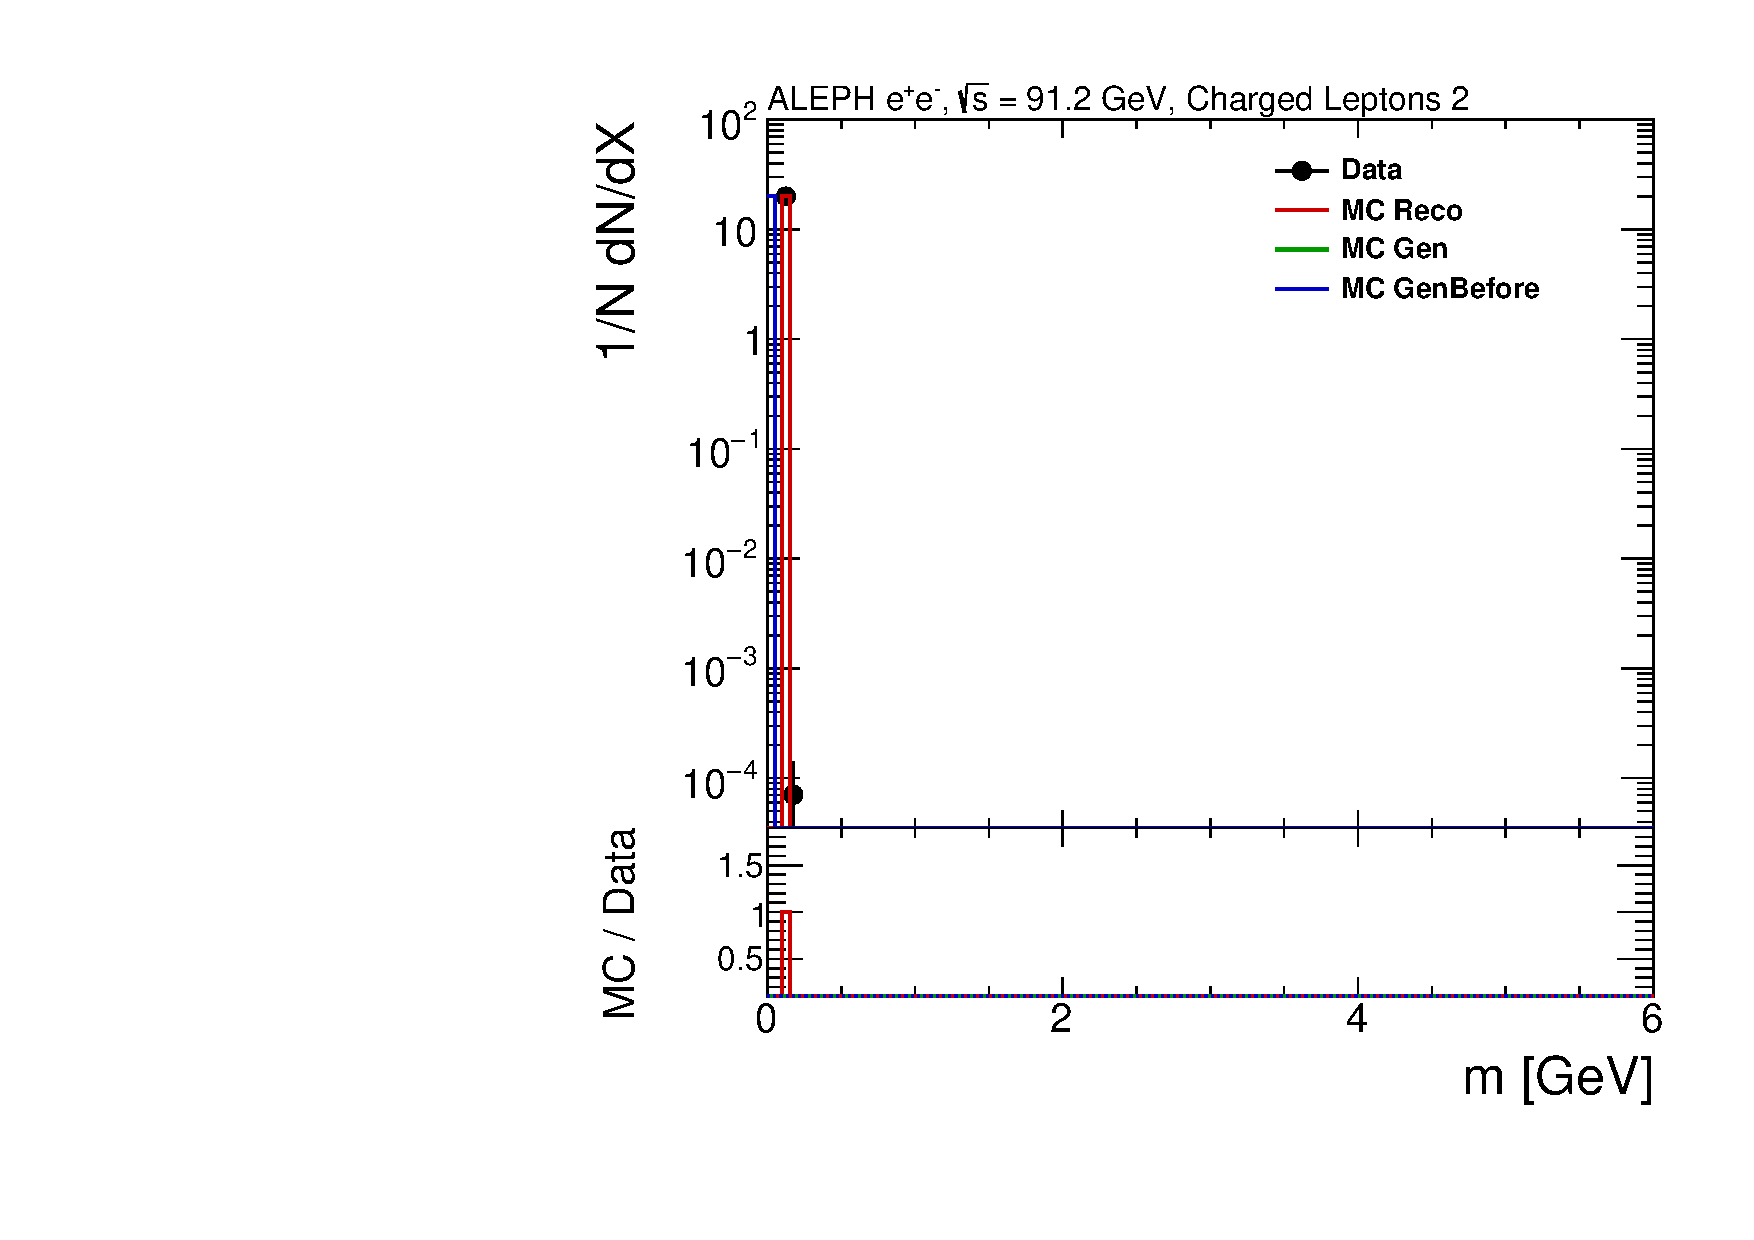
\includegraphics[width=0.325\textwidth]{../Studies/PreliminaryResult/2026-02-17_thrust_iter5/pwflag_kinematics/pwflag2_mass.pdf}
\caption{Complete \texttt{pwflag}=2 kinematic set.}
\label{fig:pwflag2_full}
\end{figure}

\noindent
Figure~\ref{fig:pwflag2_full} presents the second charged-lepton category, providing a direct
cross-check of category-dependent acceptance and momentum-shape modeling. This category probes
objects with different subdetector signatures than Fig.~\ref{fig:pwflag1_full}, so agreement
here confirms that lepton-category partitioning does not induce a hidden detector asymmetry in
the thrust inputs. The high-$p_T$ and high-energy tails are monitored explicitly because even a
small mismodeling there can project onto endpoint thrust bins.

\begin{figure}[t!]
\centering
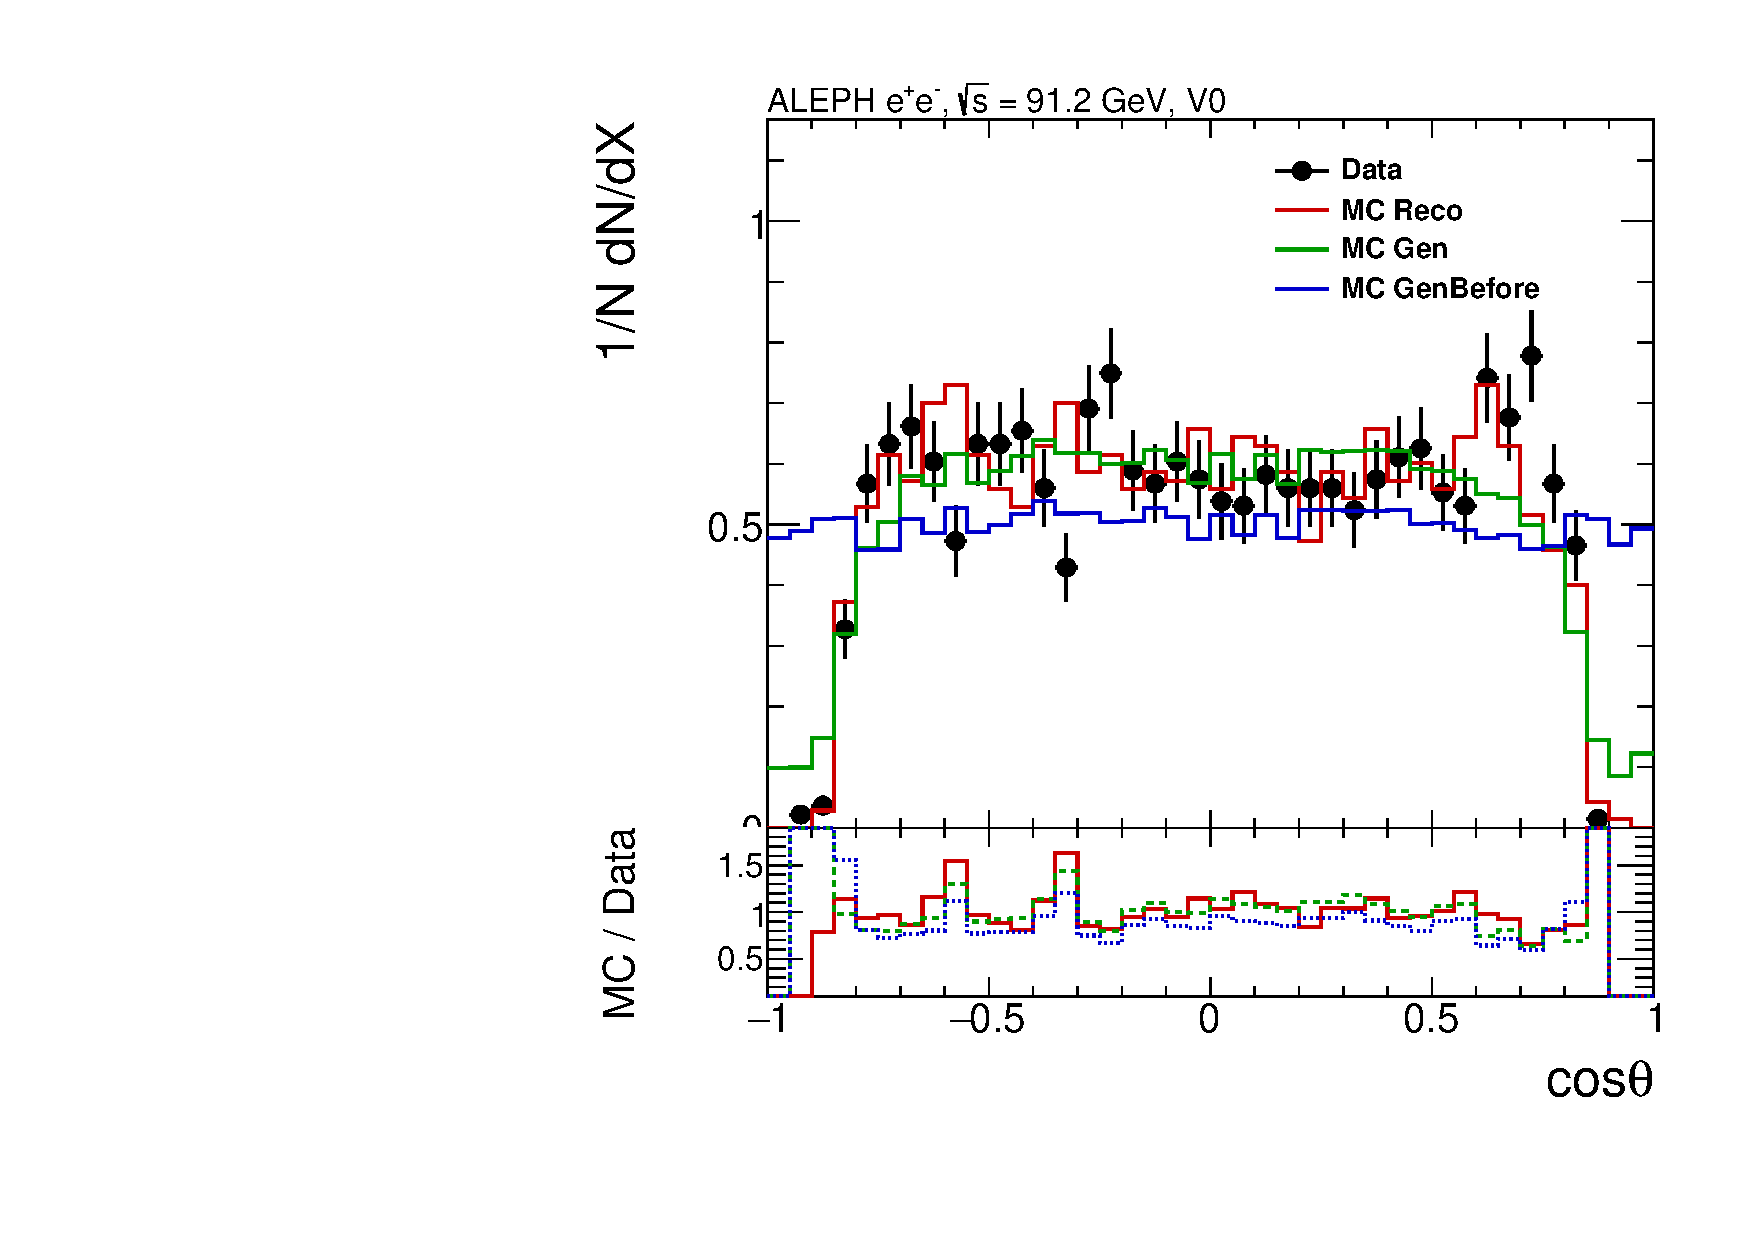
\includegraphics[width=0.325\textwidth]{../Studies/PreliminaryResult/2026-02-17_thrust_iter5/pwflag_kinematics/pwflag3_cosTheta.pdf}
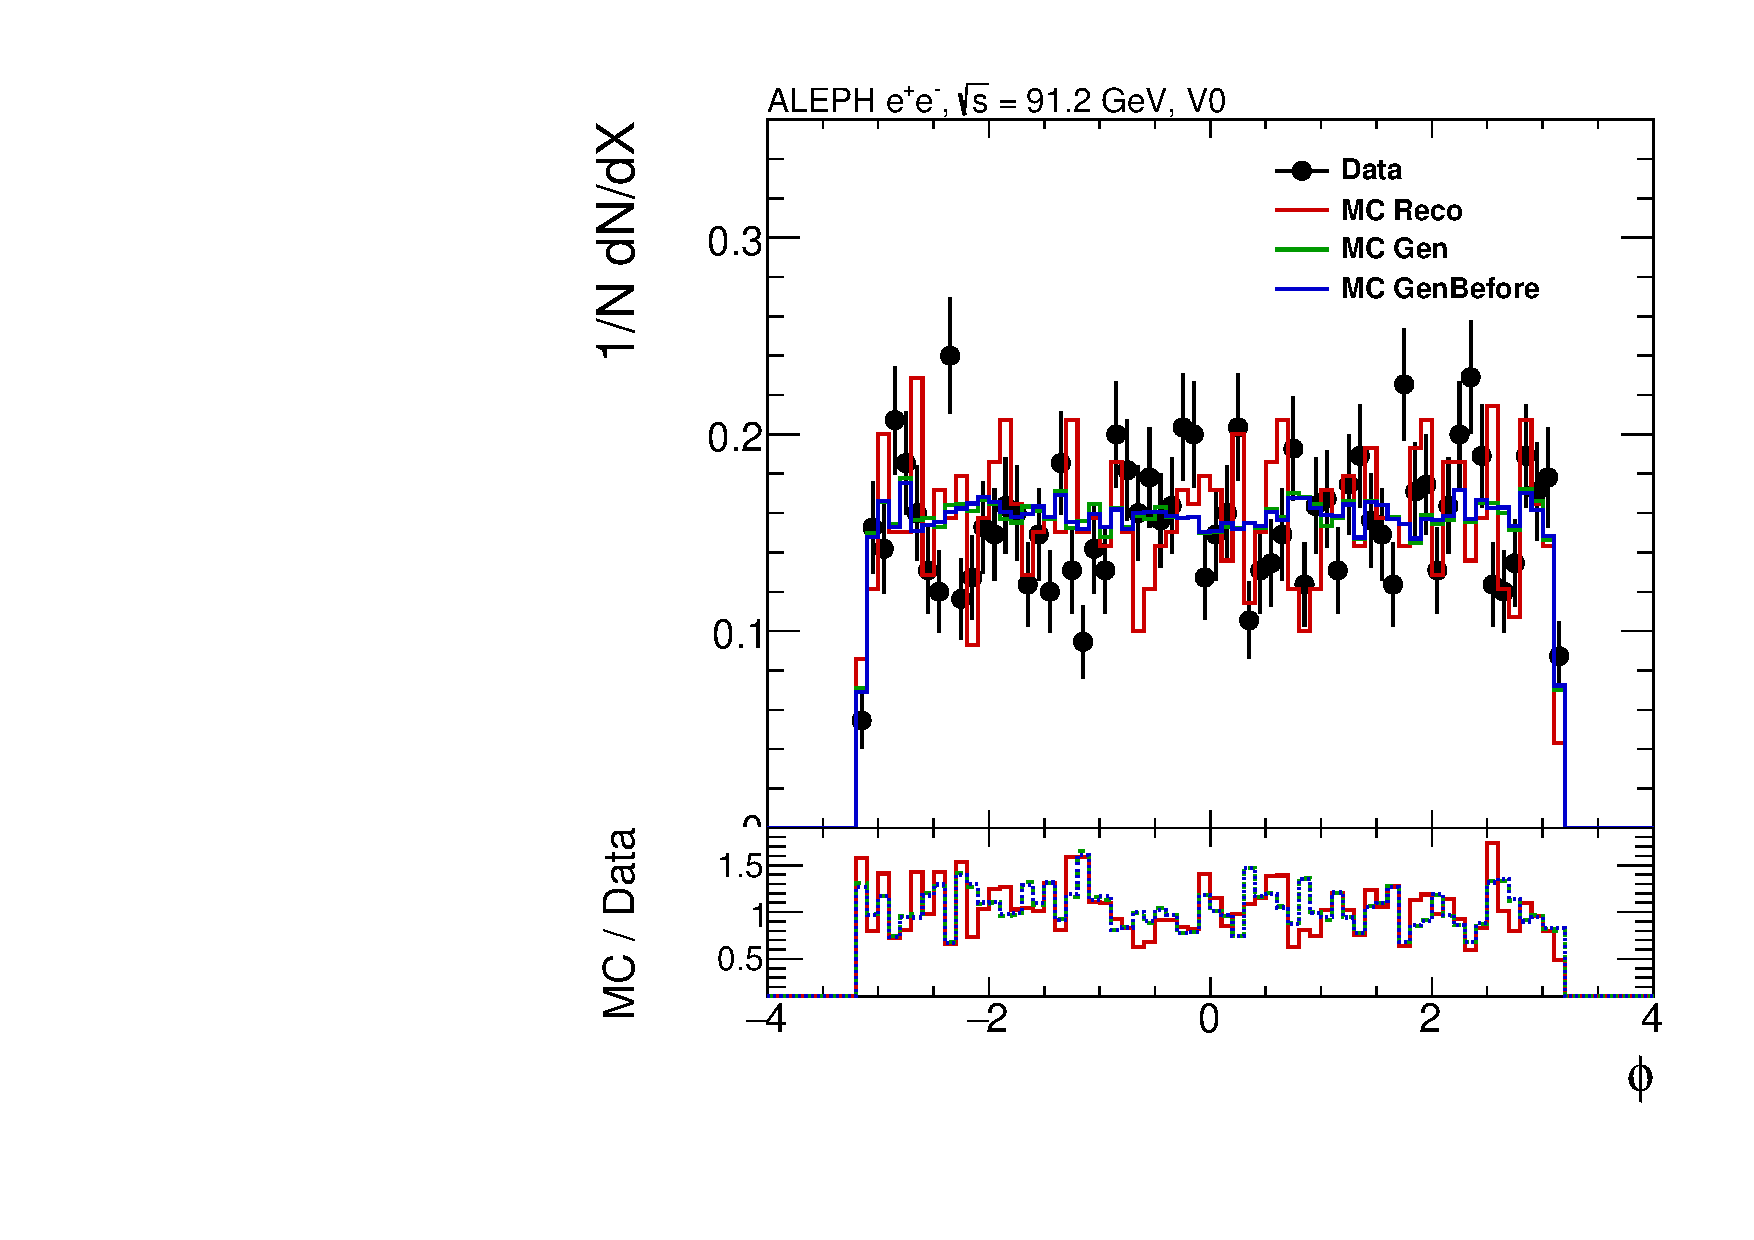
\includegraphics[width=0.325\textwidth]{../Studies/PreliminaryResult/2026-02-17_thrust_iter5/pwflag_kinematics/pwflag3_phi.pdf}
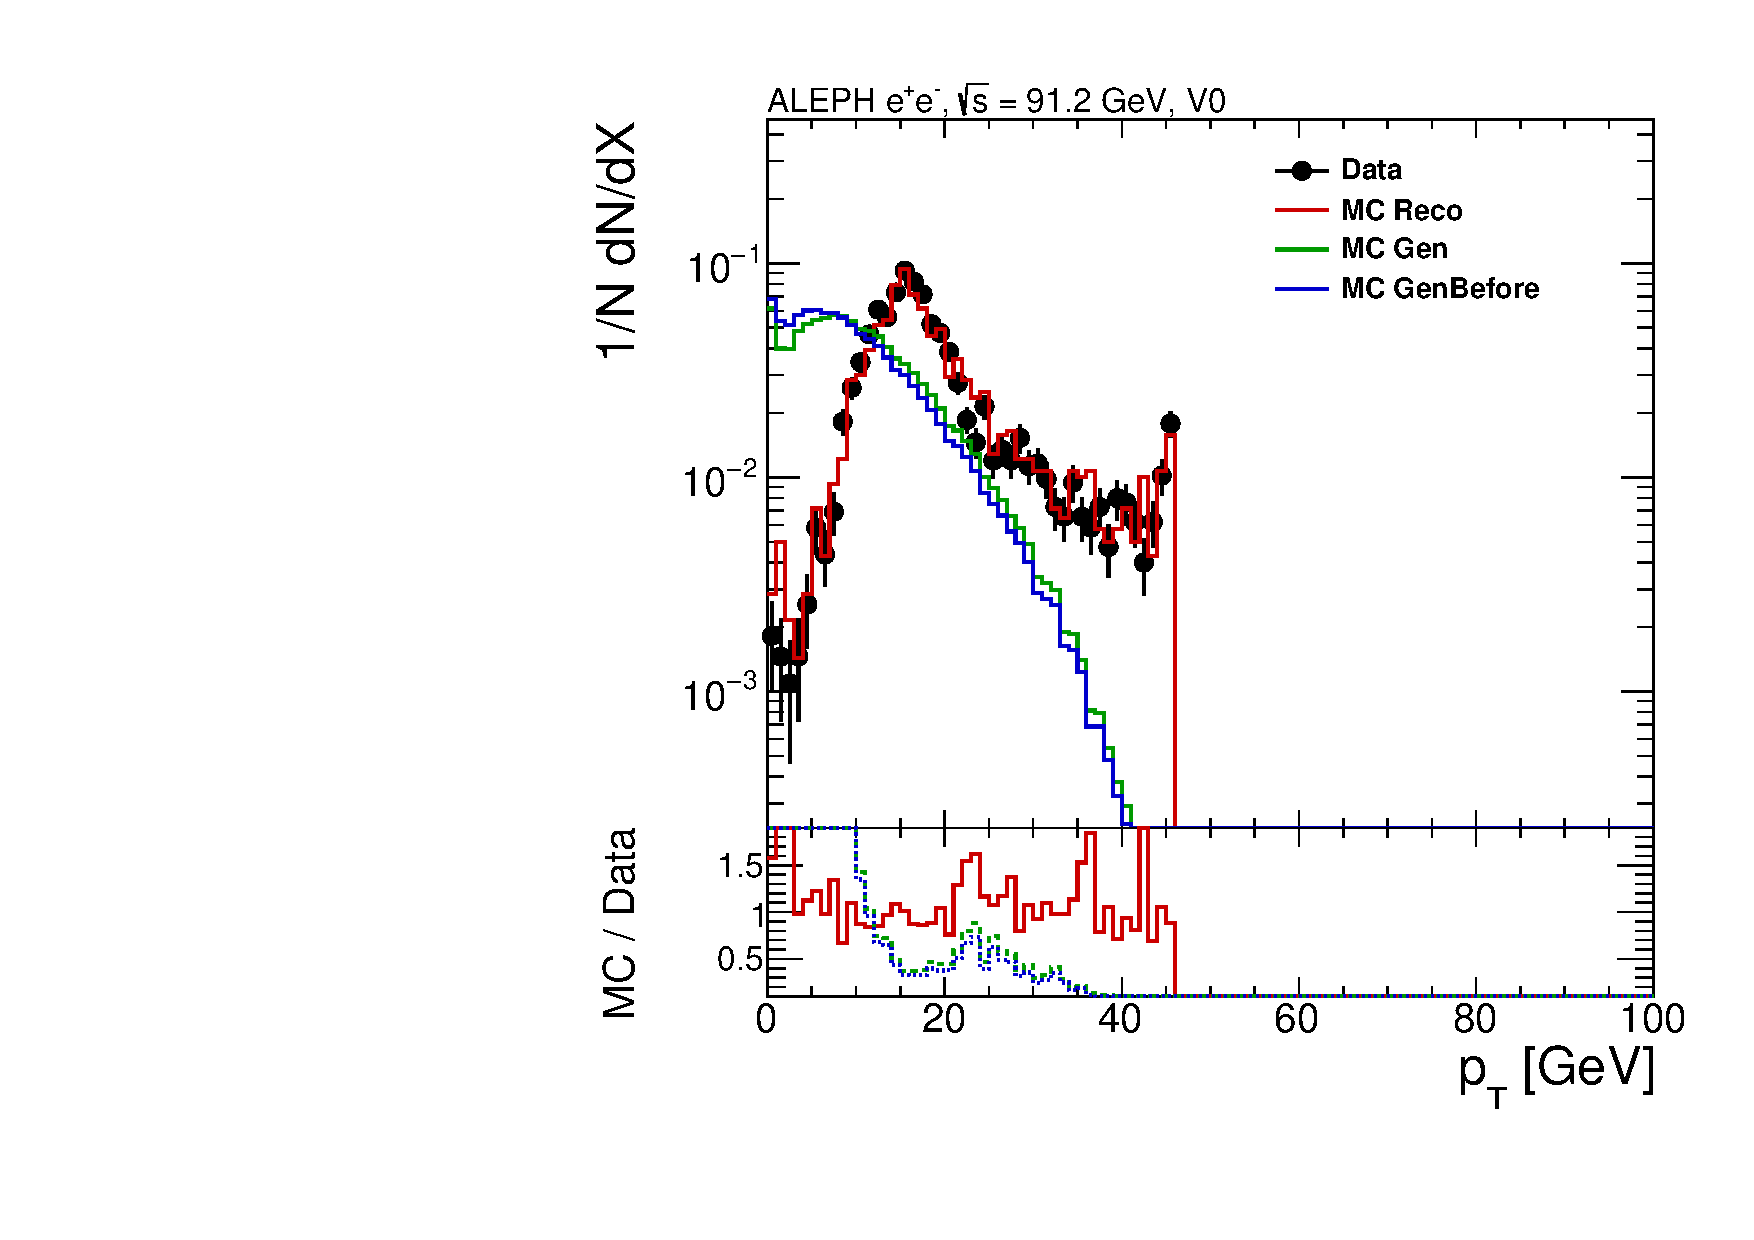
\includegraphics[width=0.325\textwidth]{../Studies/PreliminaryResult/2026-02-17_thrust_iter5/pwflag_kinematics/pwflag3_pt.pdf}
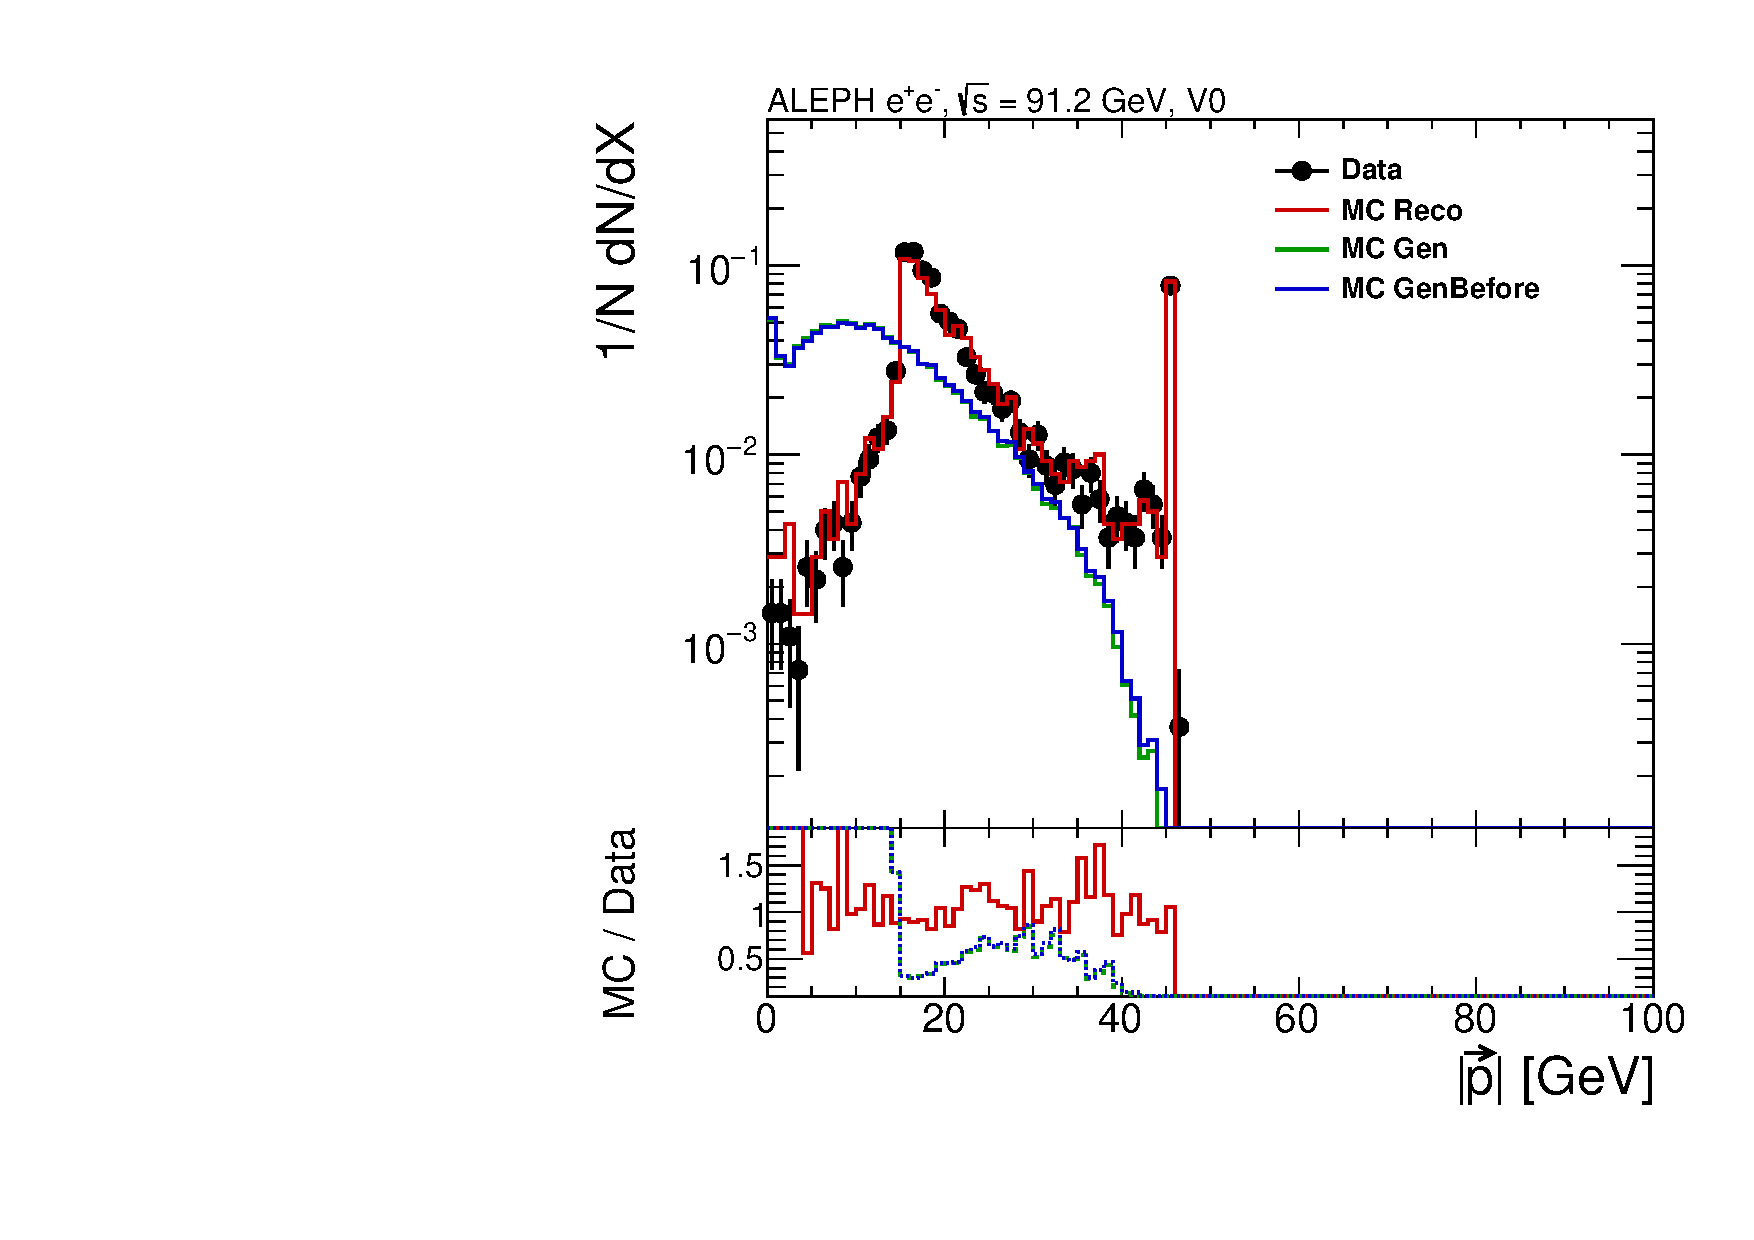
\includegraphics[width=0.325\textwidth]{../Studies/PreliminaryResult/2026-02-17_thrust_iter5/pwflag_kinematics/pwflag3_pmag.pdf}
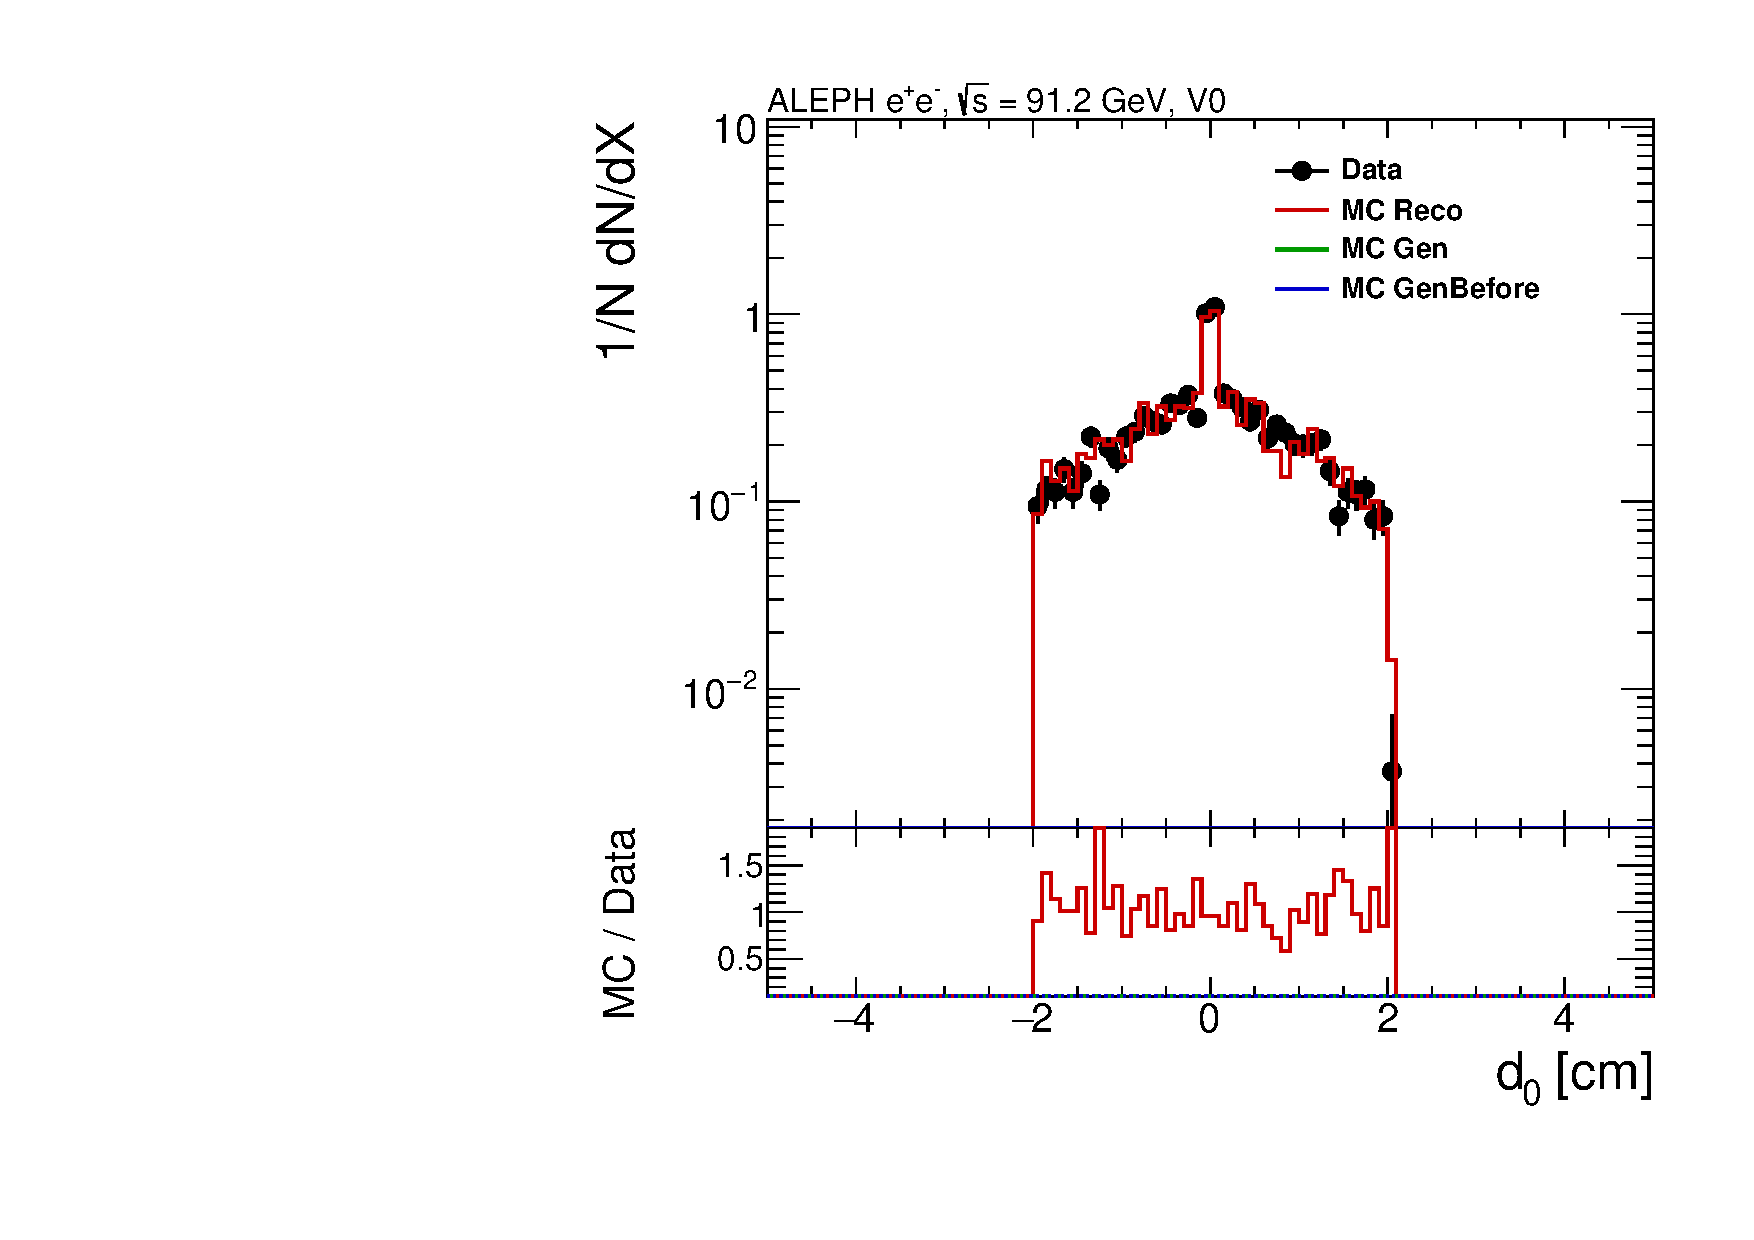
\includegraphics[width=0.325\textwidth]{../Studies/PreliminaryResult/2026-02-17_thrust_iter5/pwflag_kinematics/pwflag3_d0.pdf}
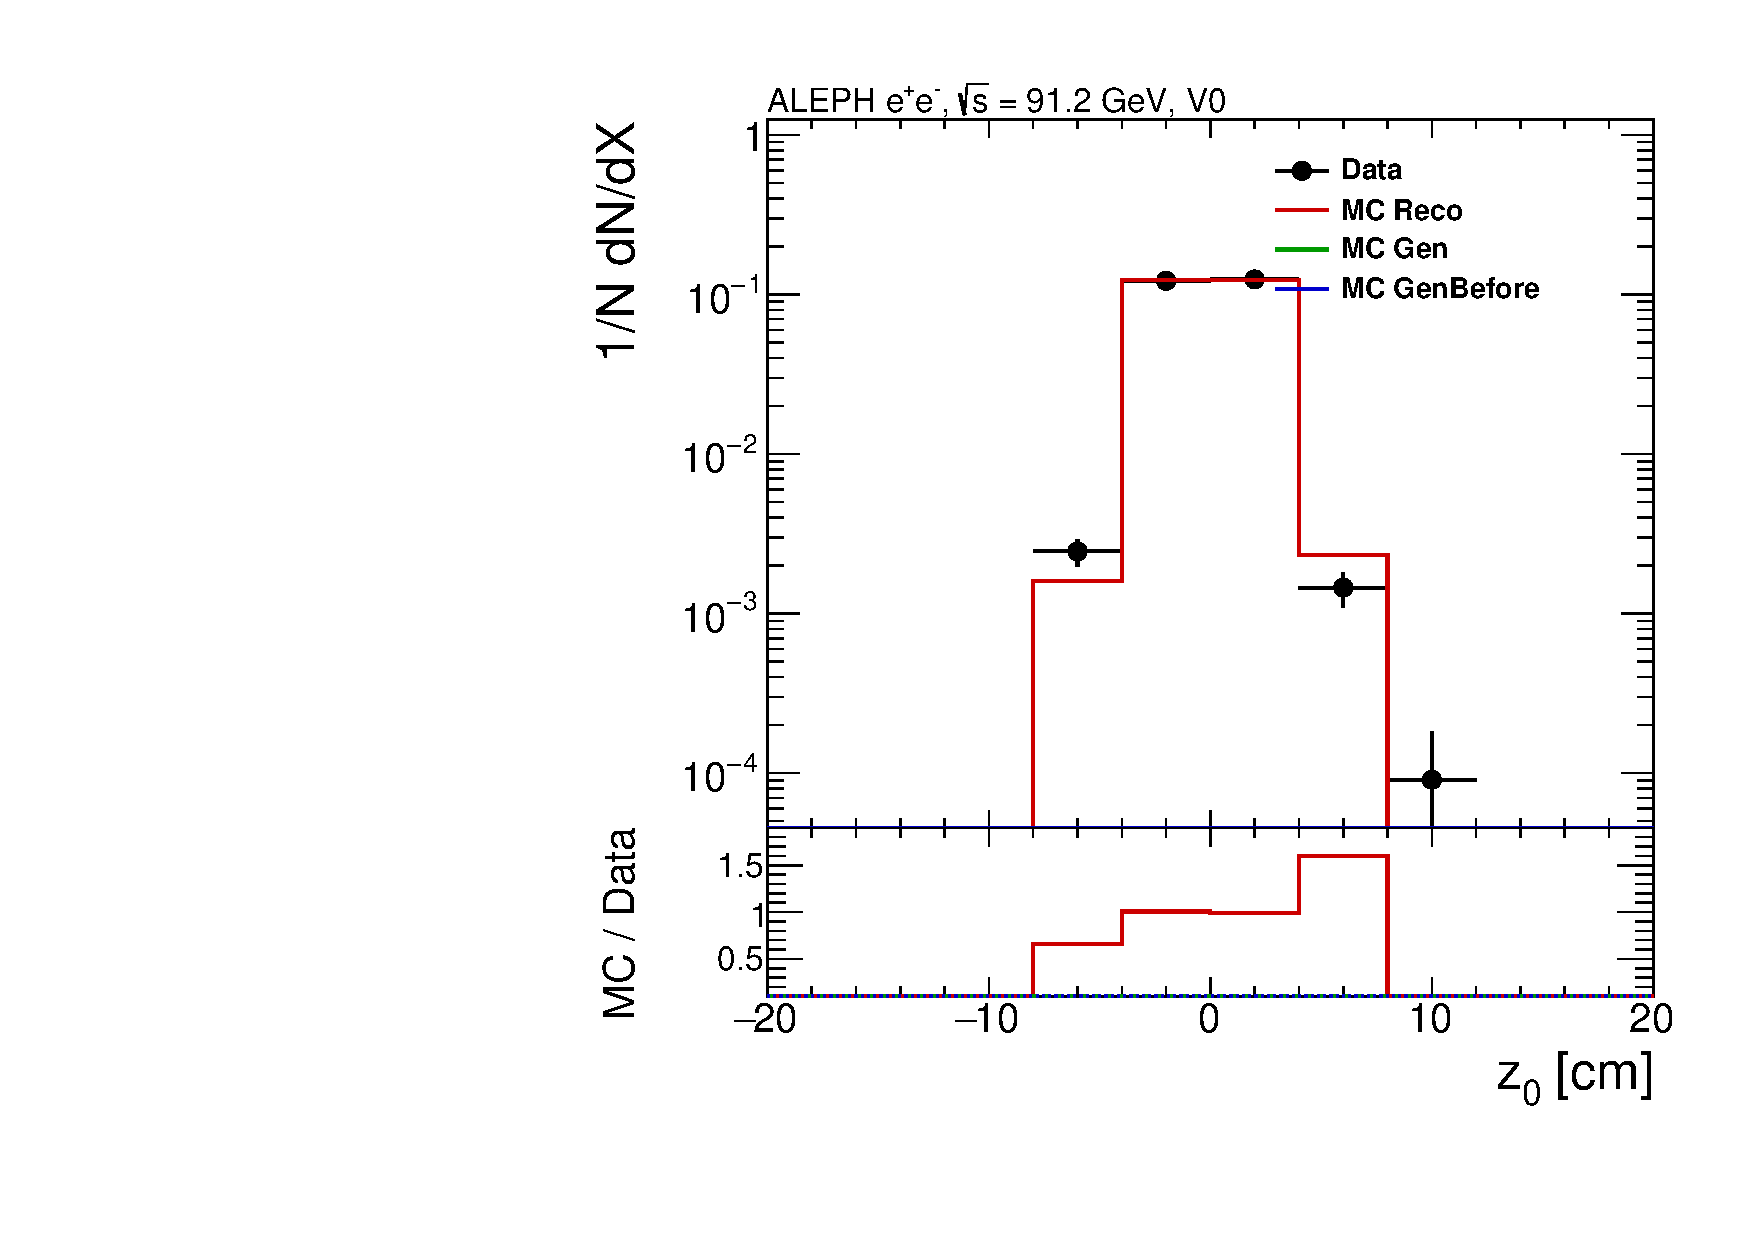
\includegraphics[width=0.325\textwidth]{../Studies/PreliminaryResult/2026-02-17_thrust_iter5/pwflag_kinematics/pwflag3_z0.pdf}
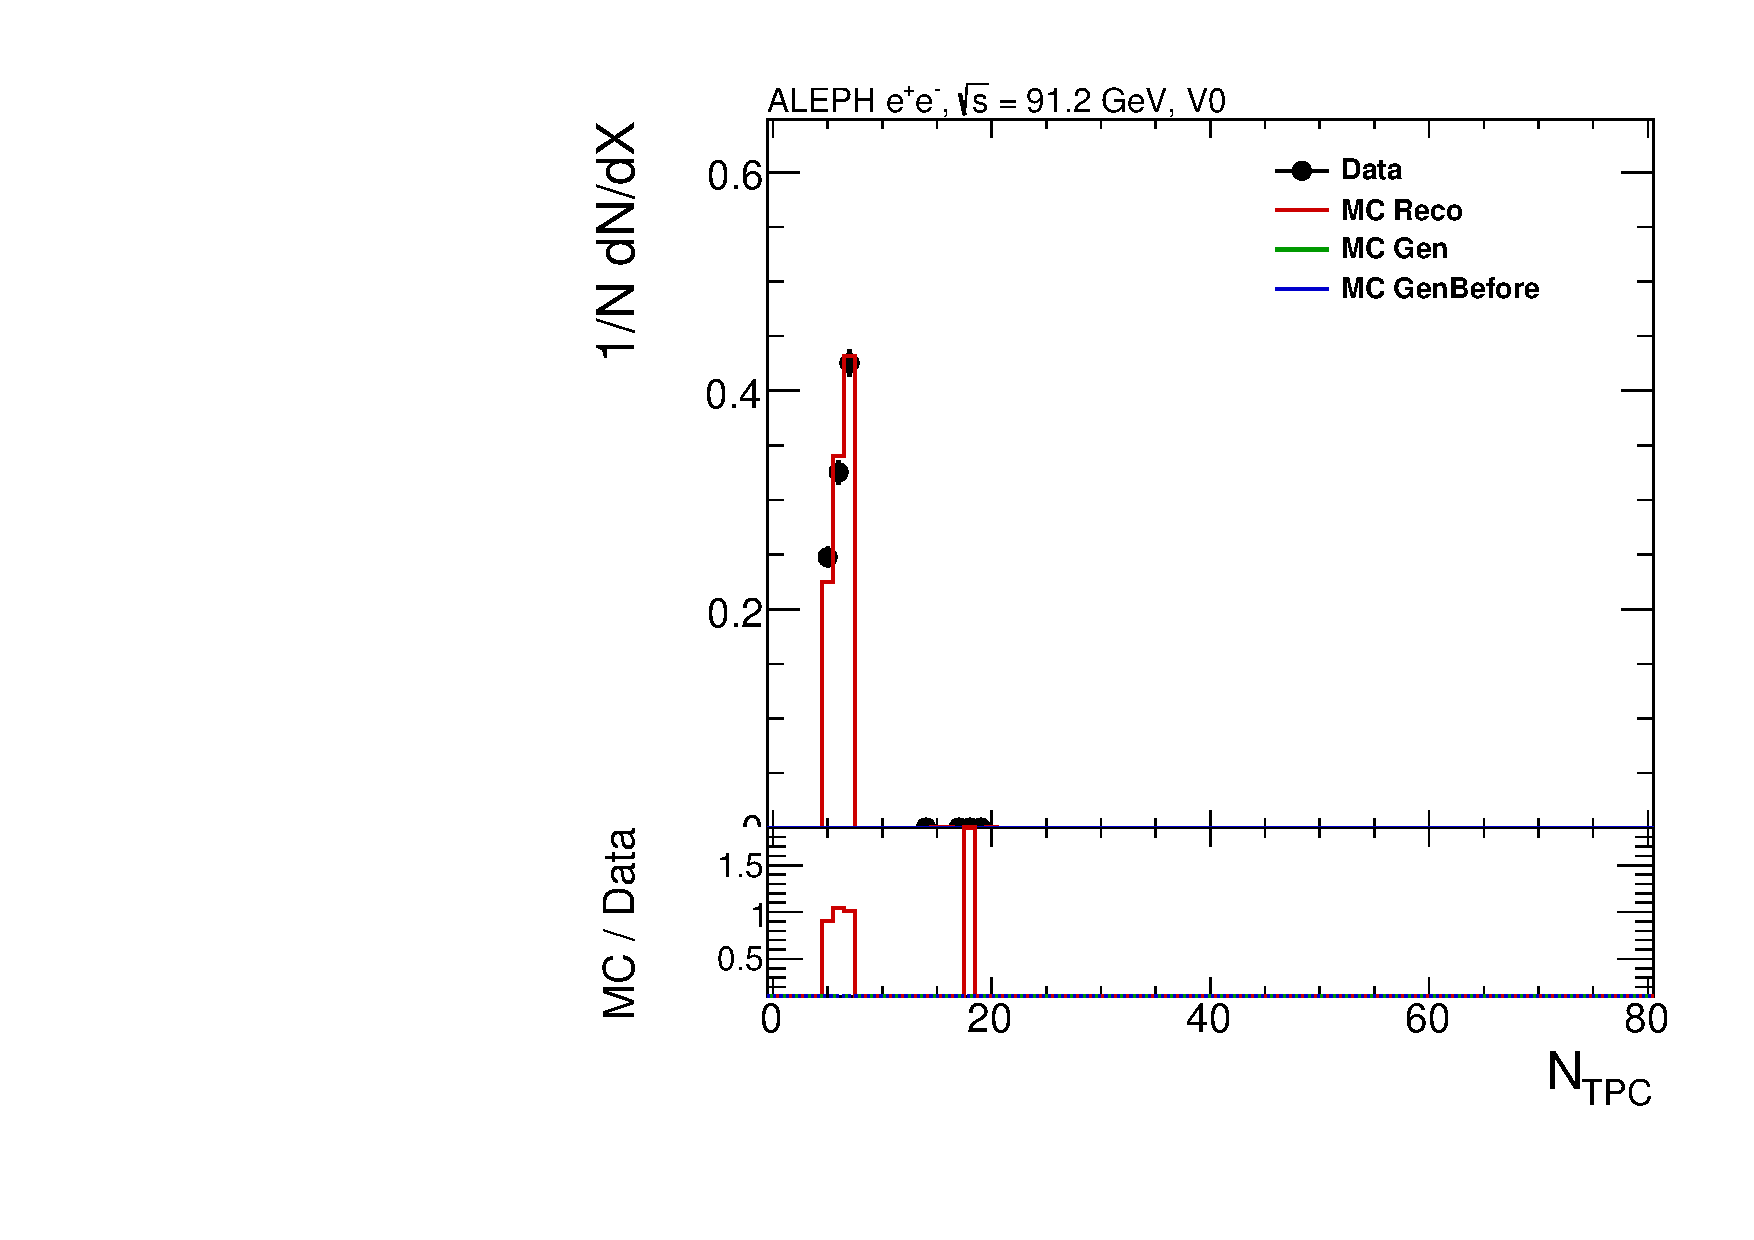
\includegraphics[width=0.325\textwidth]{../Studies/PreliminaryResult/2026-02-17_thrust_iter5/pwflag_kinematics/pwflag3_ntpc.pdf}
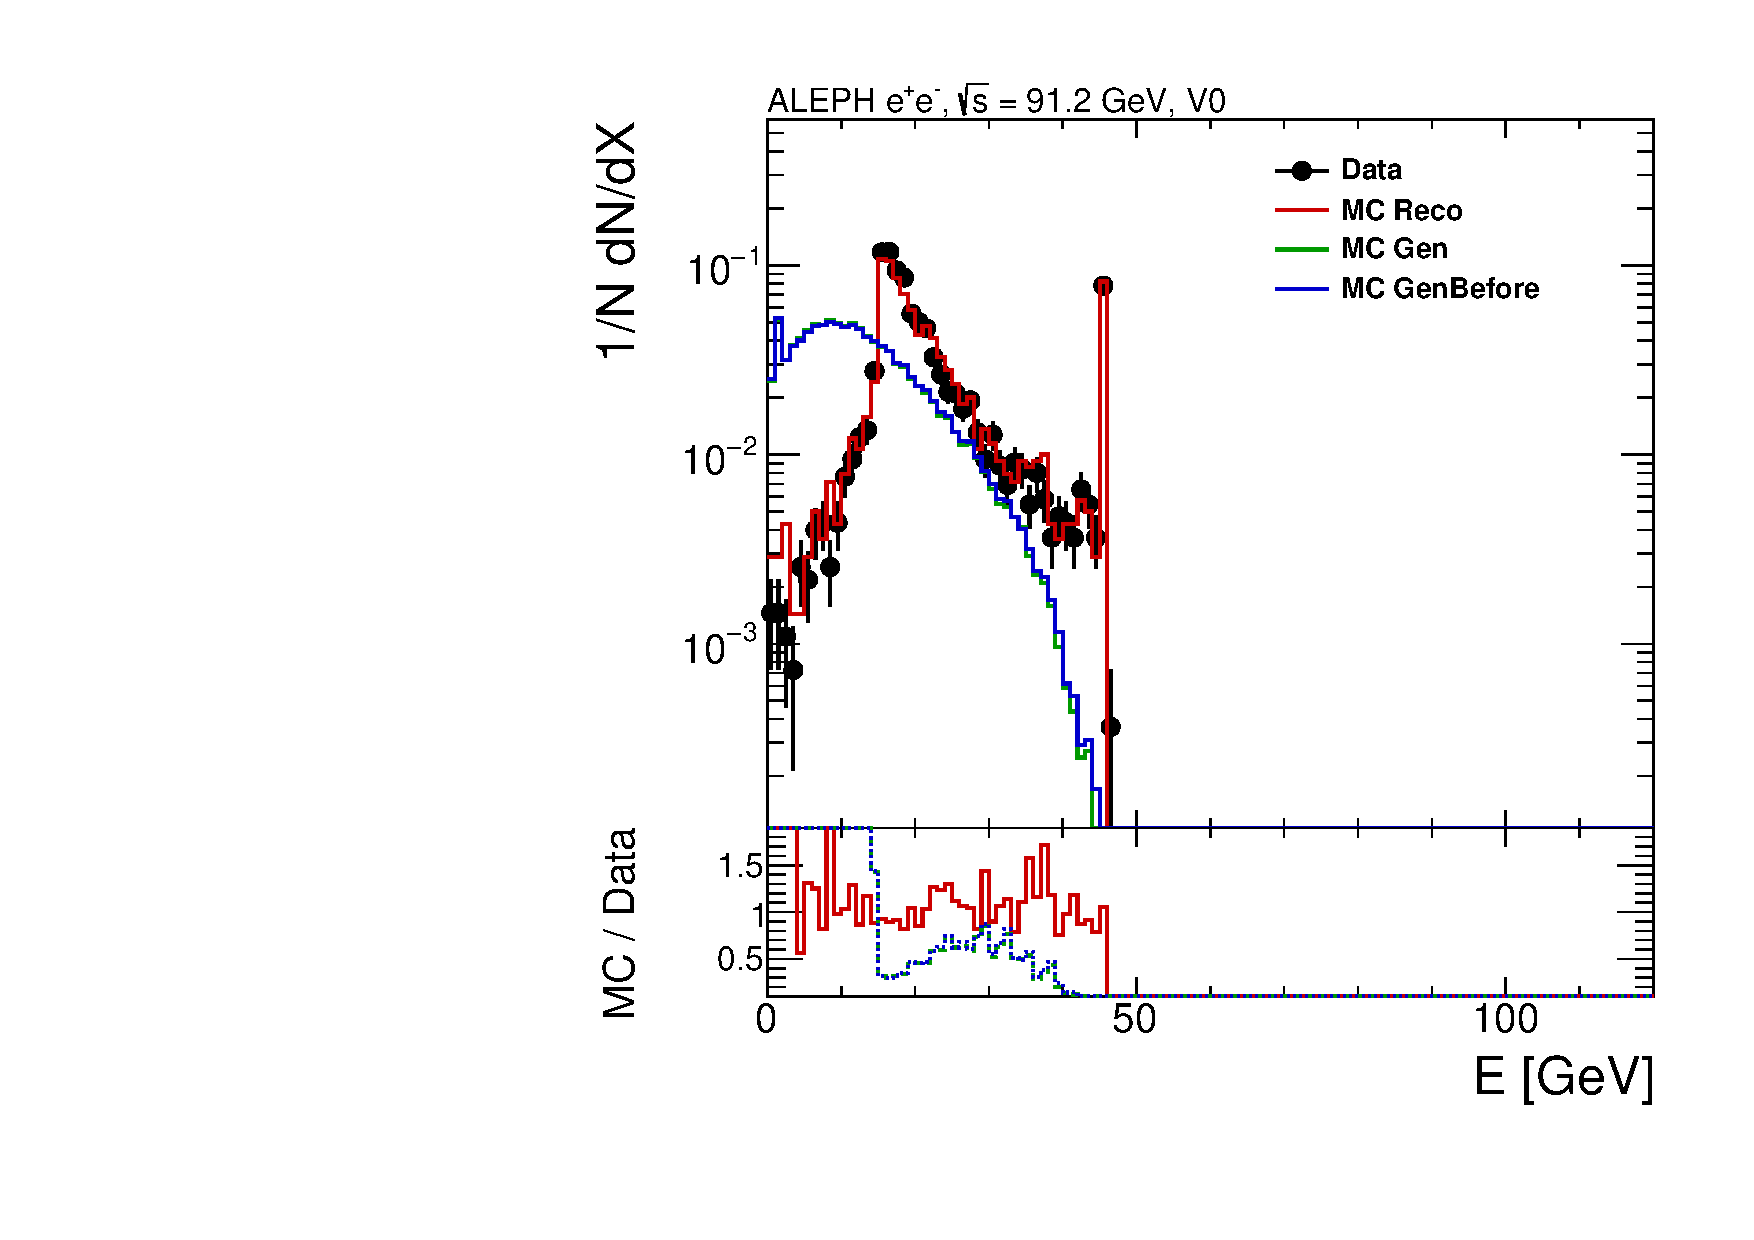
\includegraphics[width=0.325\textwidth]{../Studies/PreliminaryResult/2026-02-17_thrust_iter5/pwflag_kinematics/pwflag3_energy.pdf}
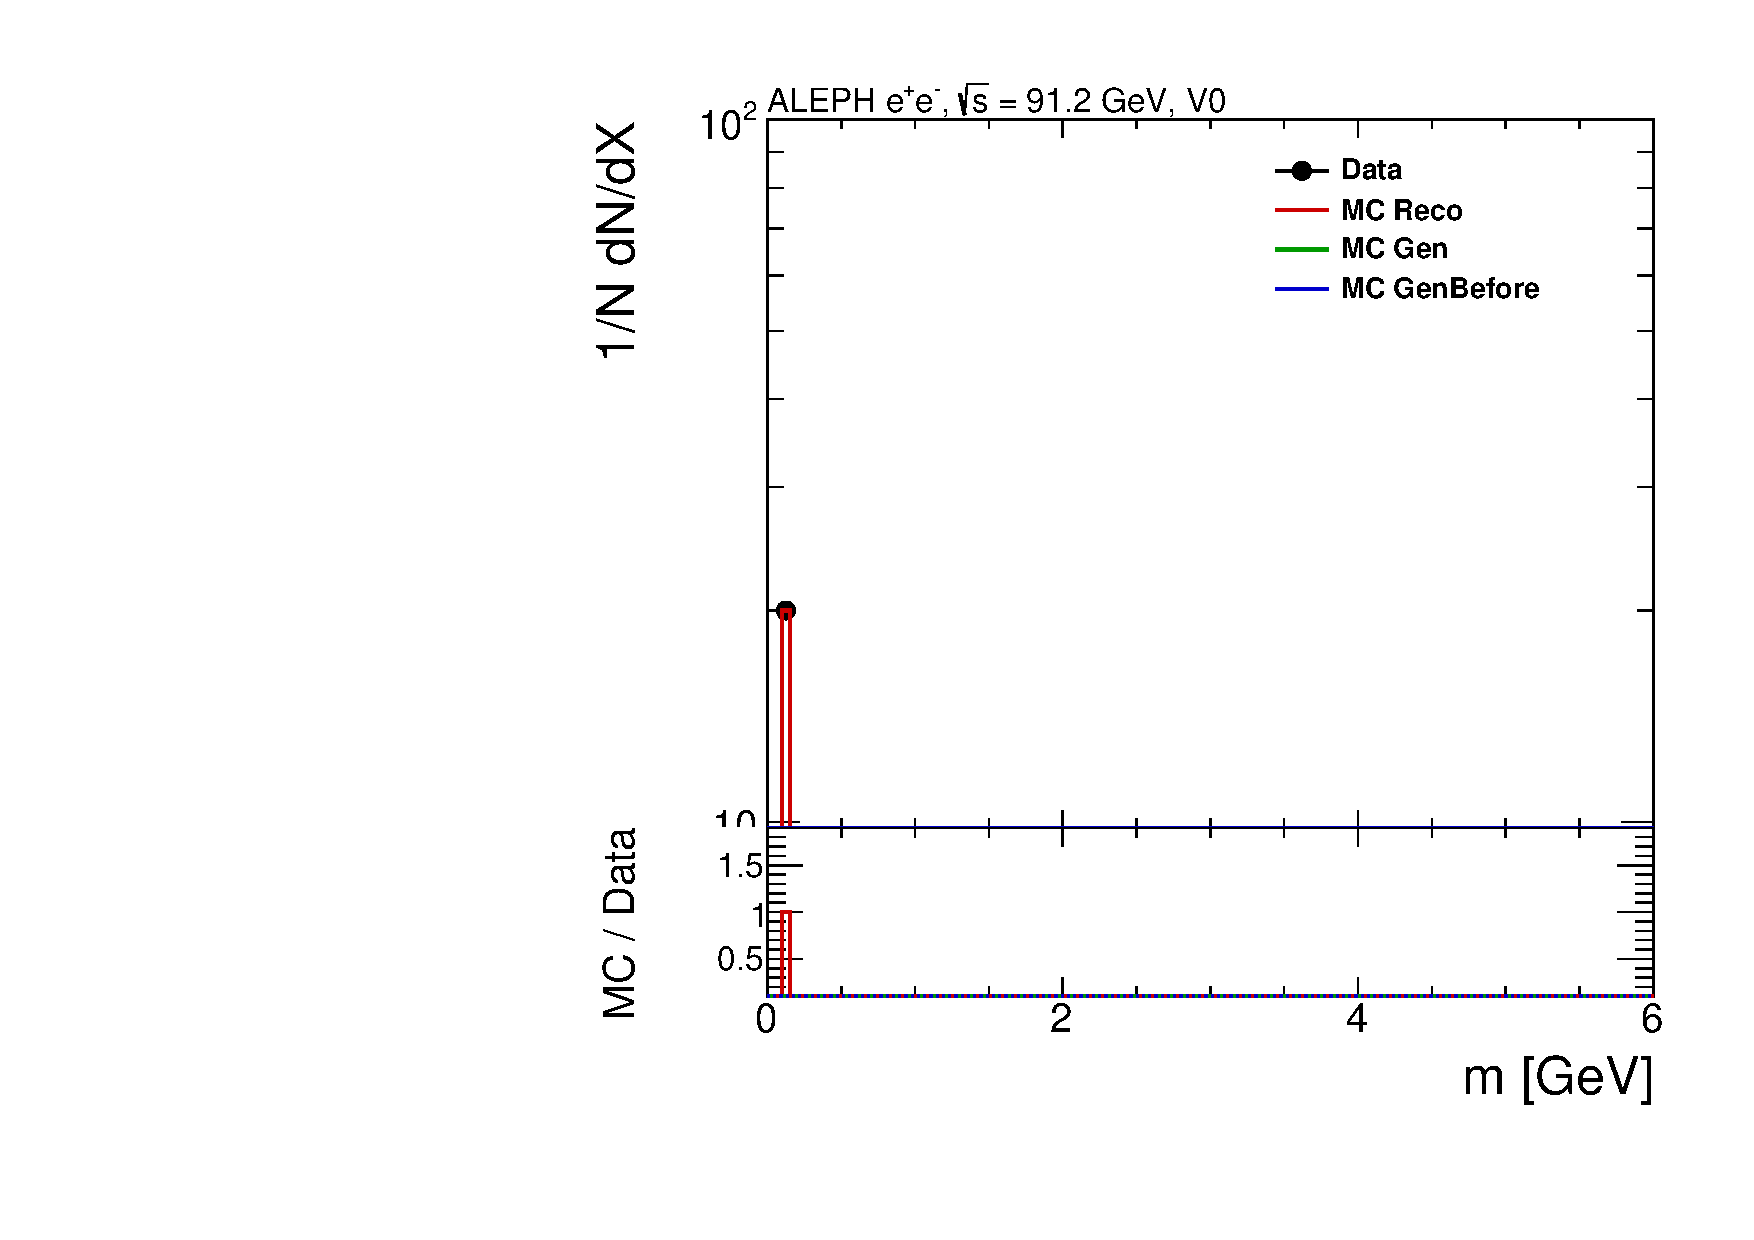
\includegraphics[width=0.325\textwidth]{../Studies/PreliminaryResult/2026-02-17_thrust_iter5/pwflag_kinematics/pwflag3_mass.pdf}
\caption{Complete \texttt{pwflag}=3 kinematic set.}
\label{fig:pwflag3_full}
\end{figure}

\noindent
Figure~\ref{fig:pwflag3_full} begins the neutral-object categories, where angular and energy
modeling are especially relevant for visible-energy flow in thrust reconstruction. For this
category, the energy spectrum and angular acceptance are the primary physics handles for event
shape modeling, while the track-like quantities provide consistency checks of the archived object
classification. Agreement in this panel supports a controlled transfer of neutral energy flow into
the unfolded thrust response.

\begin{figure}[t!]
\centering
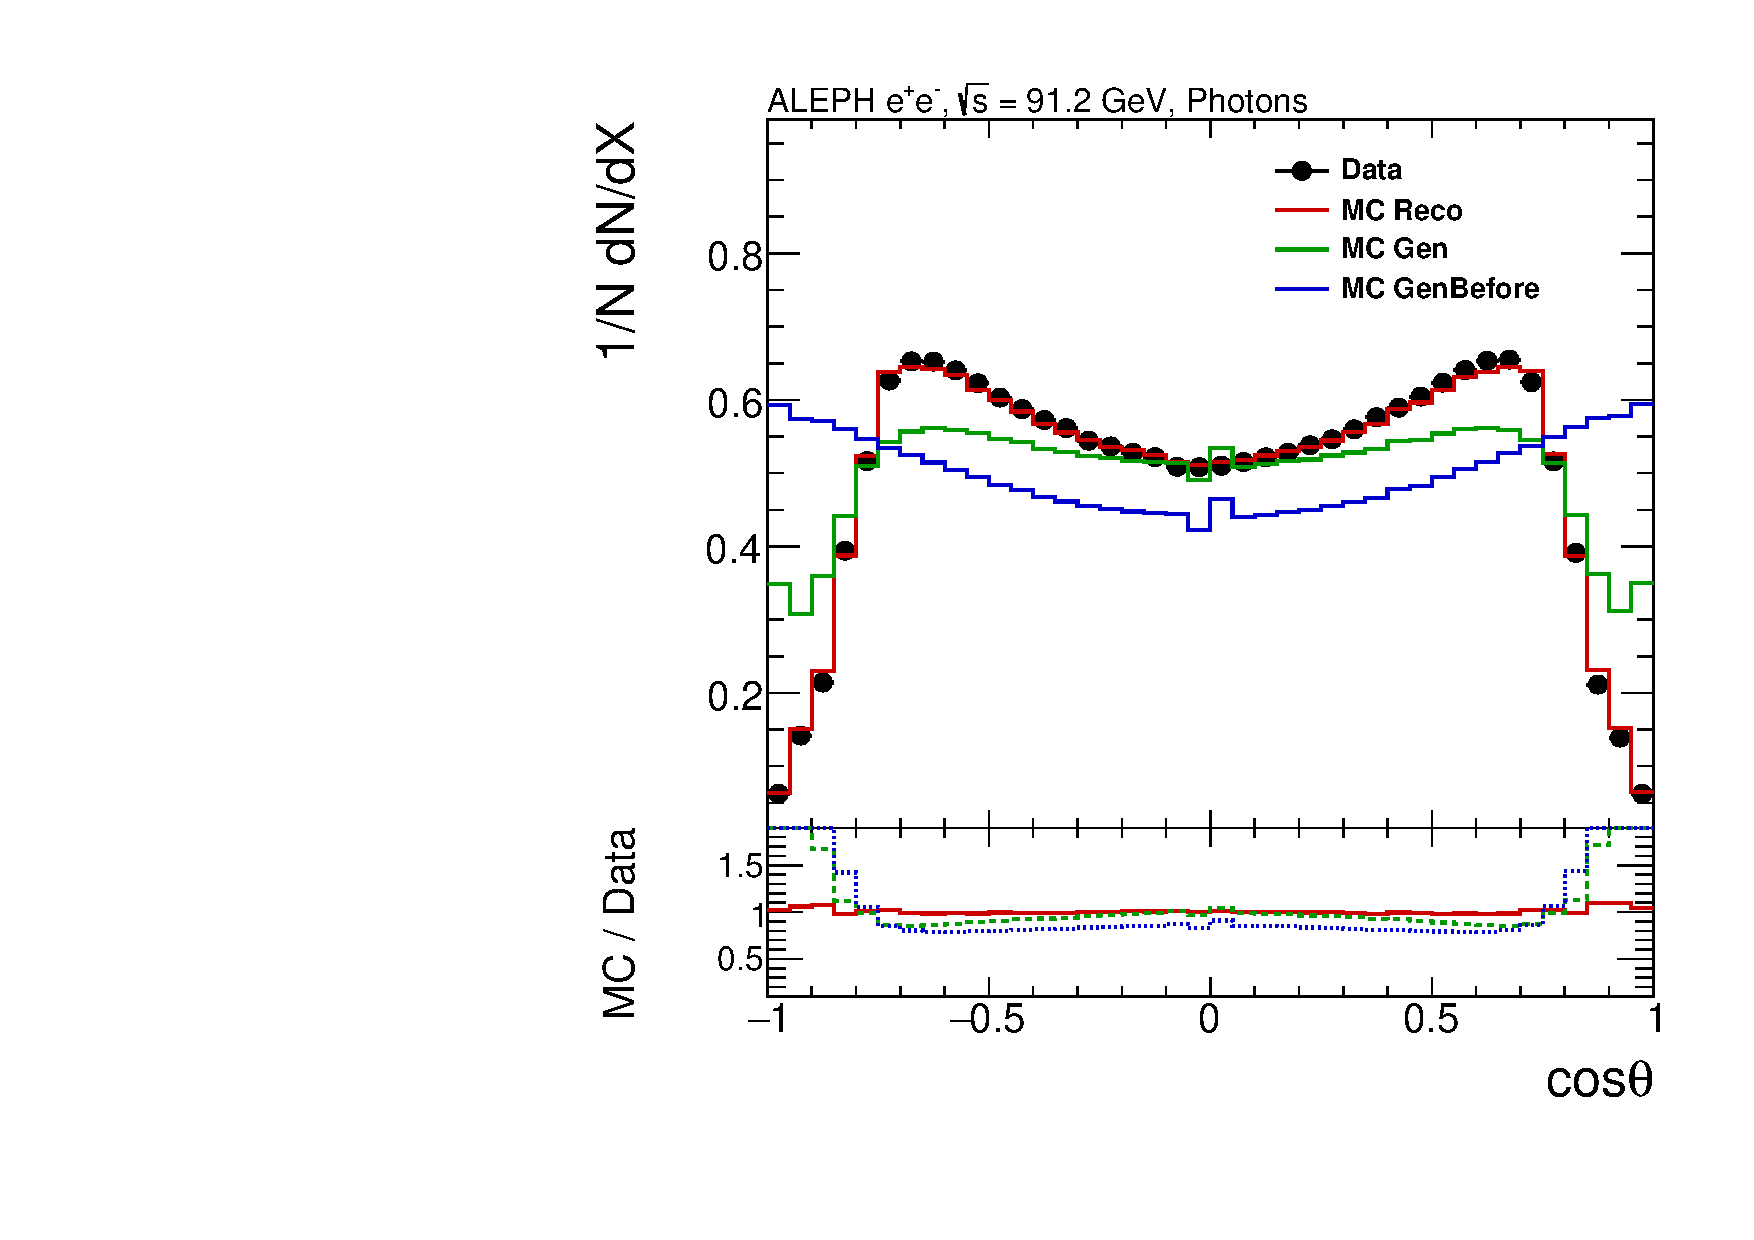
\includegraphics[width=0.325\textwidth]{../Studies/PreliminaryResult/2026-02-17_thrust_iter5/pwflag_kinematics/pwflag4_cosTheta.pdf}
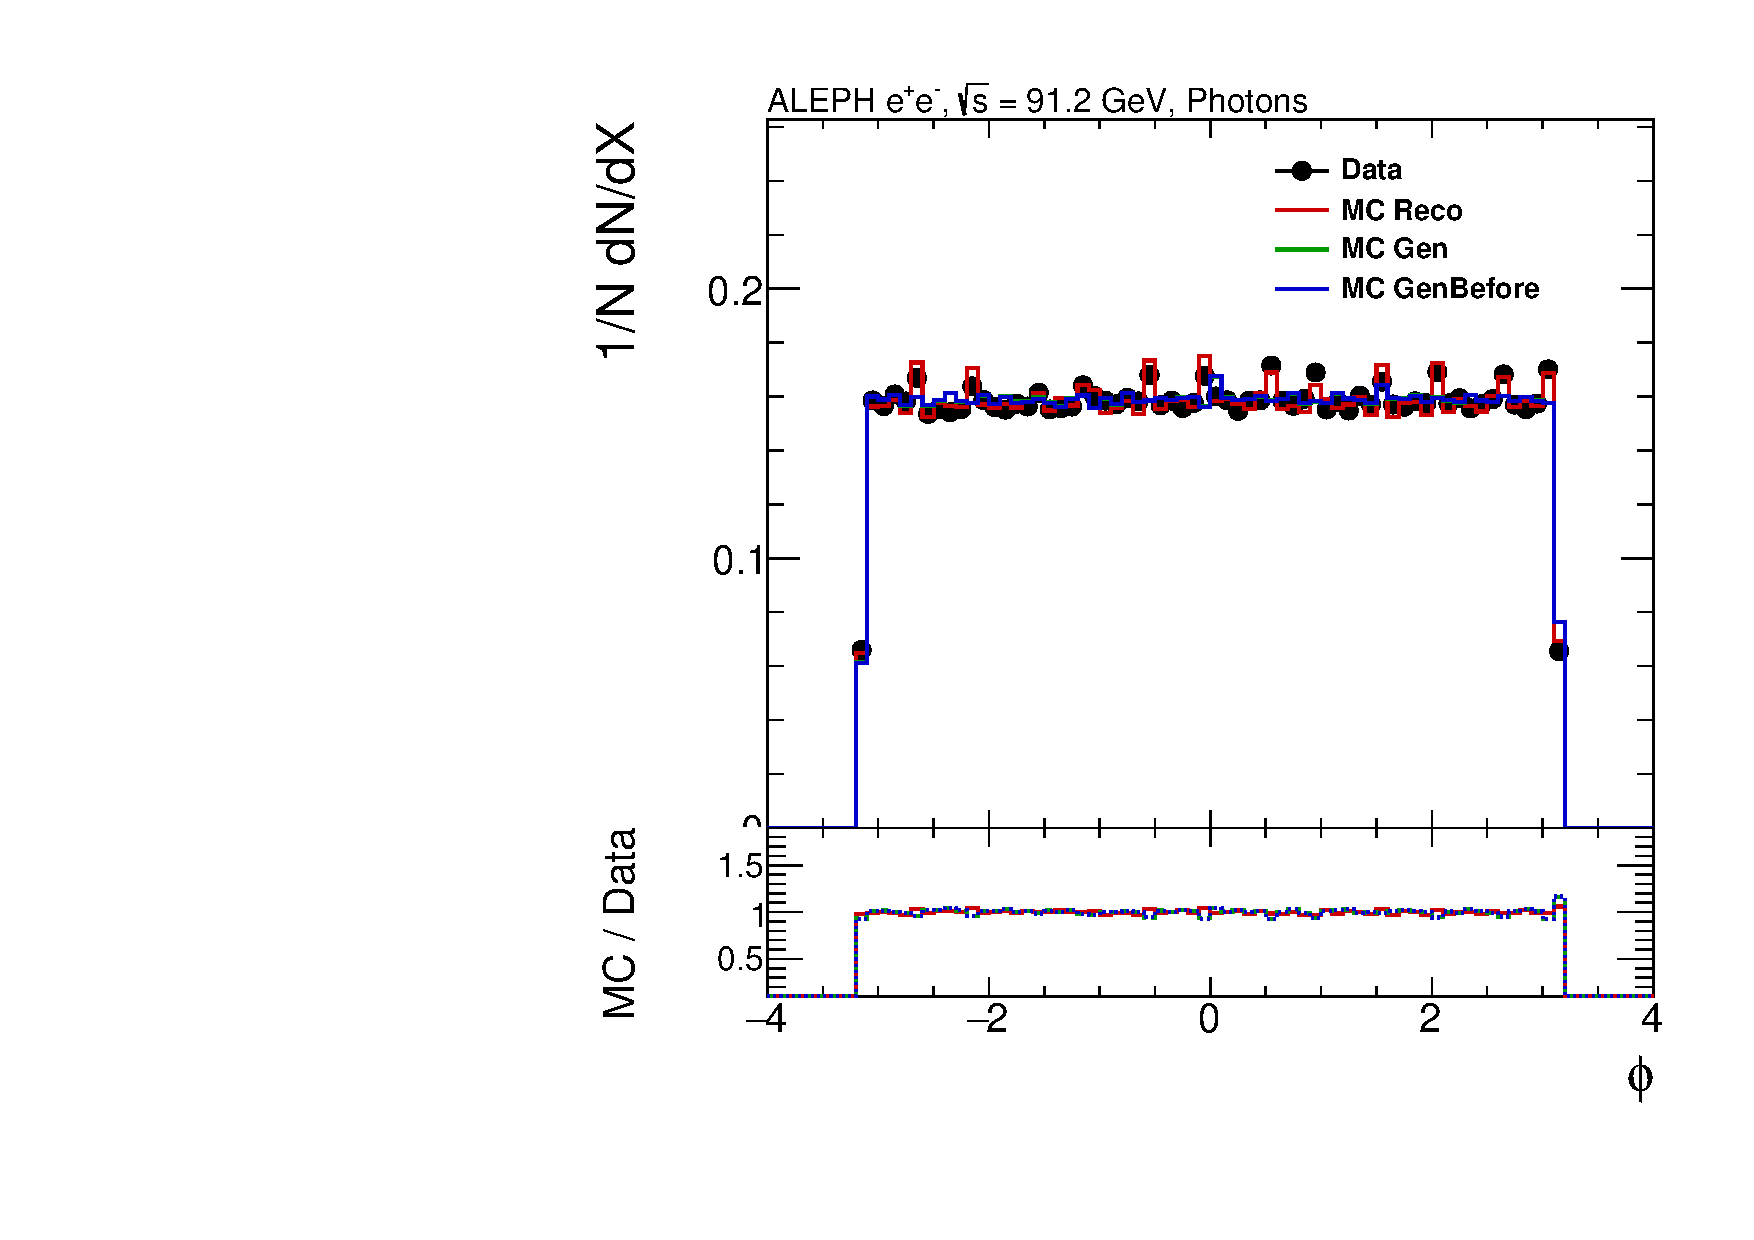
\includegraphics[width=0.325\textwidth]{../Studies/PreliminaryResult/2026-02-17_thrust_iter5/pwflag_kinematics/pwflag4_phi.pdf}
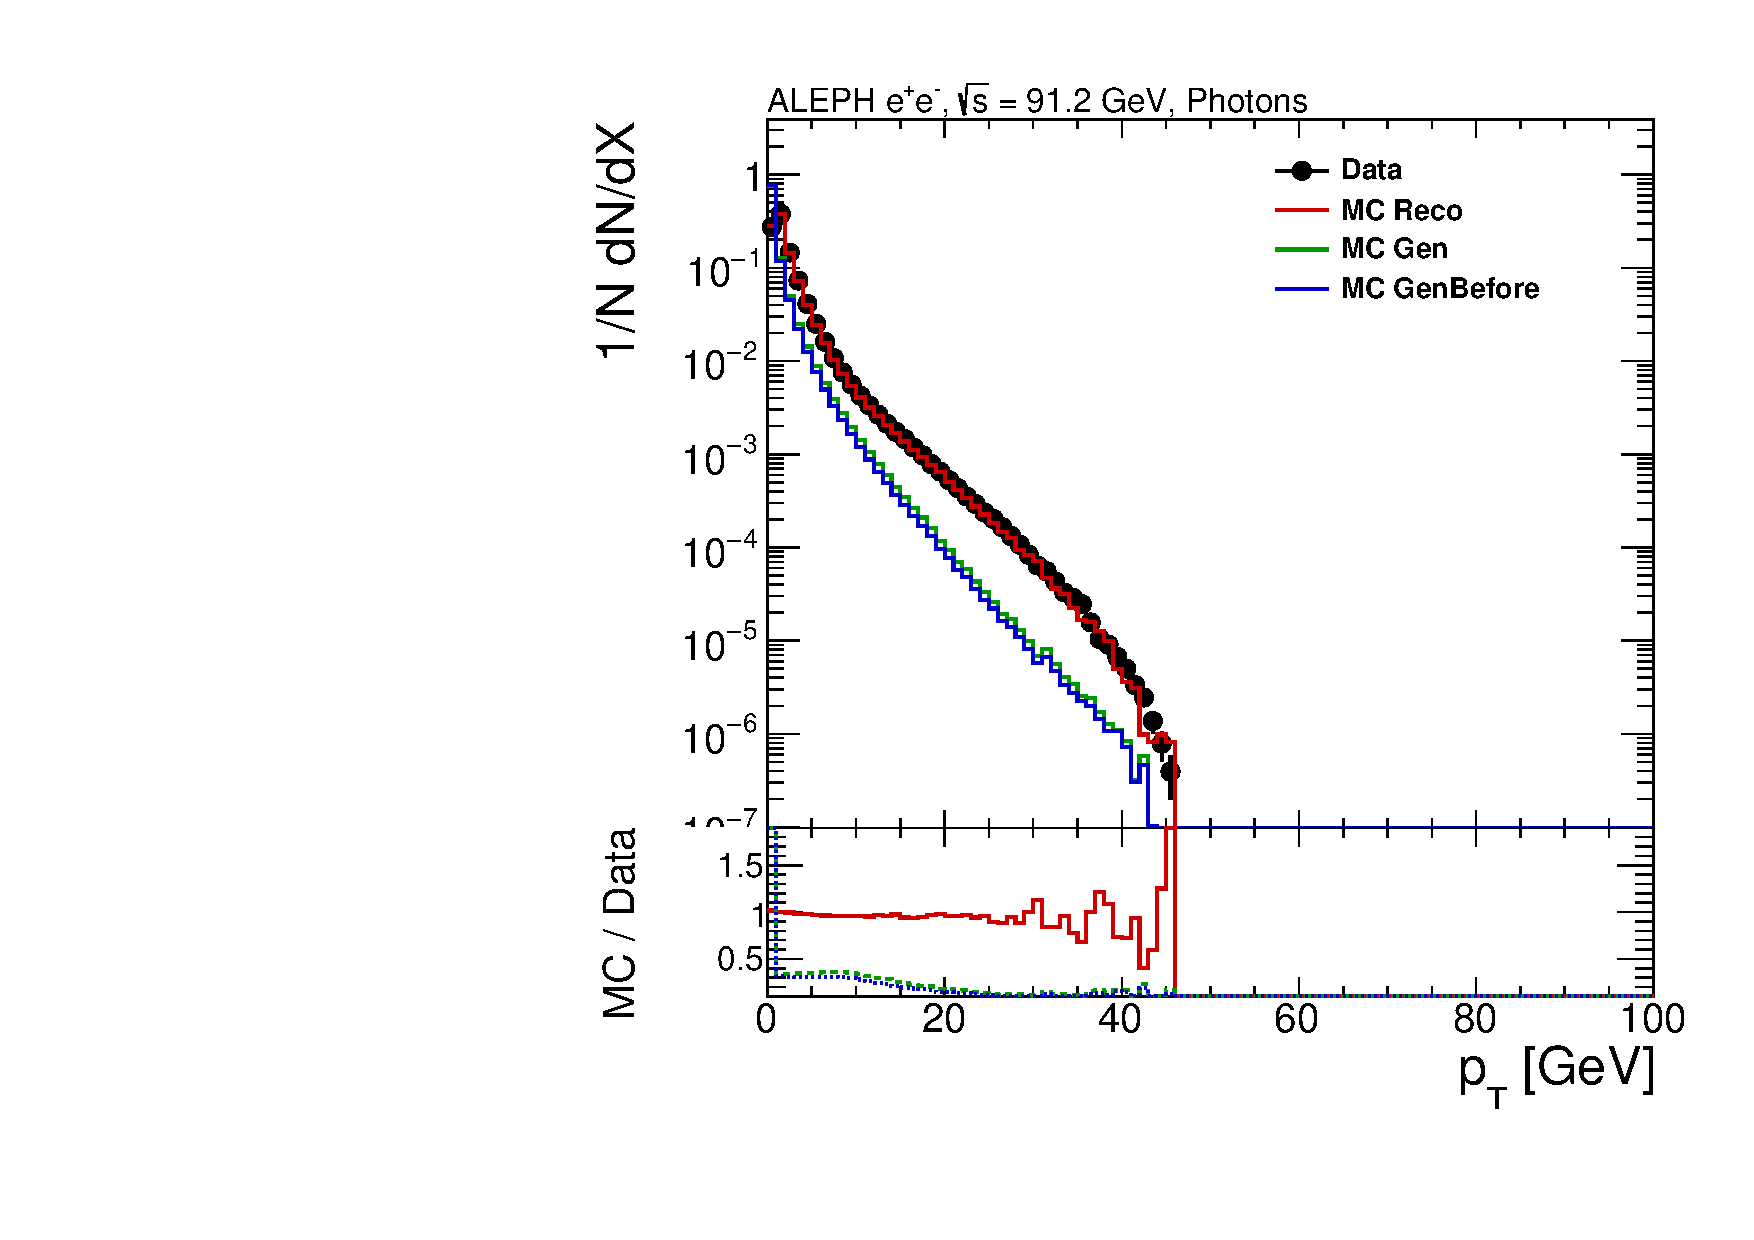
\includegraphics[width=0.325\textwidth]{../Studies/PreliminaryResult/2026-02-17_thrust_iter5/pwflag_kinematics/pwflag4_pt.pdf}
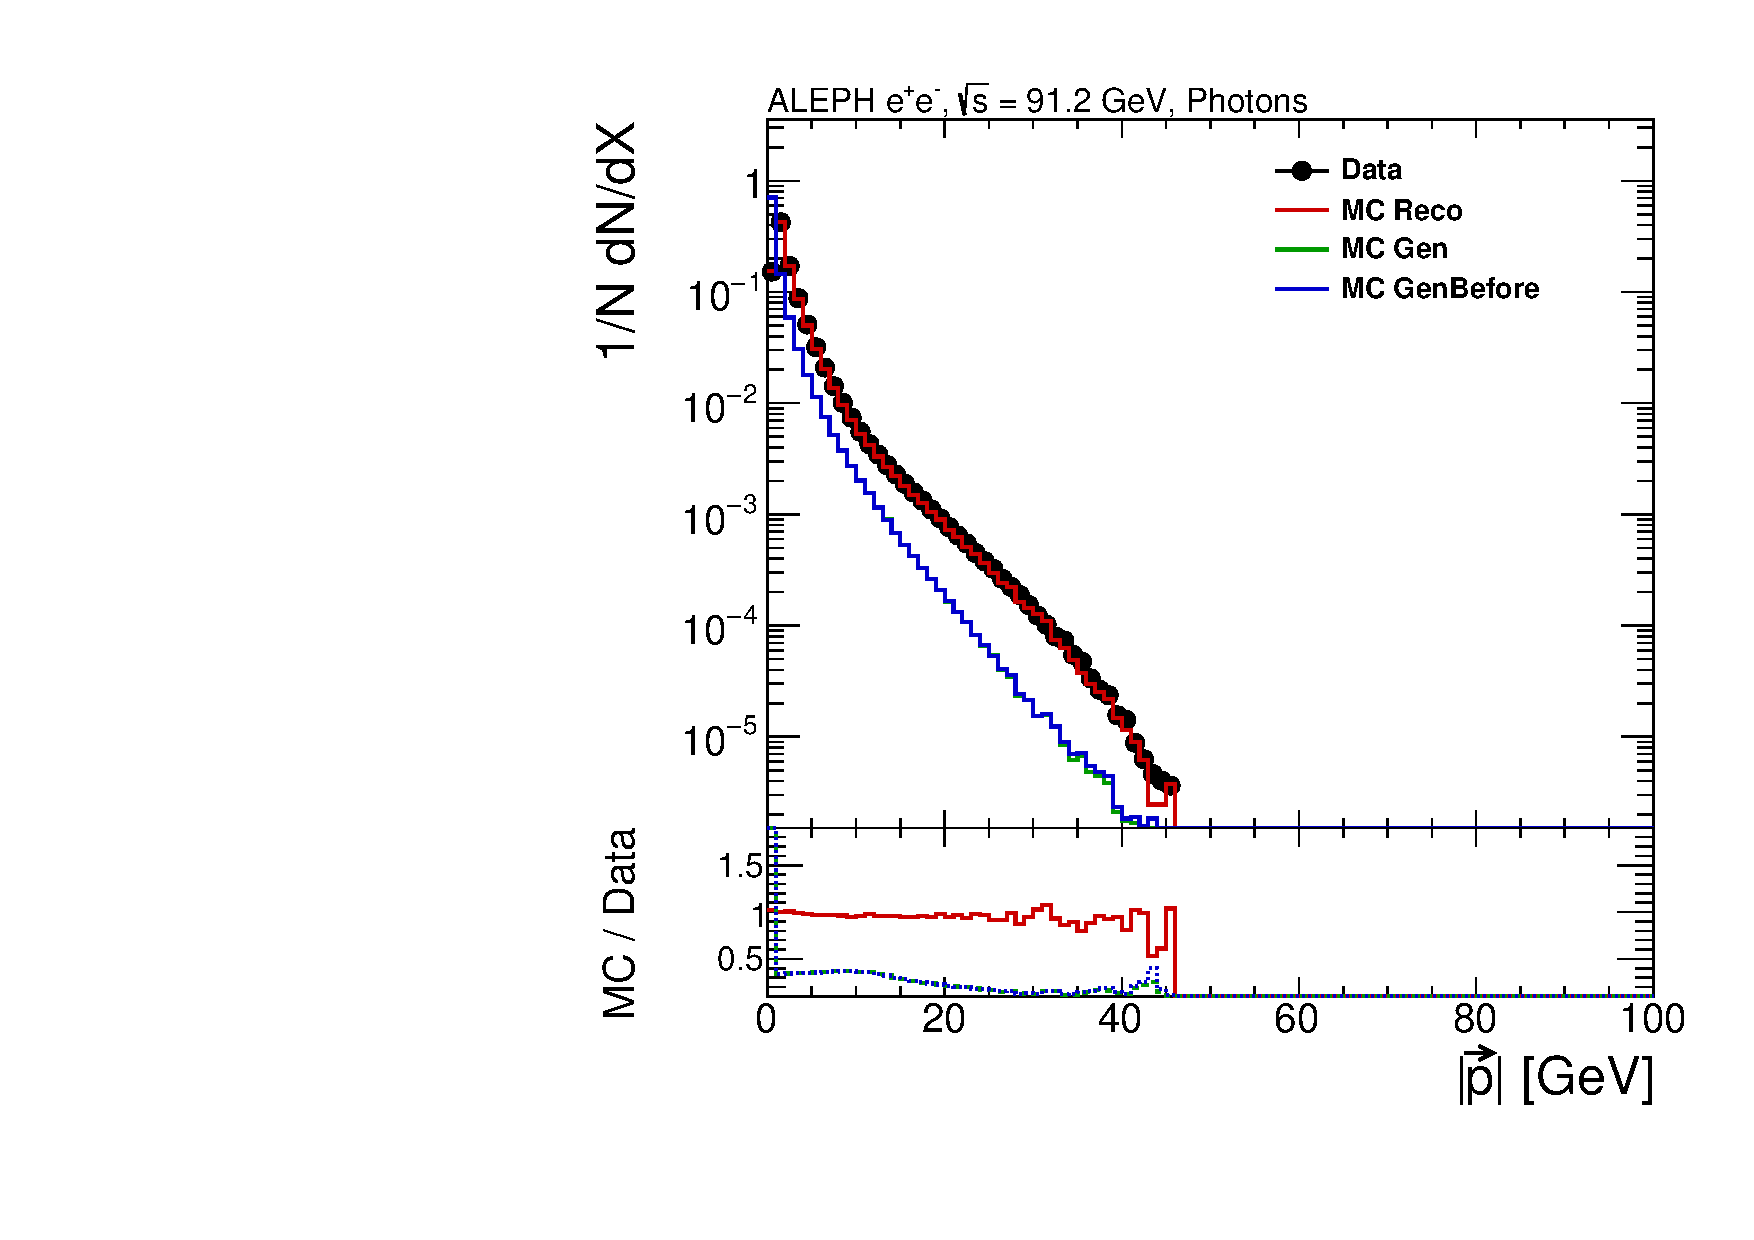
\includegraphics[width=0.325\textwidth]{../Studies/PreliminaryResult/2026-02-17_thrust_iter5/pwflag_kinematics/pwflag4_pmag.pdf}
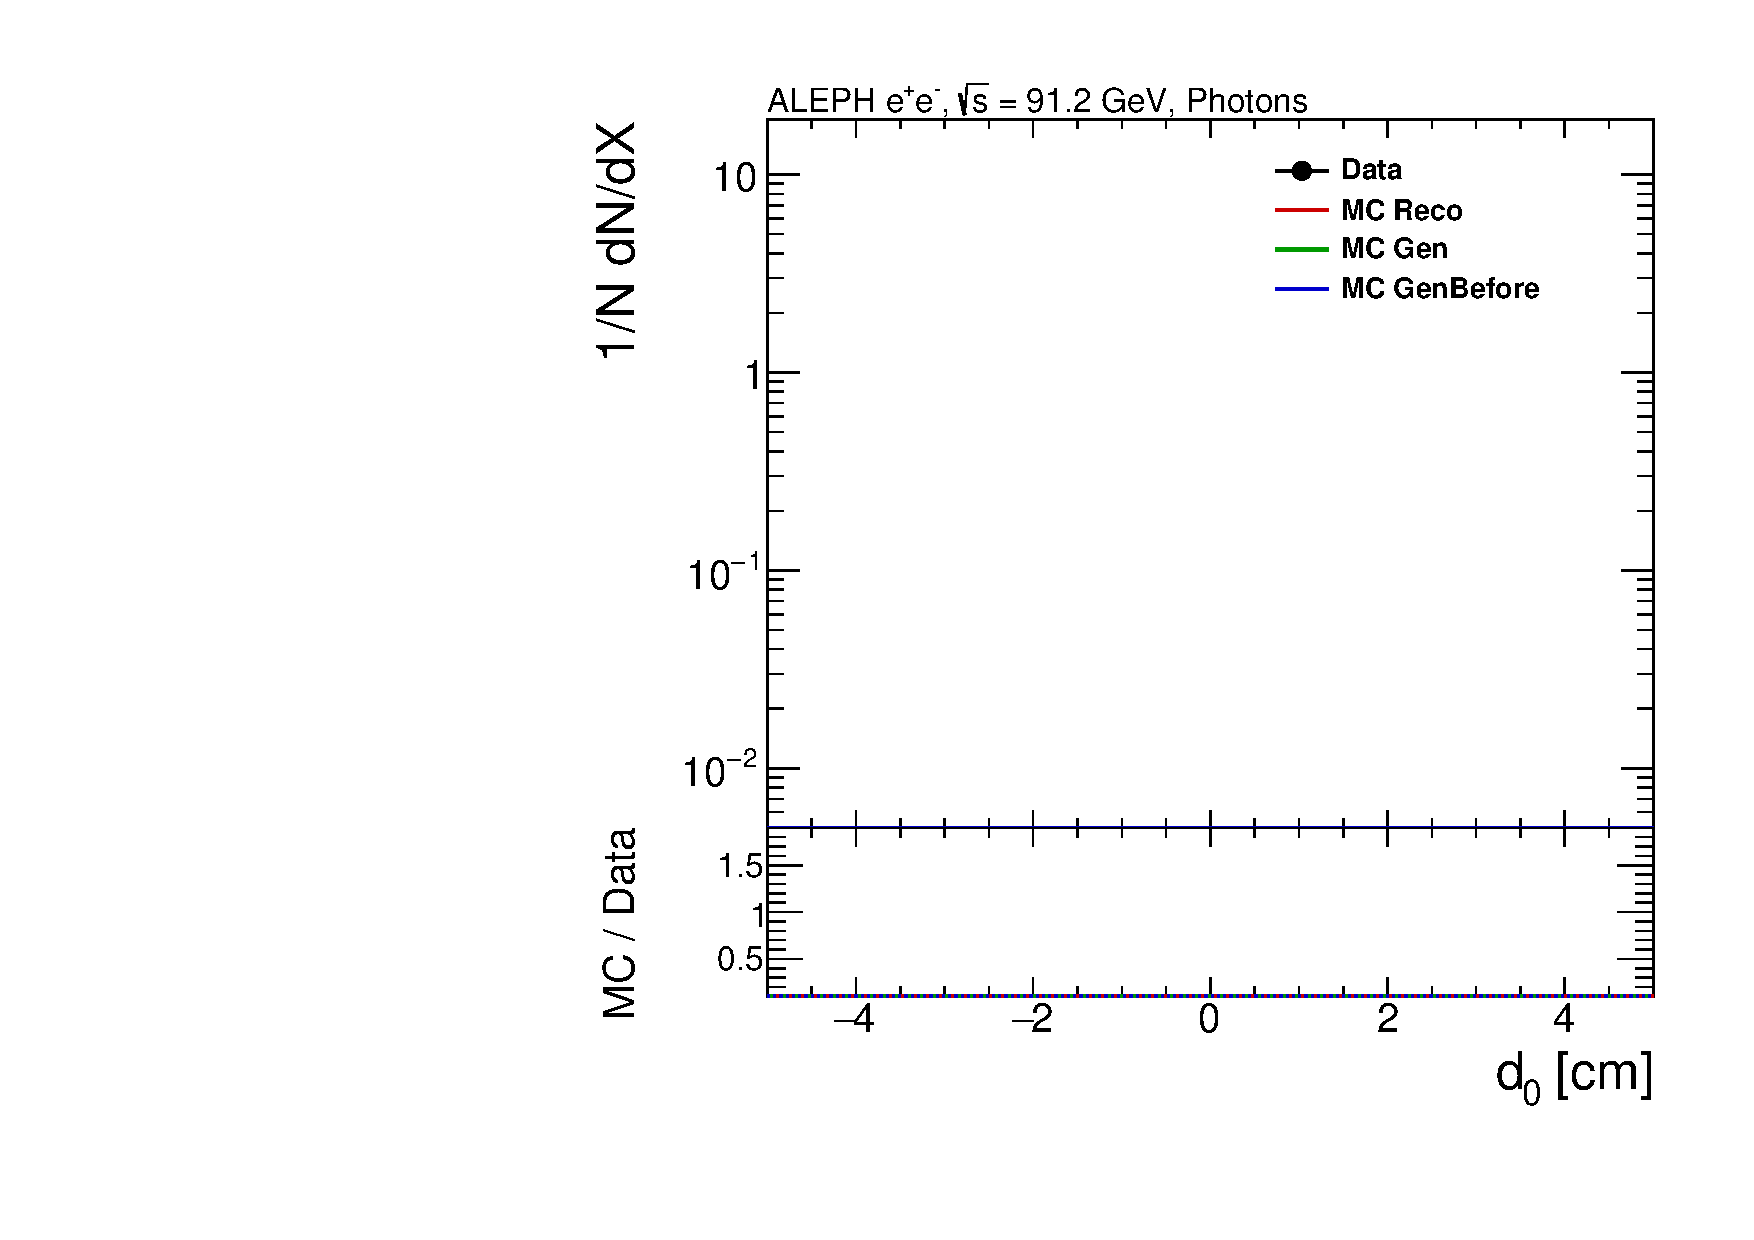
\includegraphics[width=0.325\textwidth]{../Studies/PreliminaryResult/2026-02-17_thrust_iter5/pwflag_kinematics/pwflag4_d0.pdf}
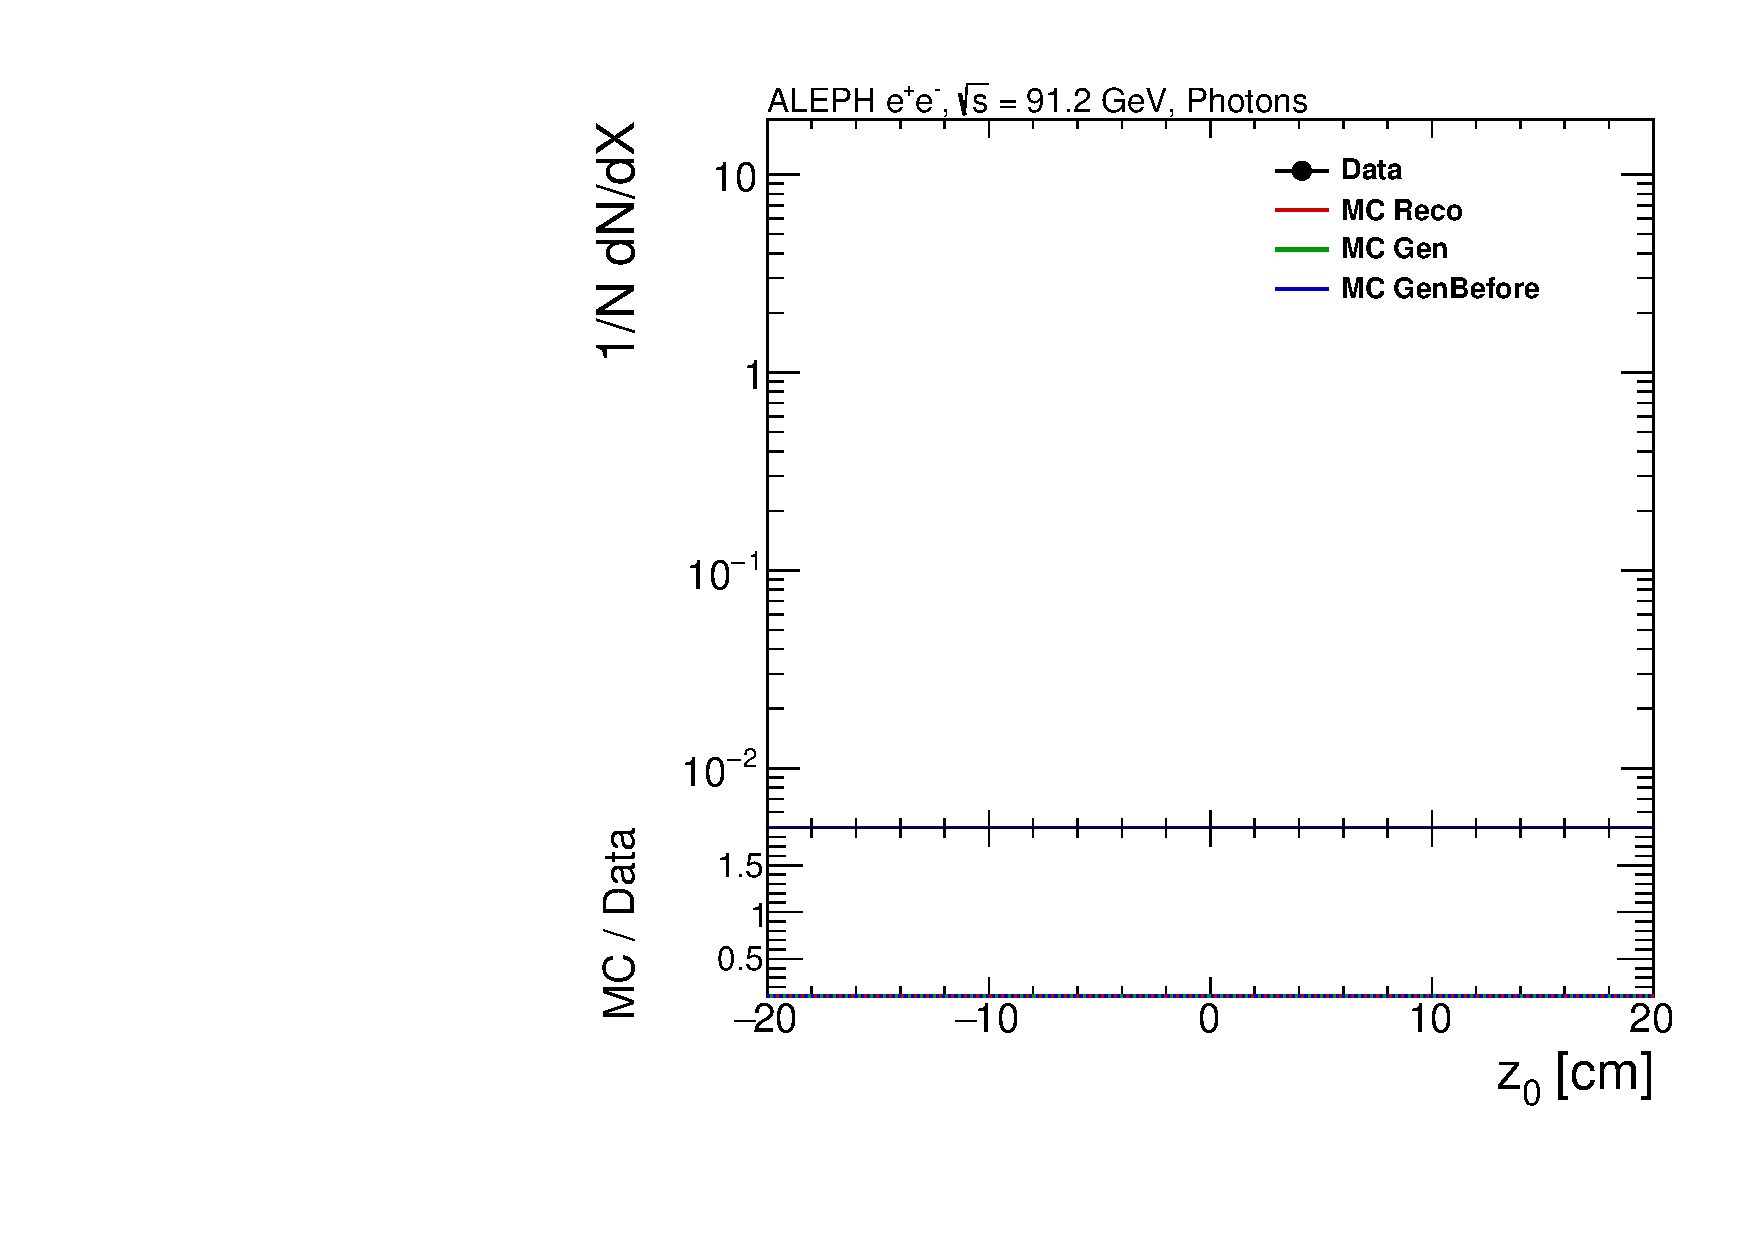
\includegraphics[width=0.325\textwidth]{../Studies/PreliminaryResult/2026-02-17_thrust_iter5/pwflag_kinematics/pwflag4_z0.pdf}
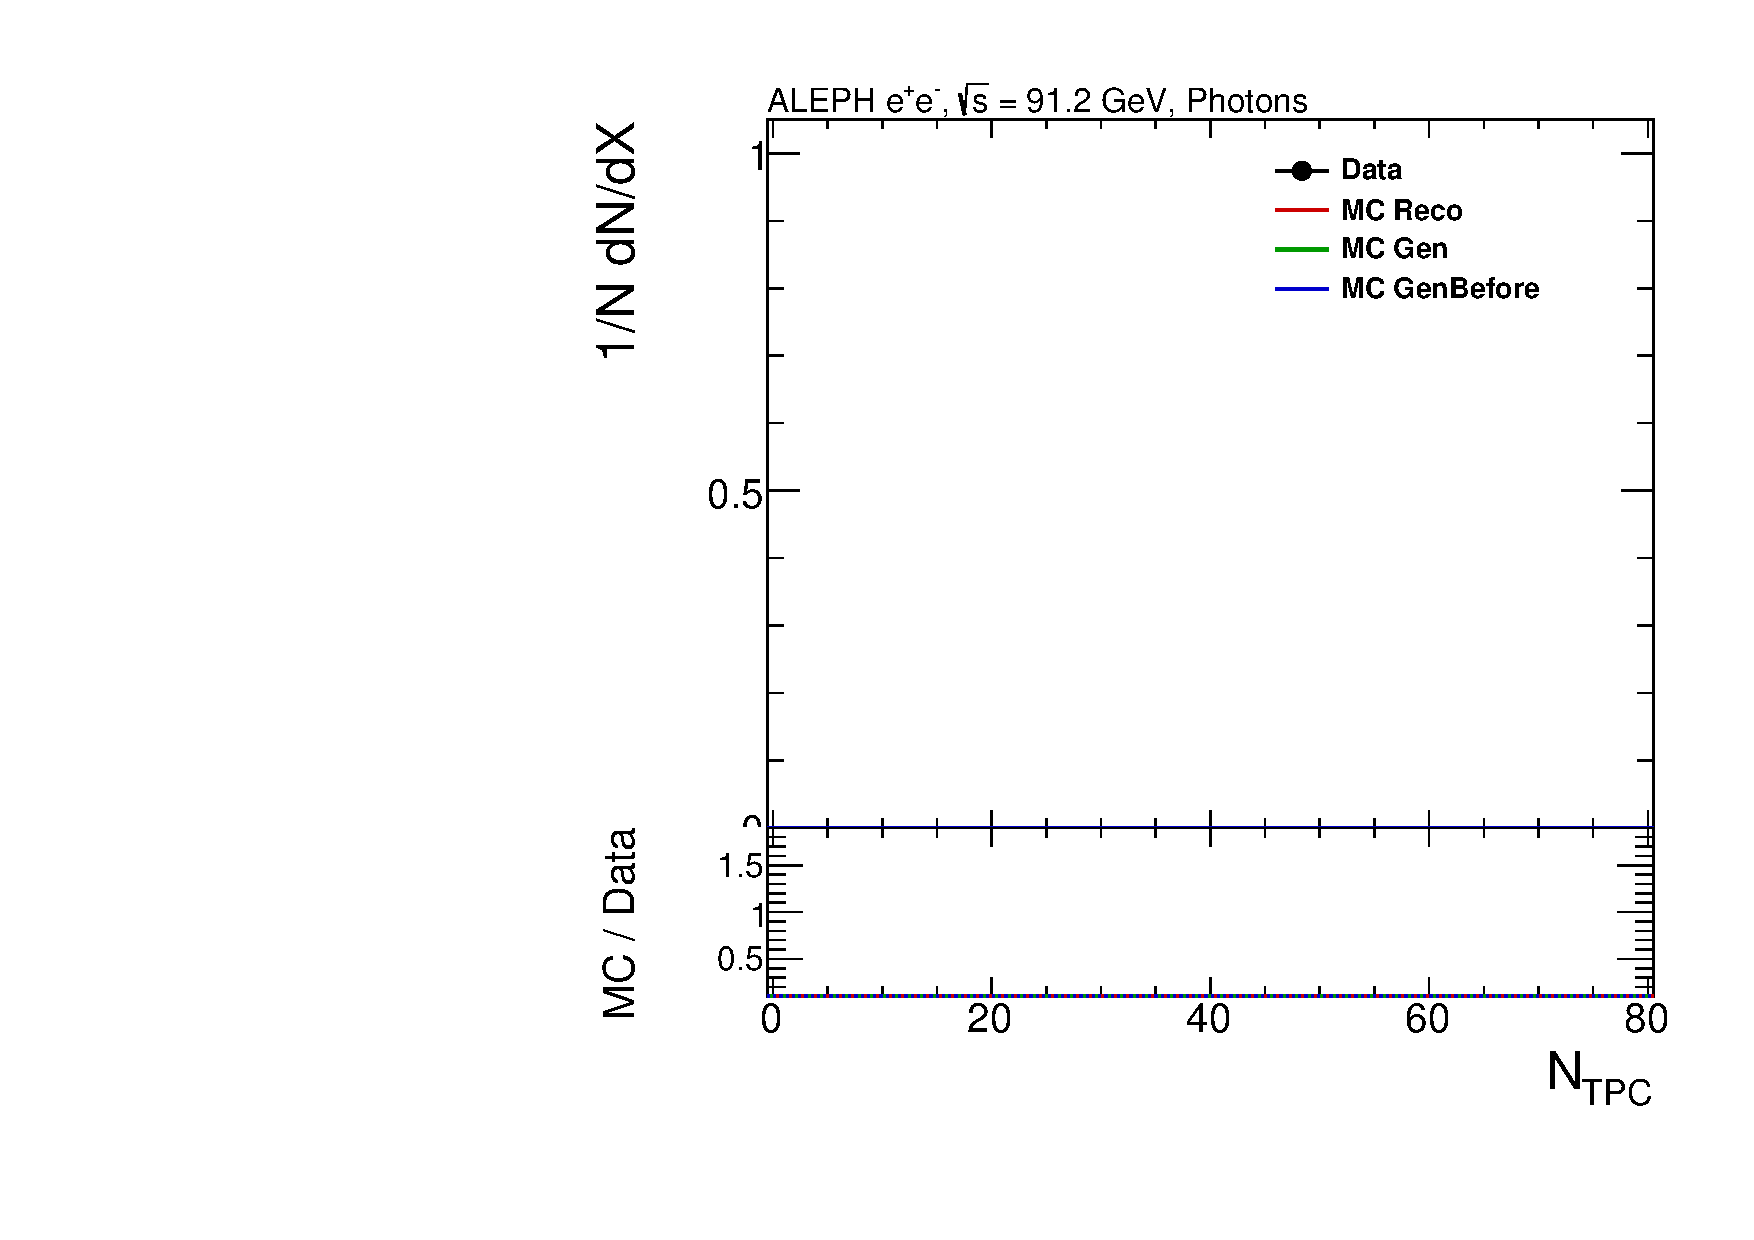
\includegraphics[width=0.325\textwidth]{../Studies/PreliminaryResult/2026-02-17_thrust_iter5/pwflag_kinematics/pwflag4_ntpc.pdf}
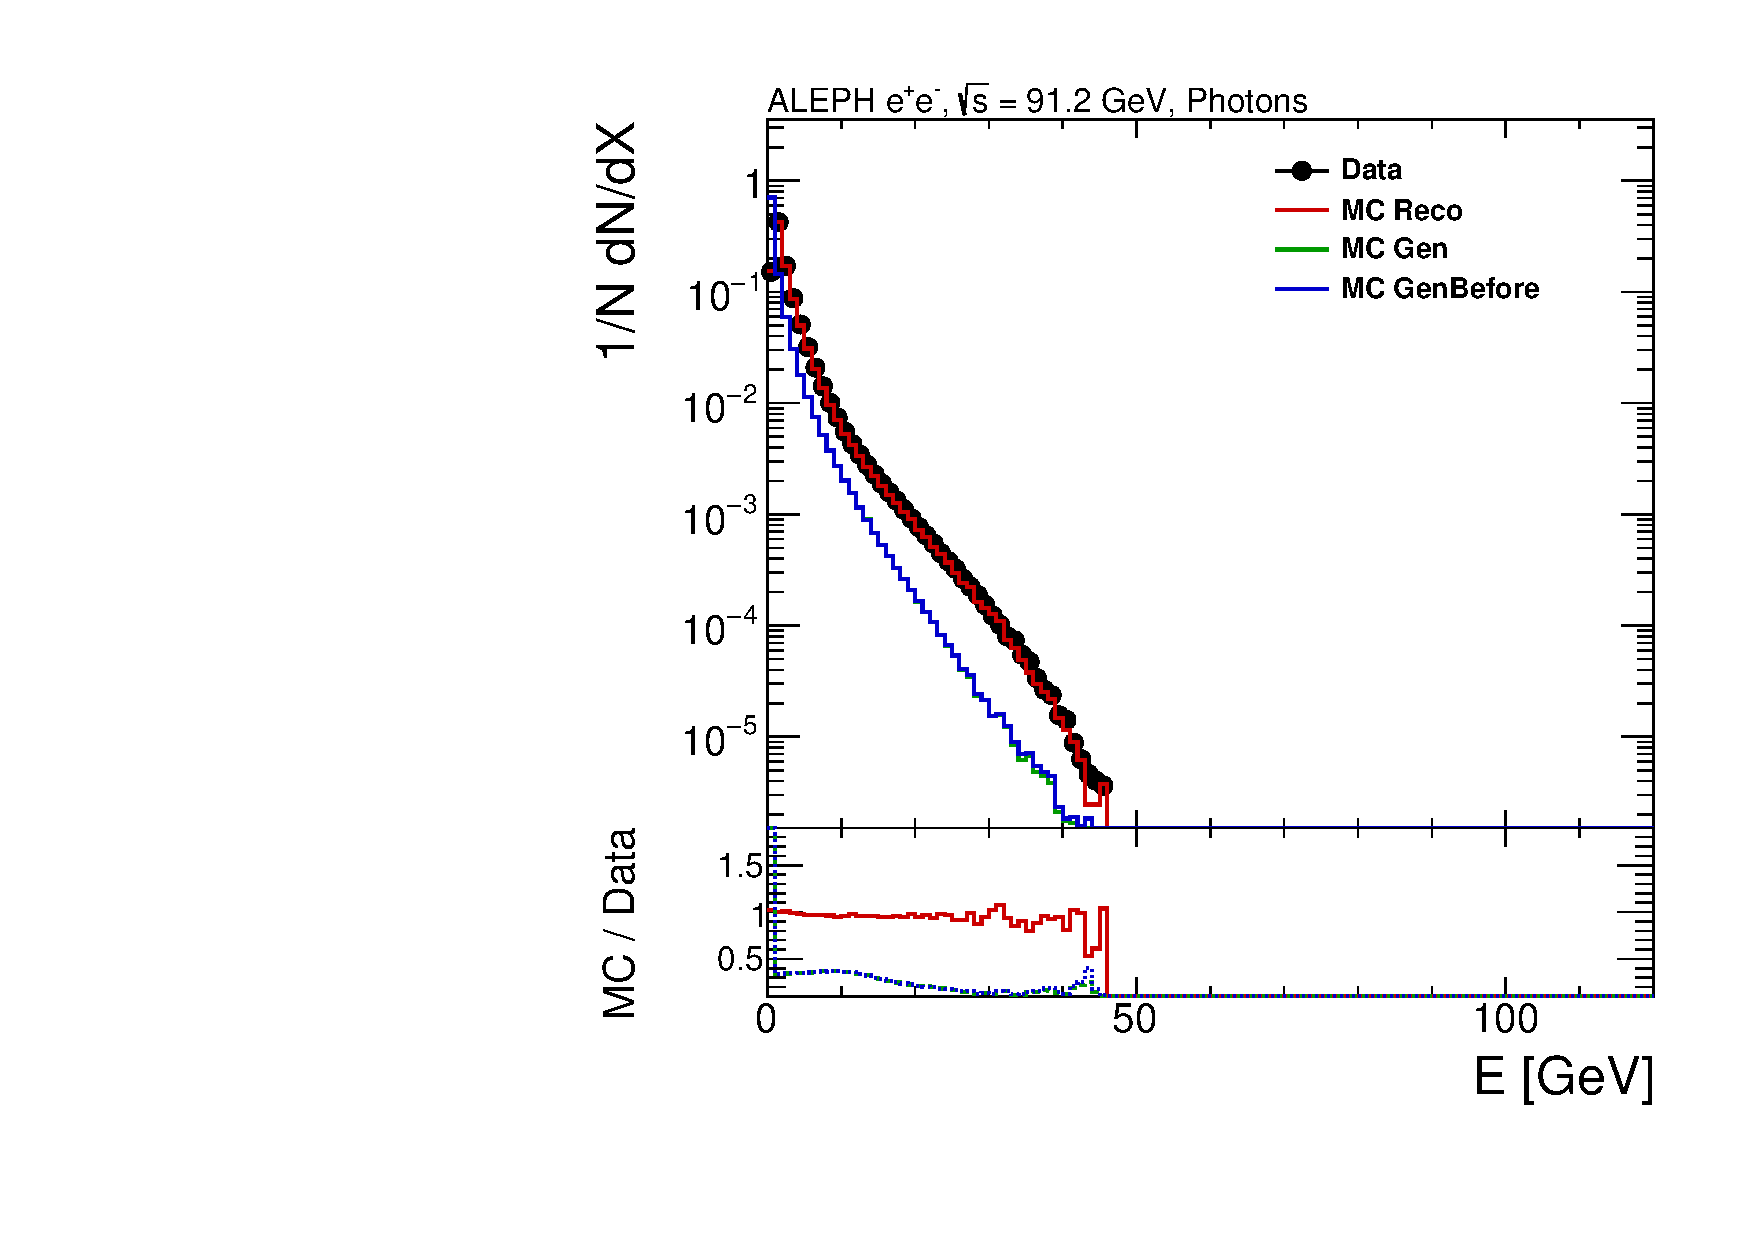
\includegraphics[width=0.325\textwidth]{../Studies/PreliminaryResult/2026-02-17_thrust_iter5/pwflag_kinematics/pwflag4_energy.pdf}
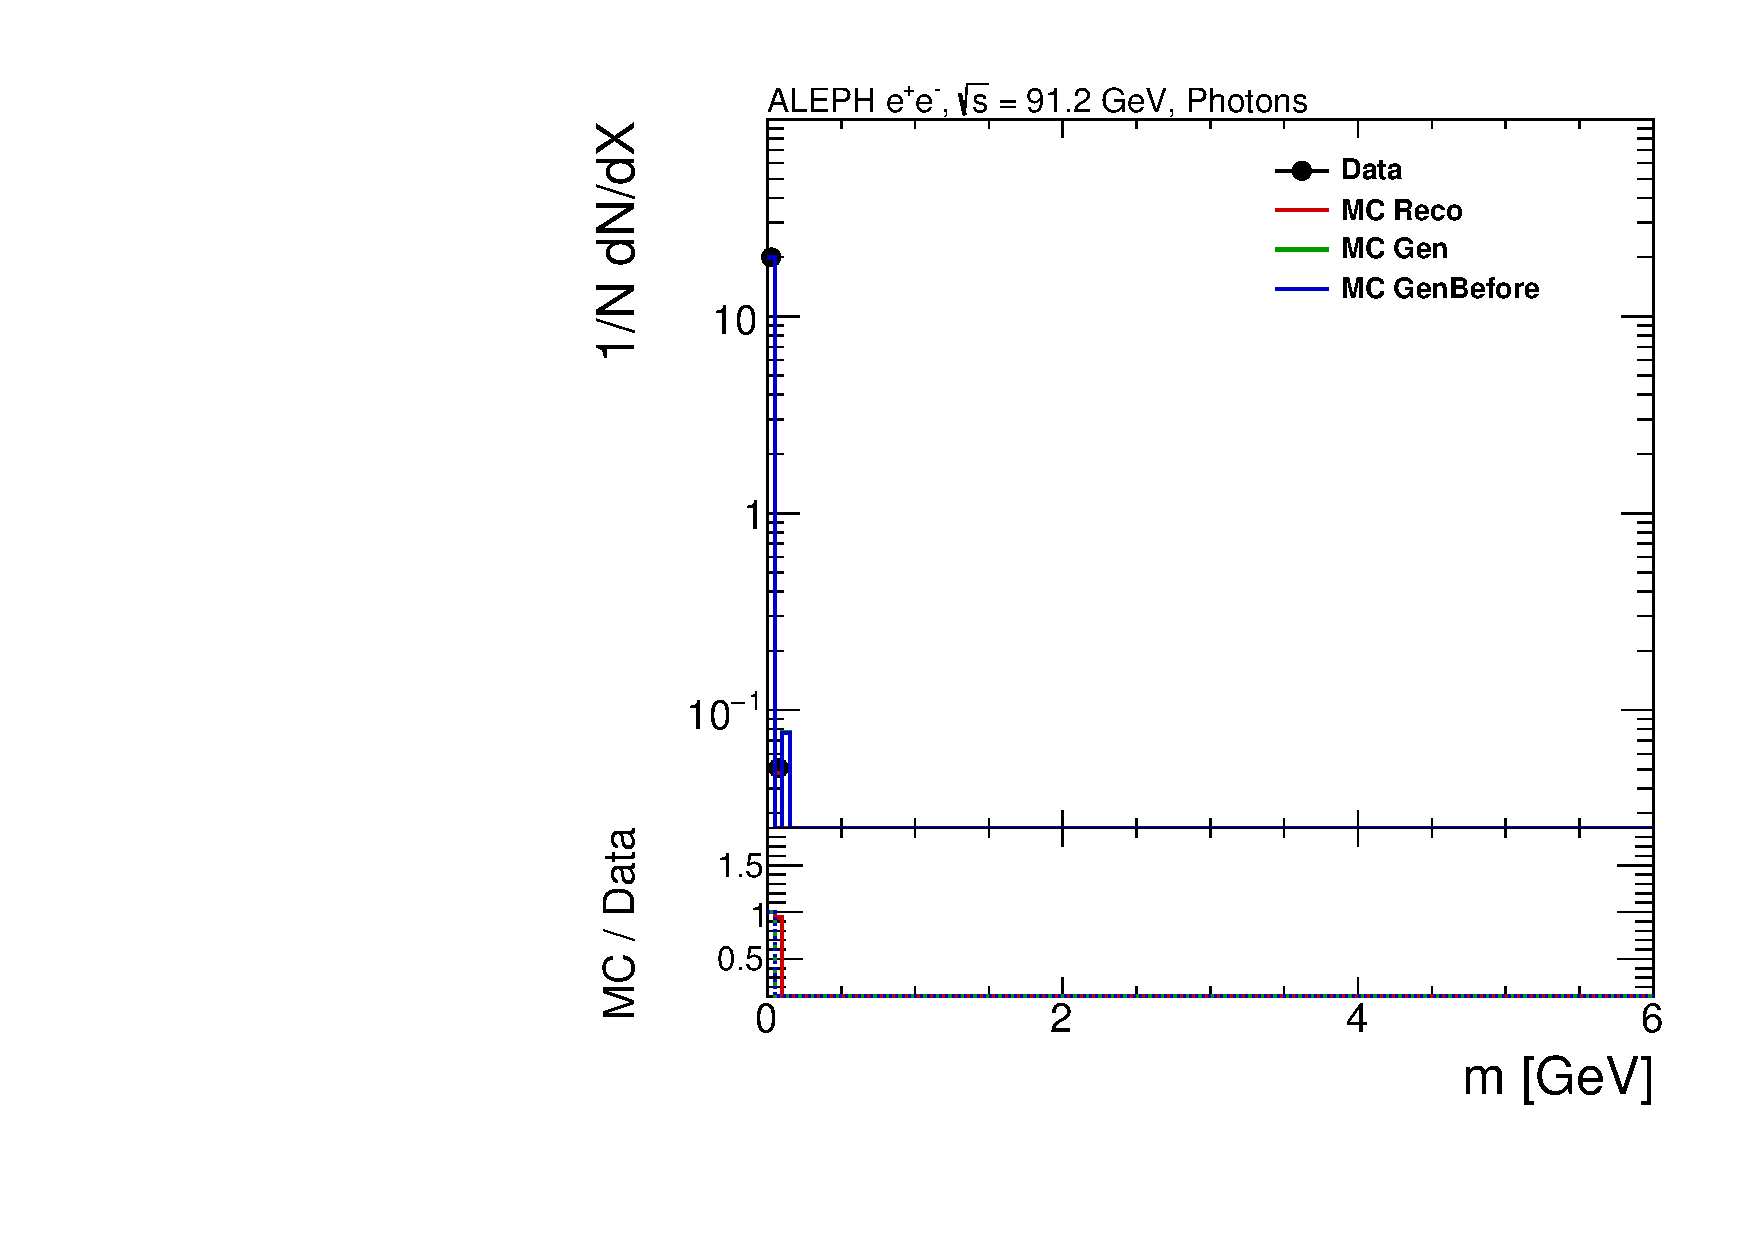
\includegraphics[width=0.325\textwidth]{../Studies/PreliminaryResult/2026-02-17_thrust_iter5/pwflag_kinematics/pwflag4_mass.pdf}
\caption{Complete \texttt{pwflag}=4 kinematic set.}
\label{fig:pwflag4_full}
\end{figure}

\noindent
Figure~\ref{fig:pwflag4_full} isolates photons, which probe neutral electromagnetic response and
its effect on event-shape normalization. The photon energy and angular spectra are especially
important because electromagnetic neutral energy contributes directly to visible event topology and
hemisphere energy balance. The observed data/MC consistency in the core region supports the
neutral-energy calibration assumptions used in the nominal unfolding and neutral-response
systematic variations.

\begin{figure}[t!]
\centering
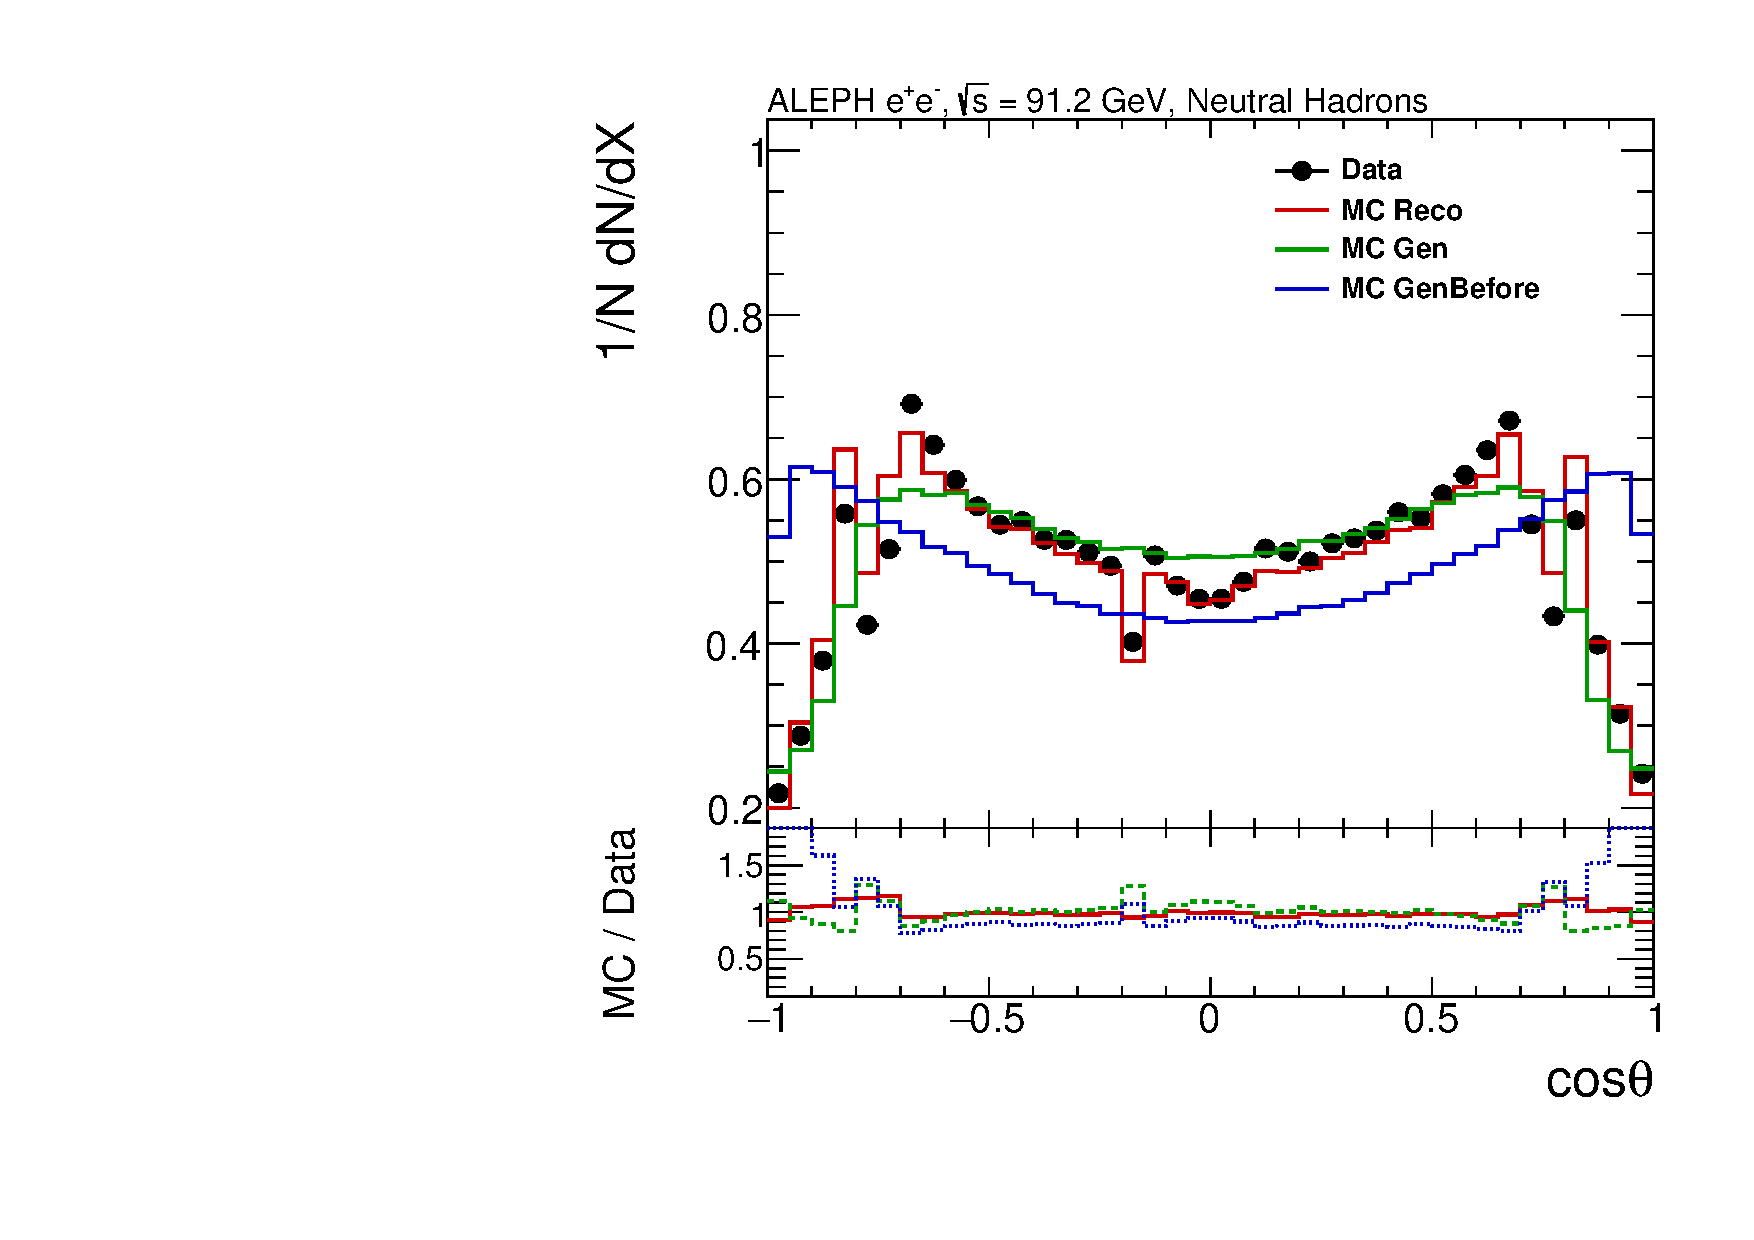
\includegraphics[width=0.325\textwidth]{../Studies/PreliminaryResult/2026-02-17_thrust_iter5/pwflag_kinematics/pwflag5_cosTheta.pdf}
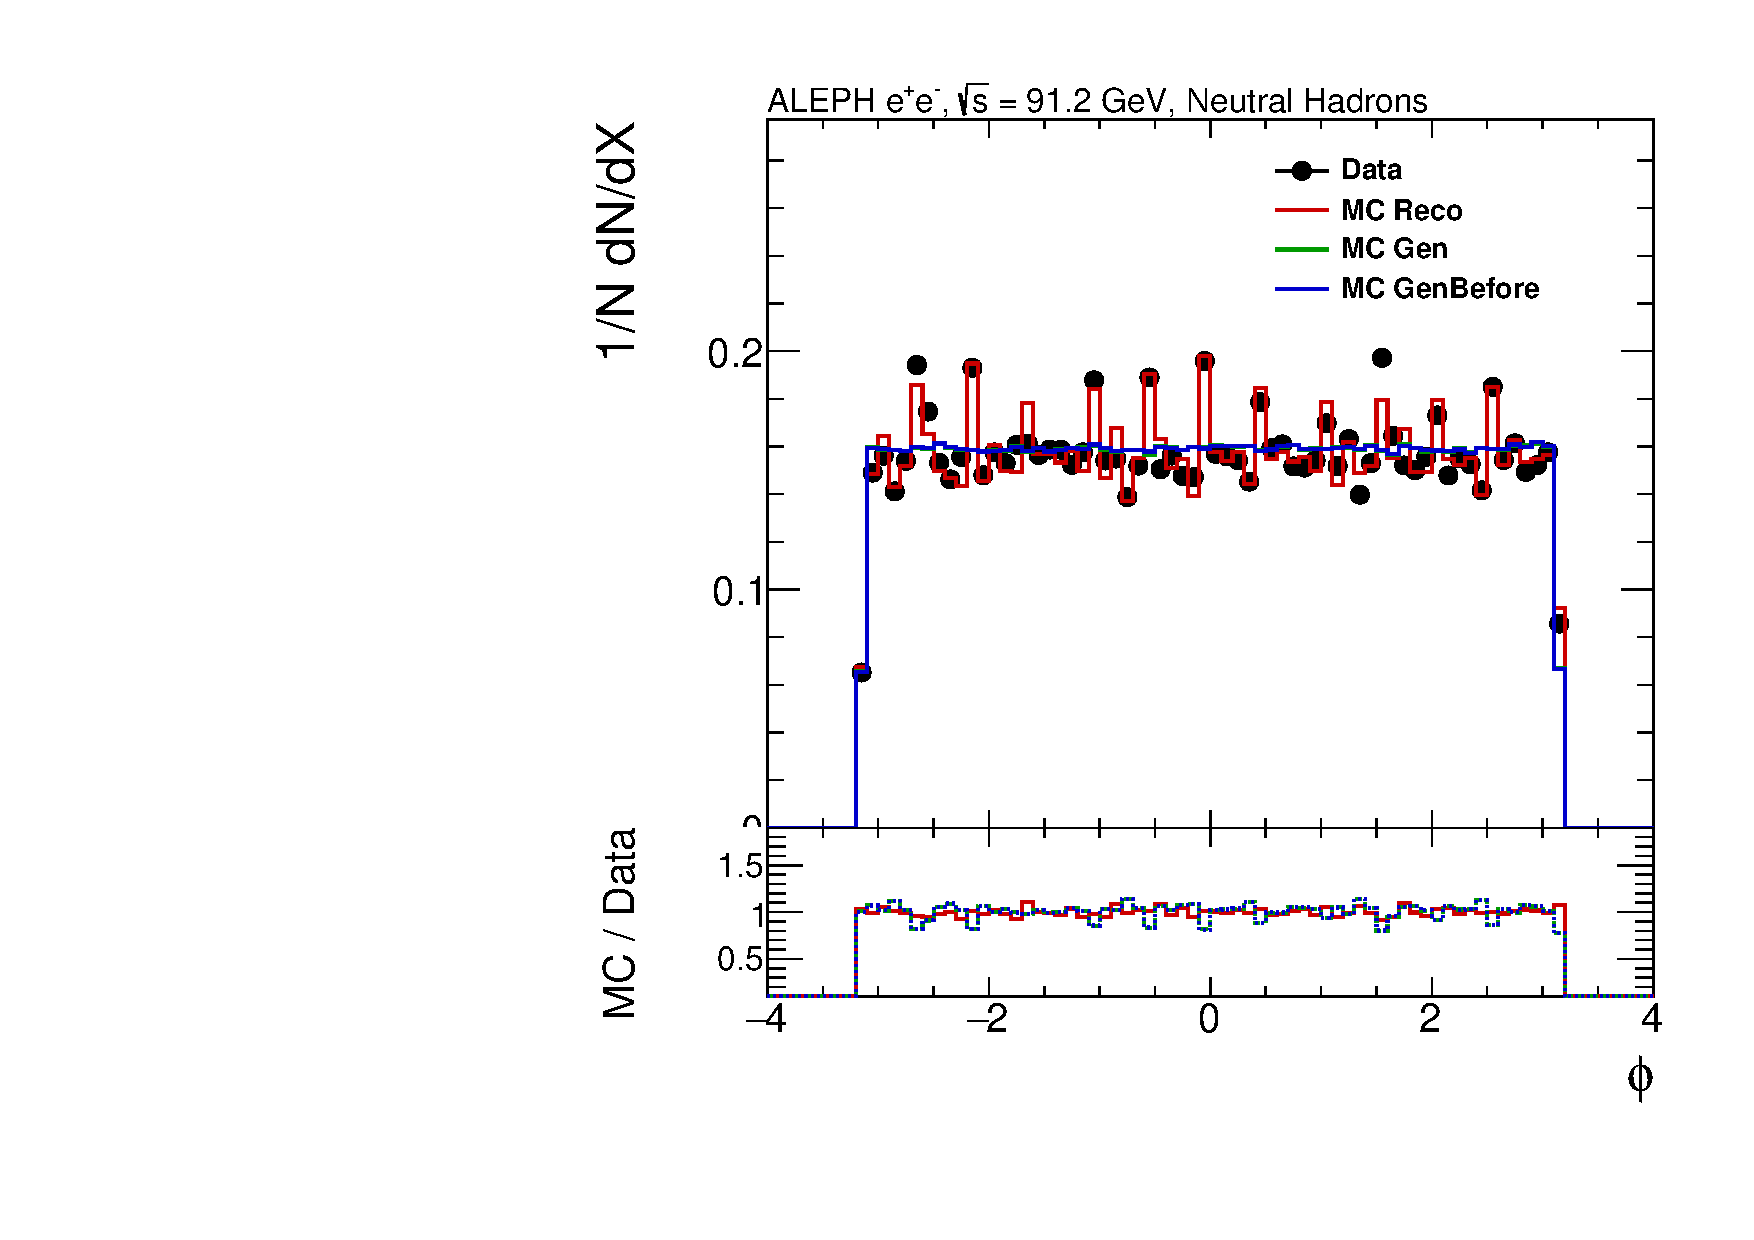
\includegraphics[width=0.325\textwidth]{../Studies/PreliminaryResult/2026-02-17_thrust_iter5/pwflag_kinematics/pwflag5_phi.pdf}
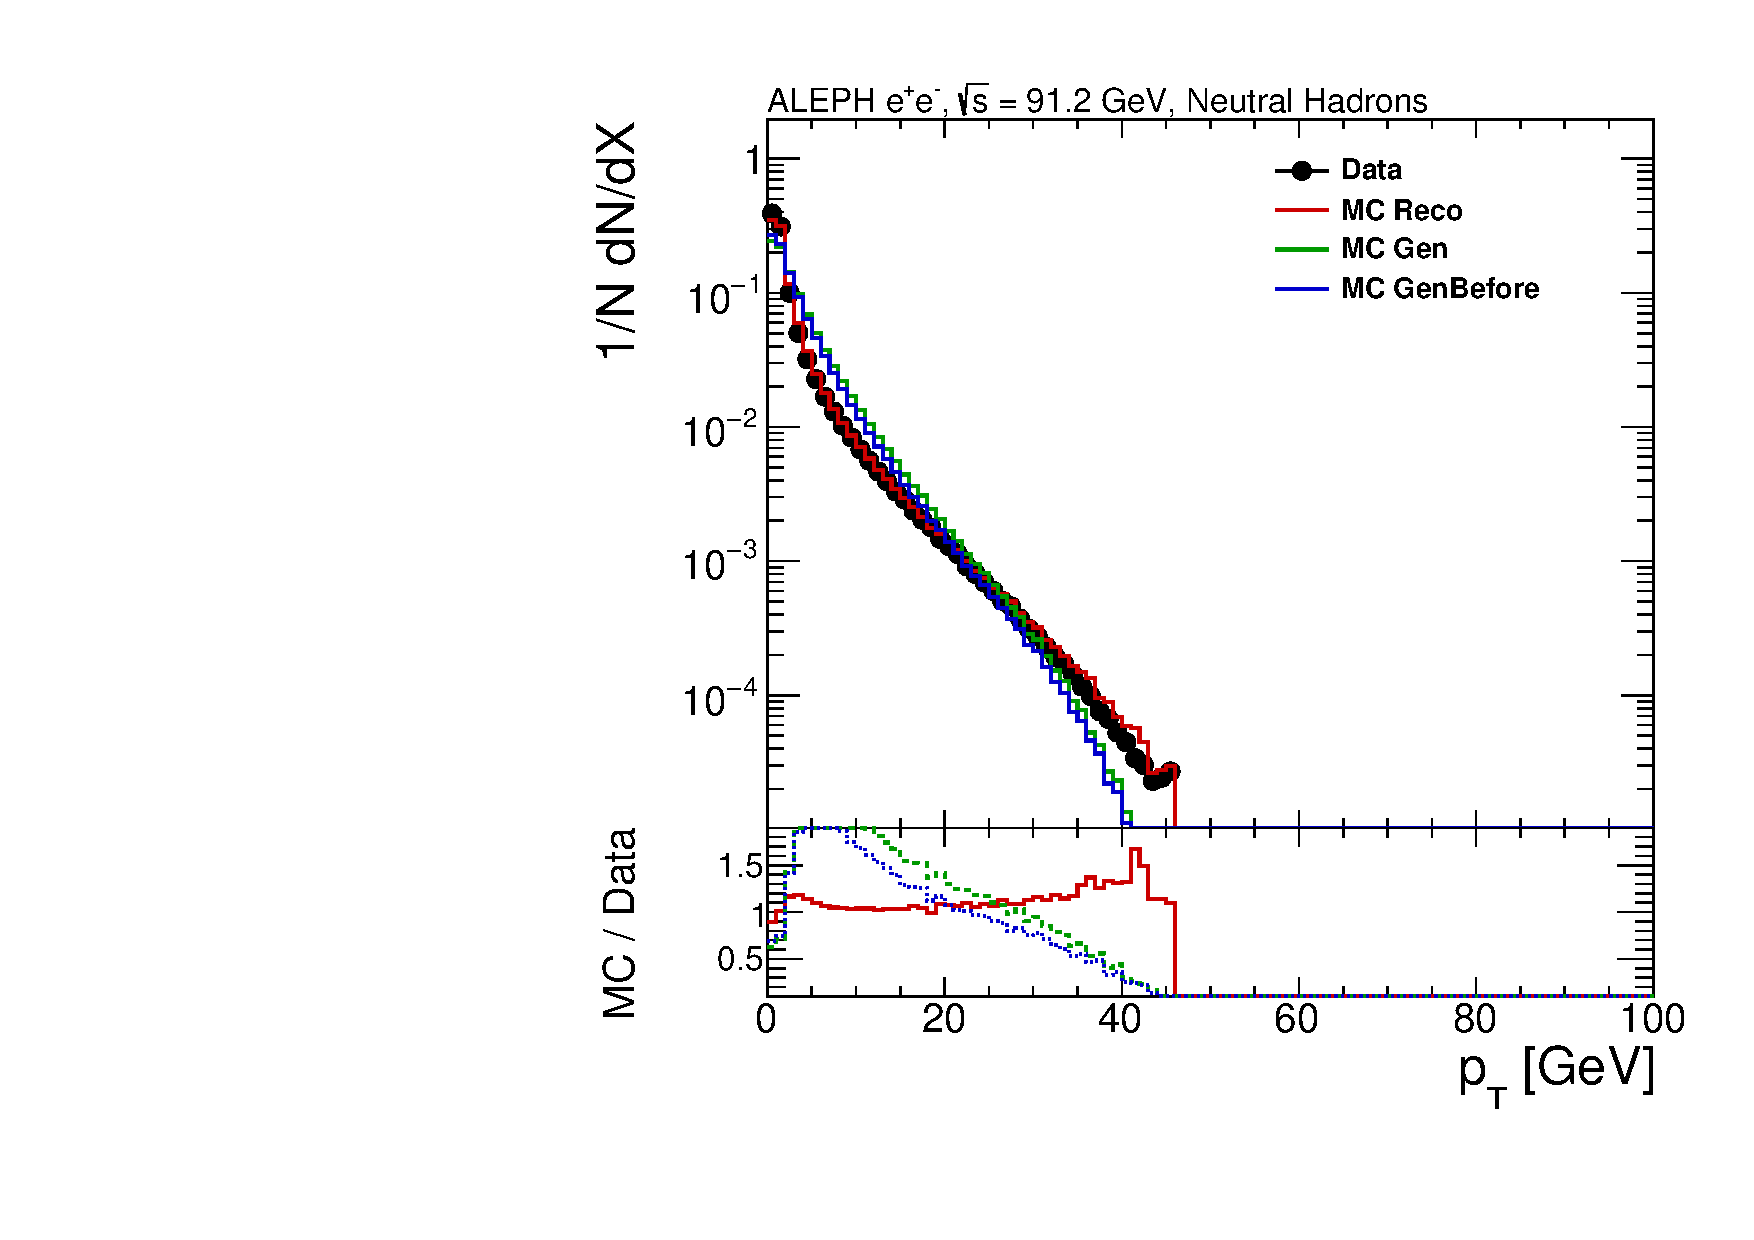
\includegraphics[width=0.325\textwidth]{../Studies/PreliminaryResult/2026-02-17_thrust_iter5/pwflag_kinematics/pwflag5_pt.pdf}
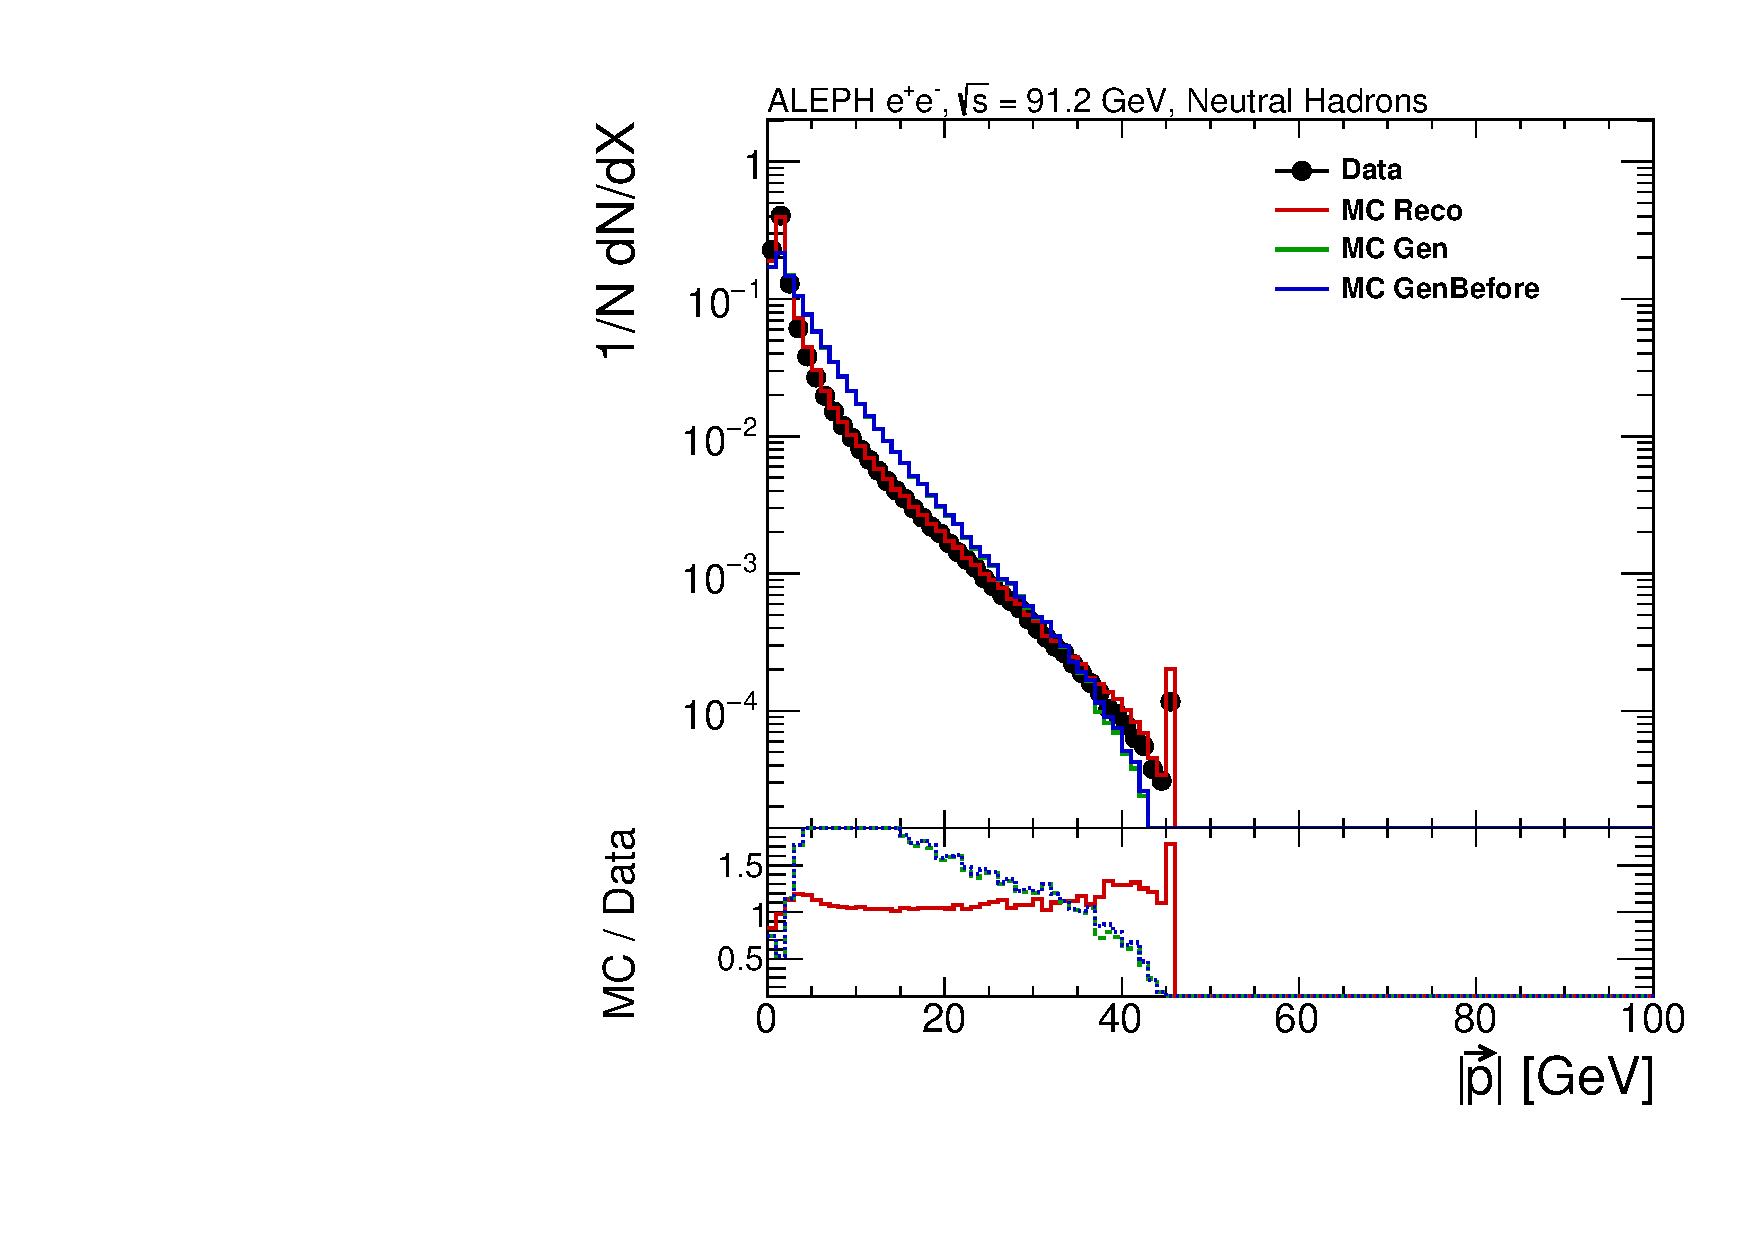
\includegraphics[width=0.325\textwidth]{../Studies/PreliminaryResult/2026-02-17_thrust_iter5/pwflag_kinematics/pwflag5_pmag.pdf}
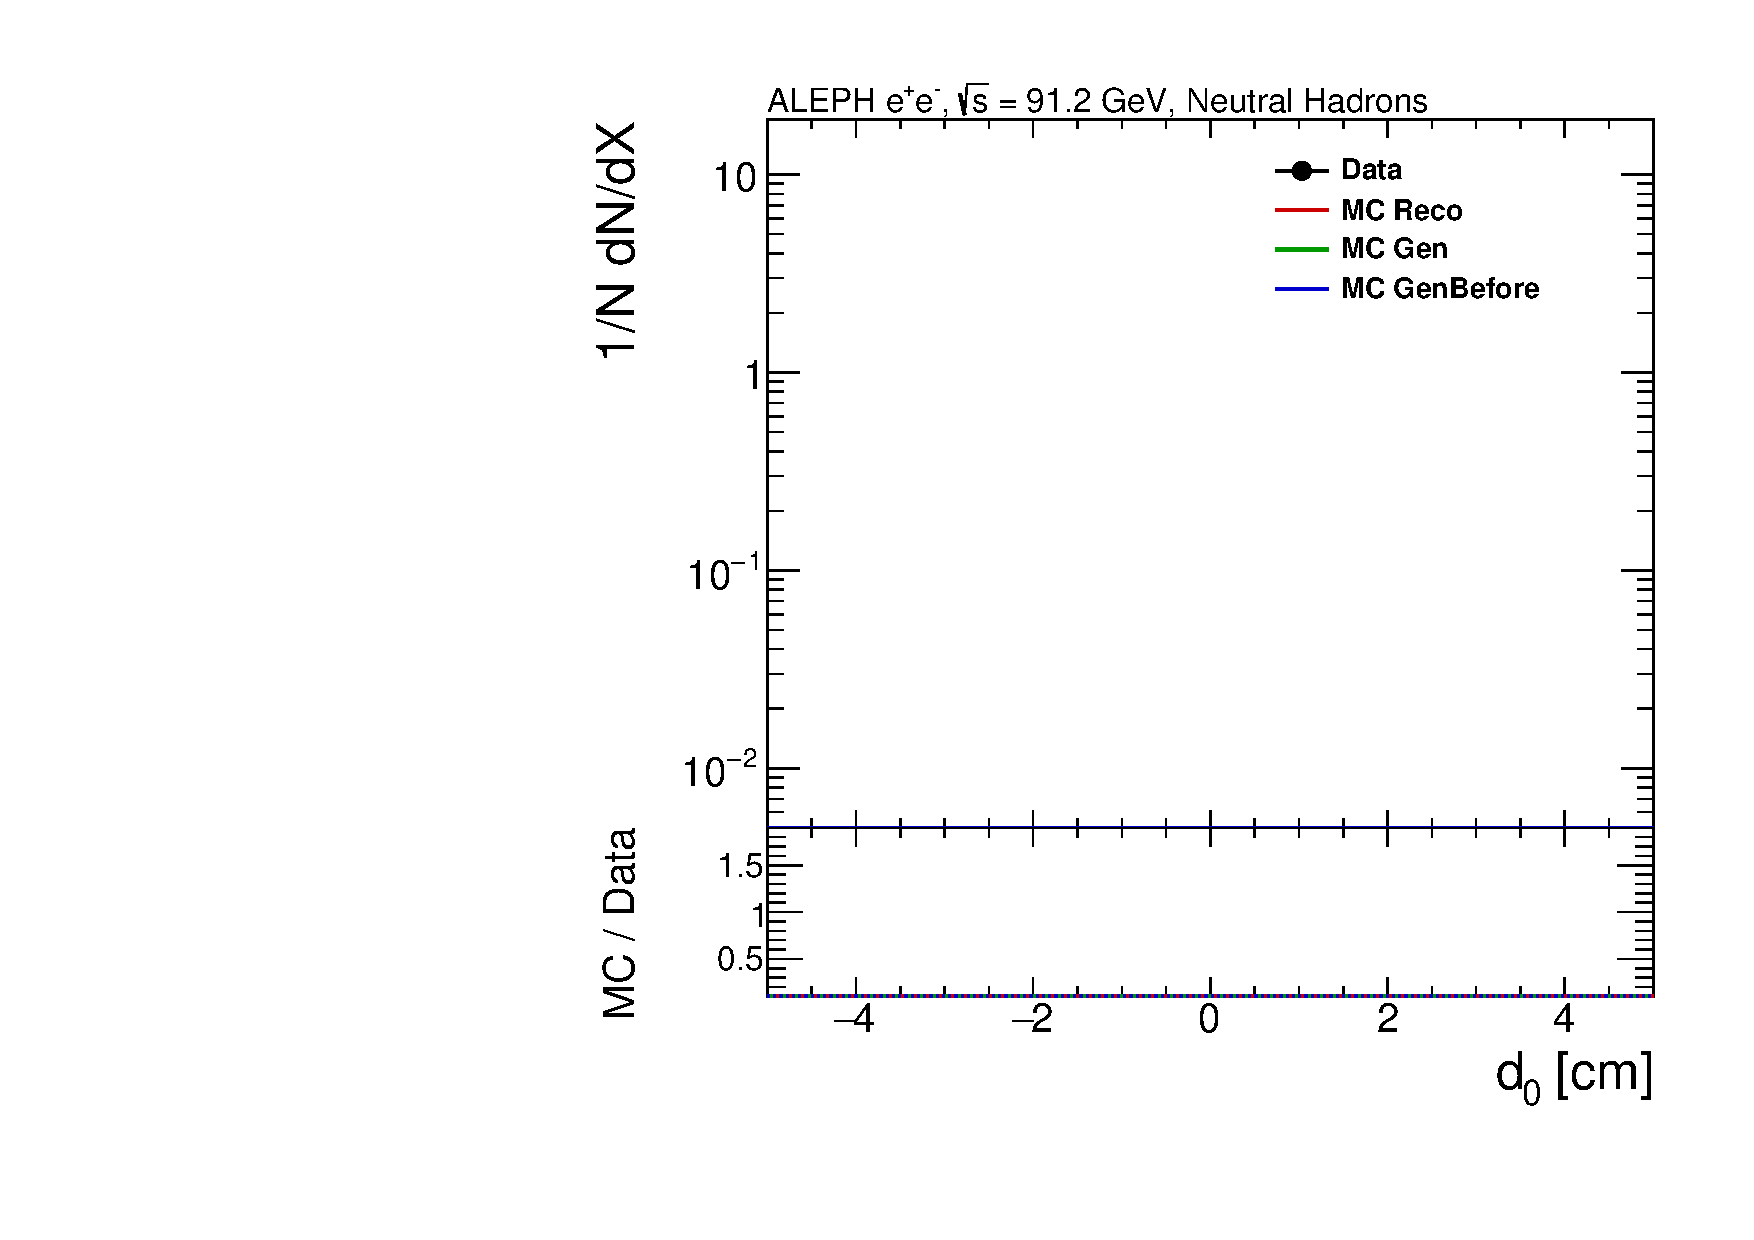
\includegraphics[width=0.325\textwidth]{../Studies/PreliminaryResult/2026-02-17_thrust_iter5/pwflag_kinematics/pwflag5_d0.pdf}
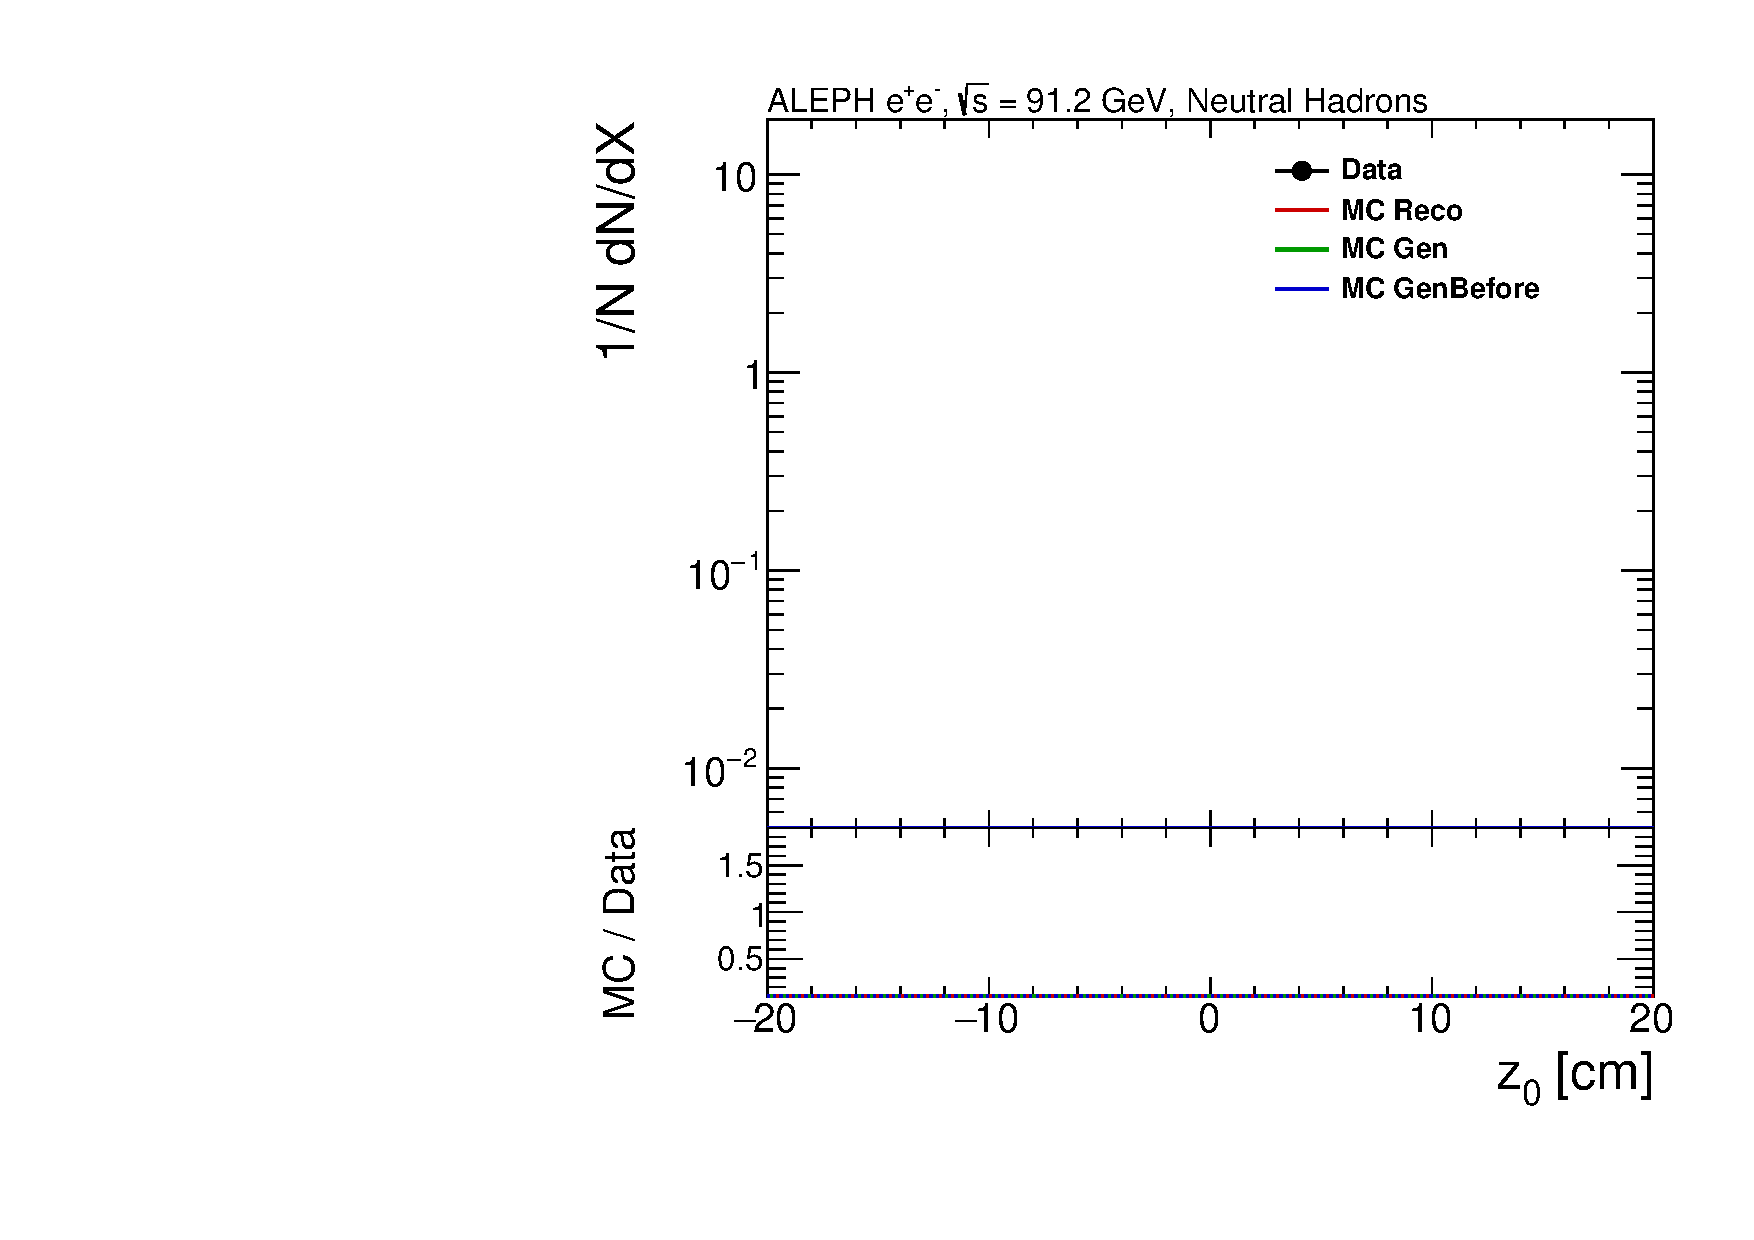
\includegraphics[width=0.325\textwidth]{../Studies/PreliminaryResult/2026-02-17_thrust_iter5/pwflag_kinematics/pwflag5_z0.pdf}
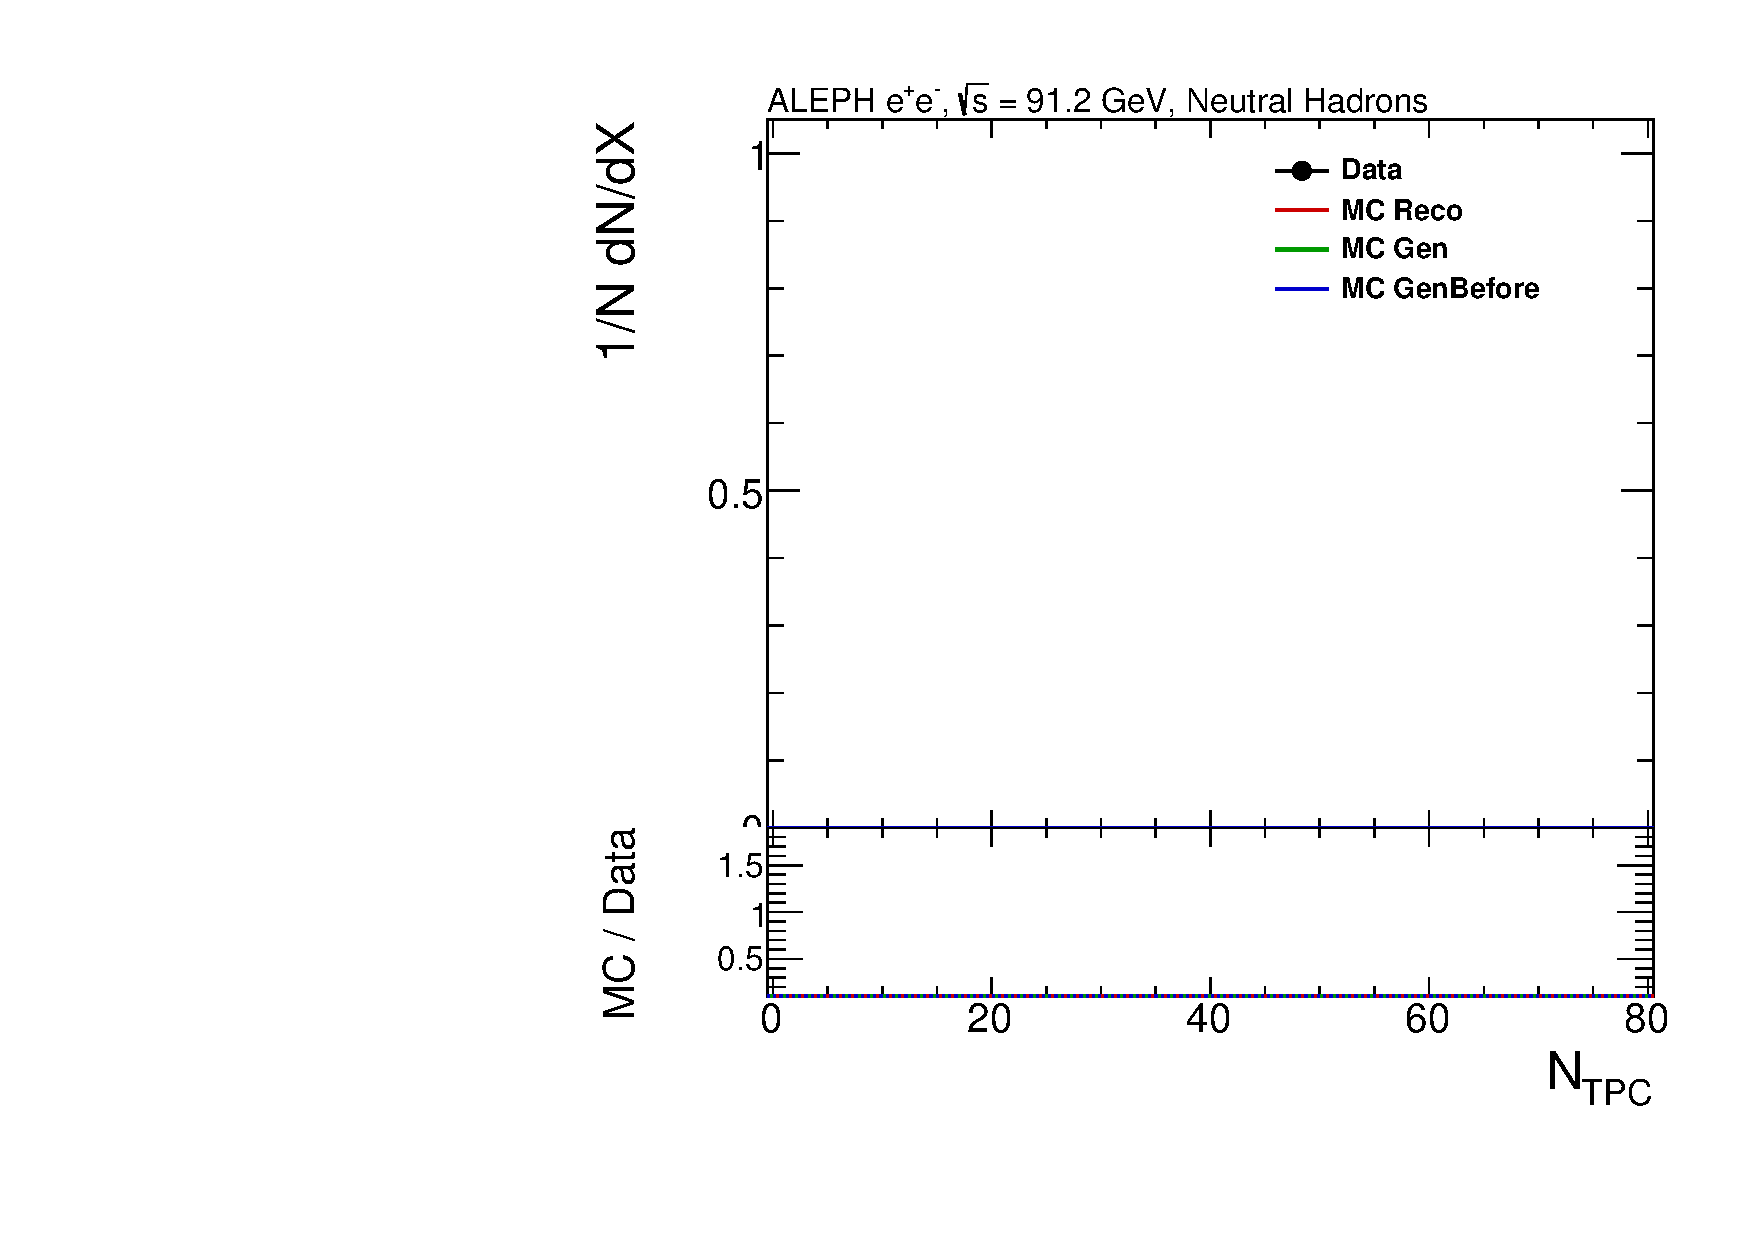
\includegraphics[width=0.325\textwidth]{../Studies/PreliminaryResult/2026-02-17_thrust_iter5/pwflag_kinematics/pwflag5_ntpc.pdf}
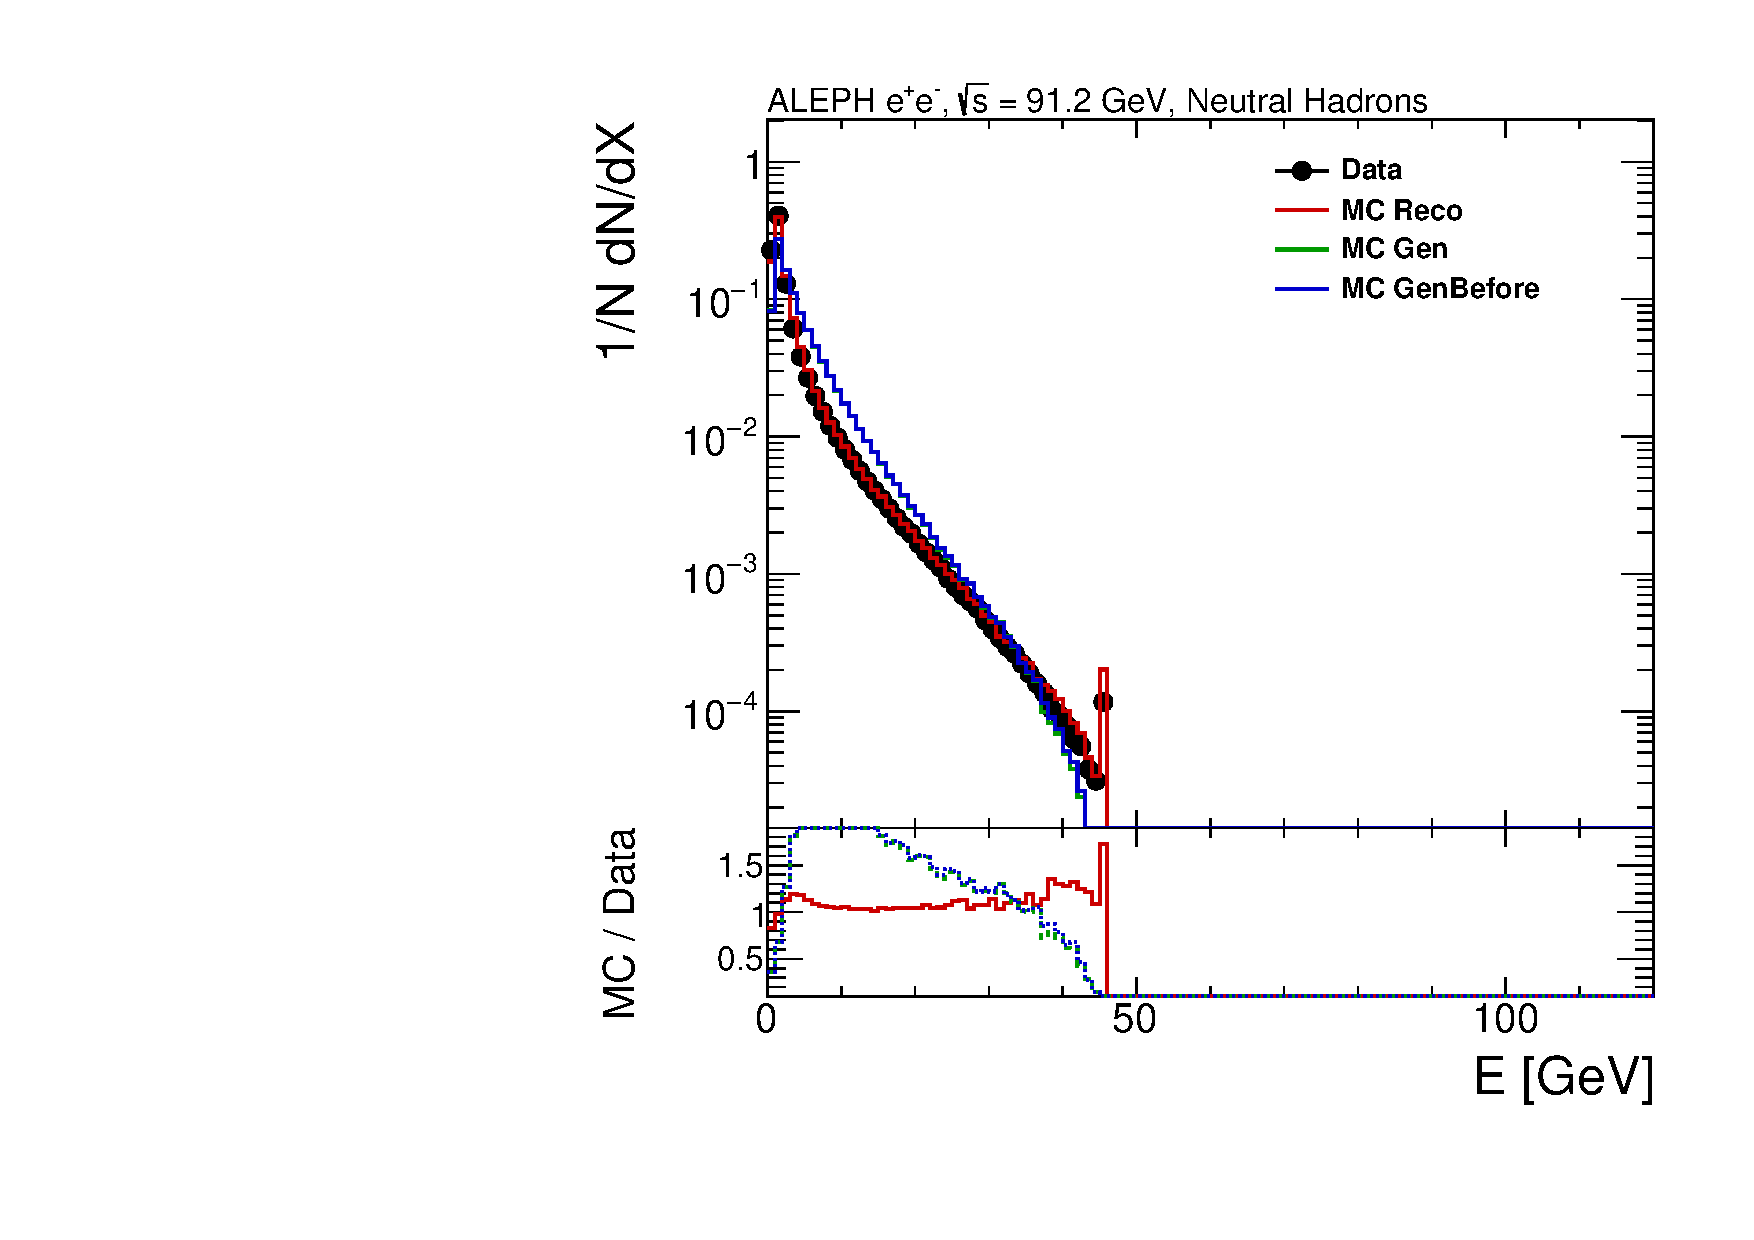
\includegraphics[width=0.325\textwidth]{../Studies/PreliminaryResult/2026-02-17_thrust_iter5/pwflag_kinematics/pwflag5_energy.pdf}
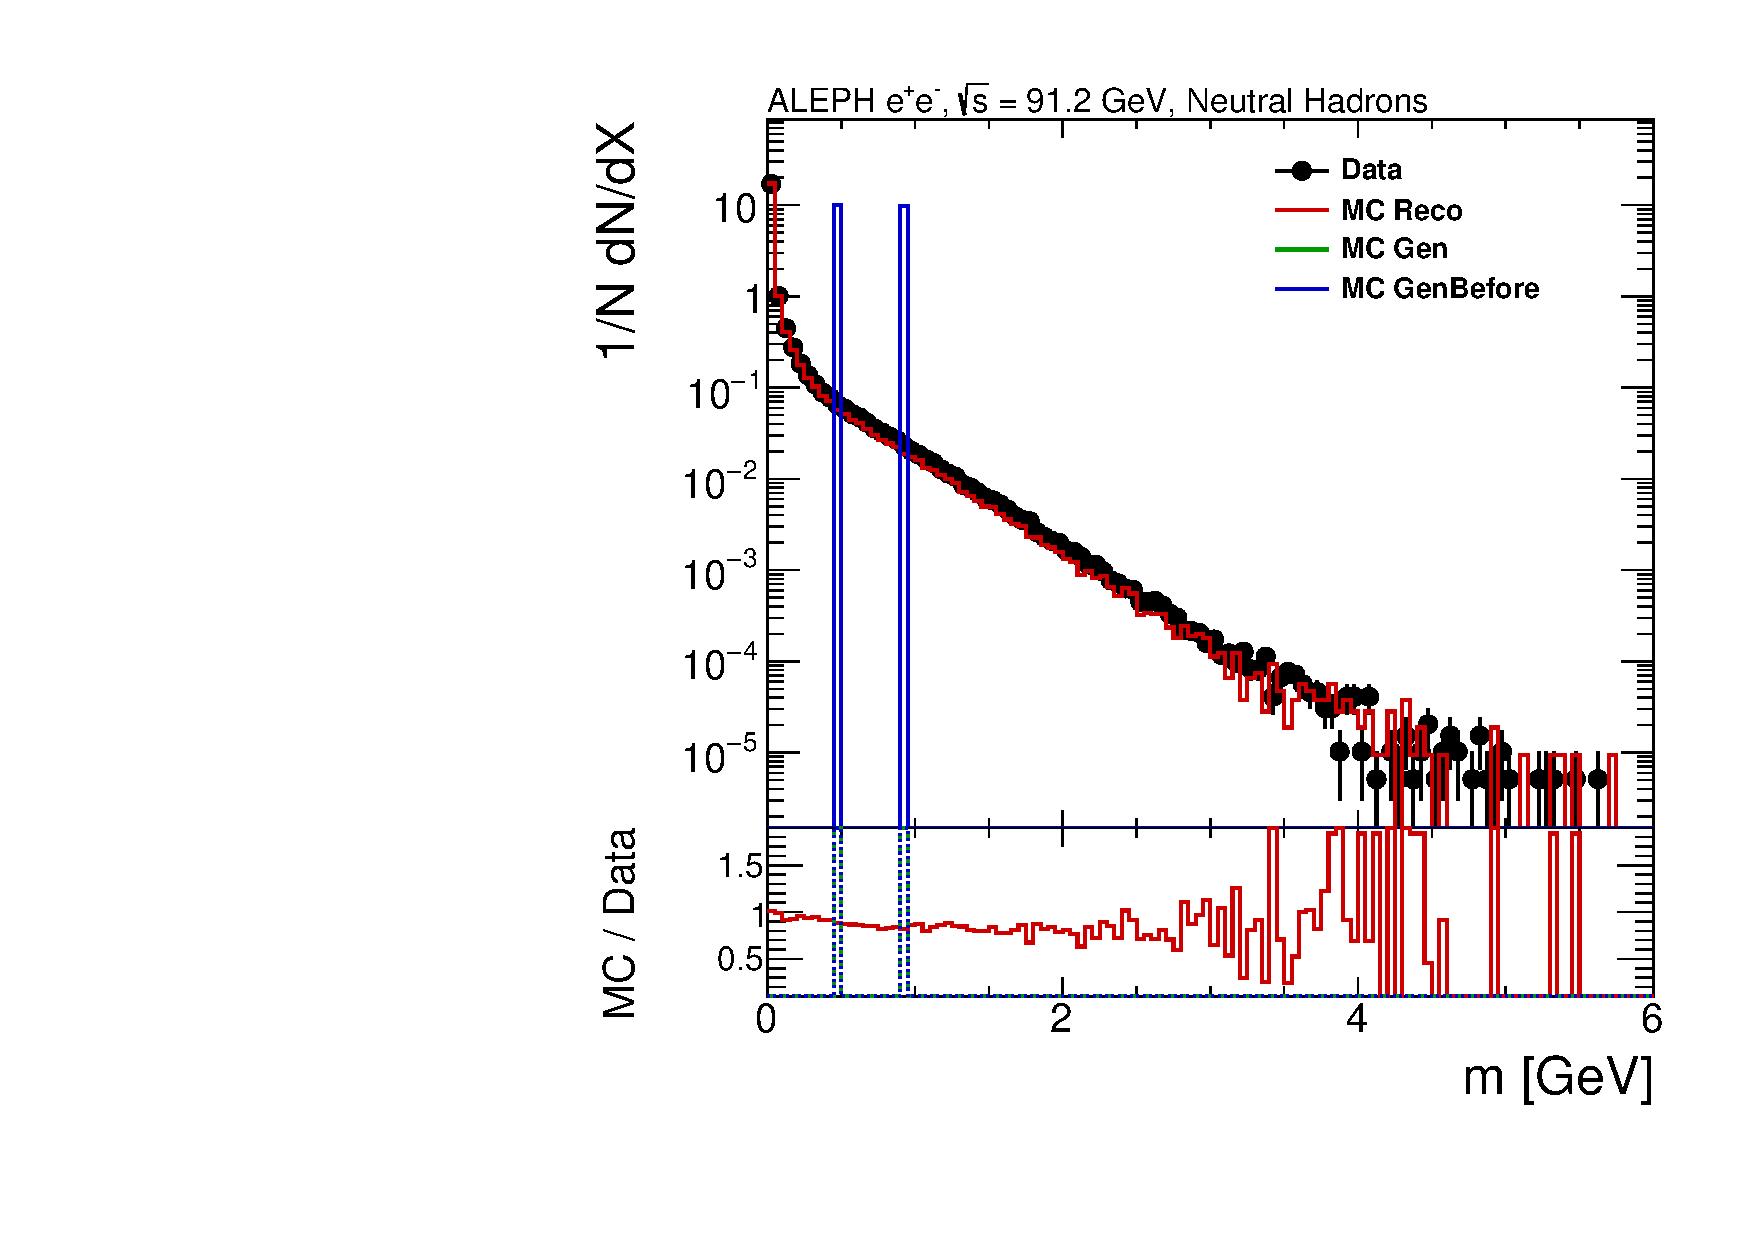
\includegraphics[width=0.325\textwidth]{../Studies/PreliminaryResult/2026-02-17_thrust_iter5/pwflag_kinematics/pwflag5_mass.pdf}
\caption{Complete \texttt{pwflag}=5 kinematic set.}
\label{fig:pwflag5_full}
\end{figure}

\noindent
Figure~\ref{fig:pwflag5_full} completes the neutral-hadron validation; this category is a key
input for neutral-response systematics propagated to the unfolded thrust result. This category is
typically softer and more sensitive to HCAL response and acceptance boundaries, so it is a direct
stress test of the neutral part of the thrust model. The remaining differences in low-statistics
tails are propagated through dedicated neutral-response and cross-check branches in the
experimental systematic program, rather than absorbed into ad hoc selections.


Figure~\ref{fig:pwflag0_full} is the dominant detector-modeling anchor for this analysis because
\texttt{pwflag}=0 tracks provide most of the selected-particle multiplicity and momentum flow. In
this figure, the $\cos\theta$ panel tests geometric acceptance transfer, the impact-parameter
panels test the track-origin and quality region enforced by nominal selections, and the
$N_{\mathrm{TPC}}$ distribution tests detailed tracking response. The $p_T$ and energy spectra are
particularly relevant for thrust because hard tracks can move events across bins near the two-jet
endpoint.

Figures~\ref{fig:pwflag1_full} and~\ref{fig:pwflag2_full} probe the two charged-lepton categories.
Although lower-rate than charged tracks, these objects are important in events with isolated hard
leptons where axis orientation can be sensitive to a small number of particles. Agreement in these
panels demonstrates that category-dependent reconstruction and acceptance do not induce a hidden
bias in thrust inputs.

Figures~\ref{fig:pwflag3_full}--\ref{fig:pwflag5_full} cover $V^0$ candidates, photons, and
neutral hadrons. These categories are essential for total visible energy and hemisphere-sensitive
structure, especially away from the central thrust region. In neutral categories, the angular and
energy spectra are the most important observables because neutral-response mismodeling can directly
alter event-shape normalization and produce larger migration in high-thrust bins. Residual
differences seen in low-statistics tails are propagated via explicit neutral-response systematics
rather than absorbed by additional ad hoc phase-space cuts.

\subsection{Event-level selection observables}

Event-level variables used for hadronic selection are also validated with data/MC comparisons, as shown in Fig.~\ref{fig:event_selection_observables}. These observables summarize the selected particle content and accepted topology that define the phase space used to build detector response and unfolded event-shape spectra.

\begin{figure}[t!]
\centering
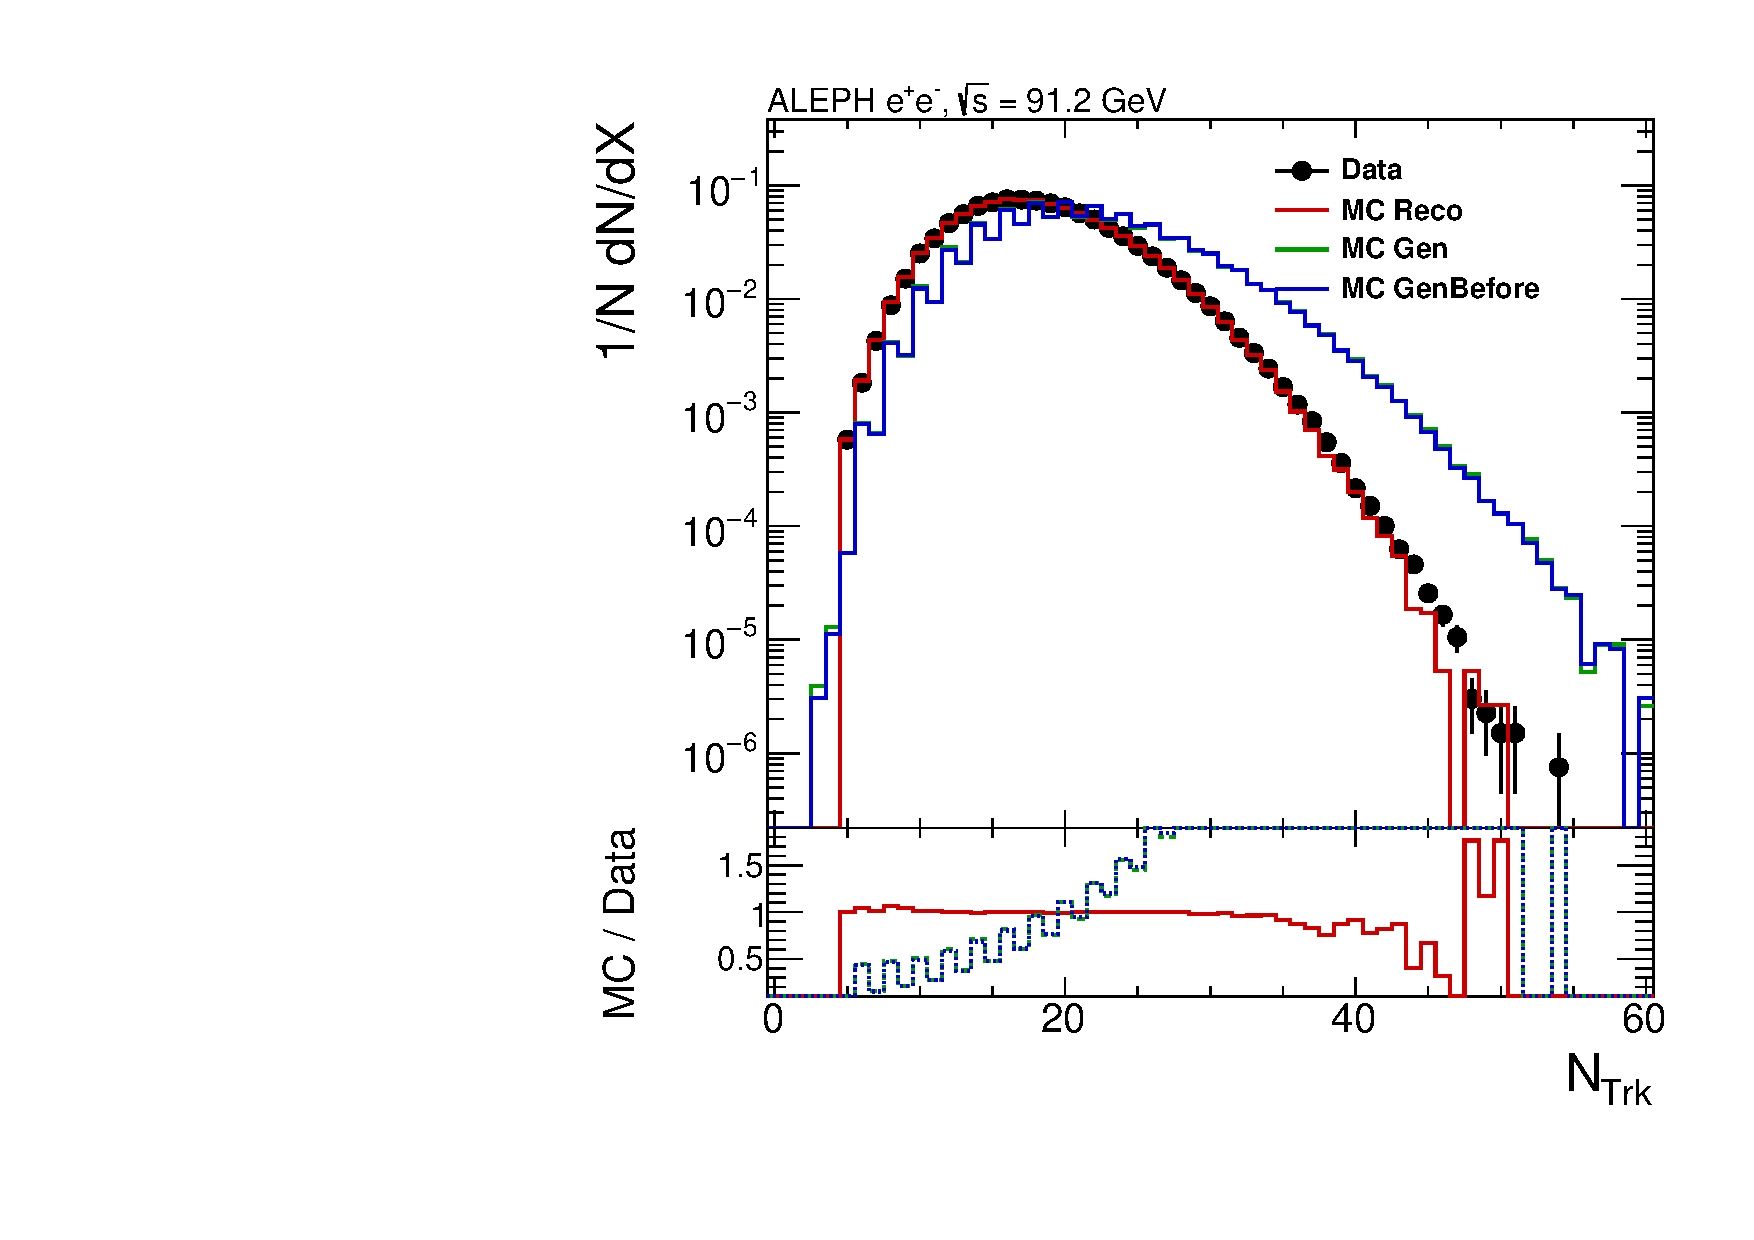
\includegraphics[width=0.495\textwidth]{../Studies/PreliminaryResult/2026-02-17_thrust_iter5/pwflag_kinematics/ntrk.pdf}
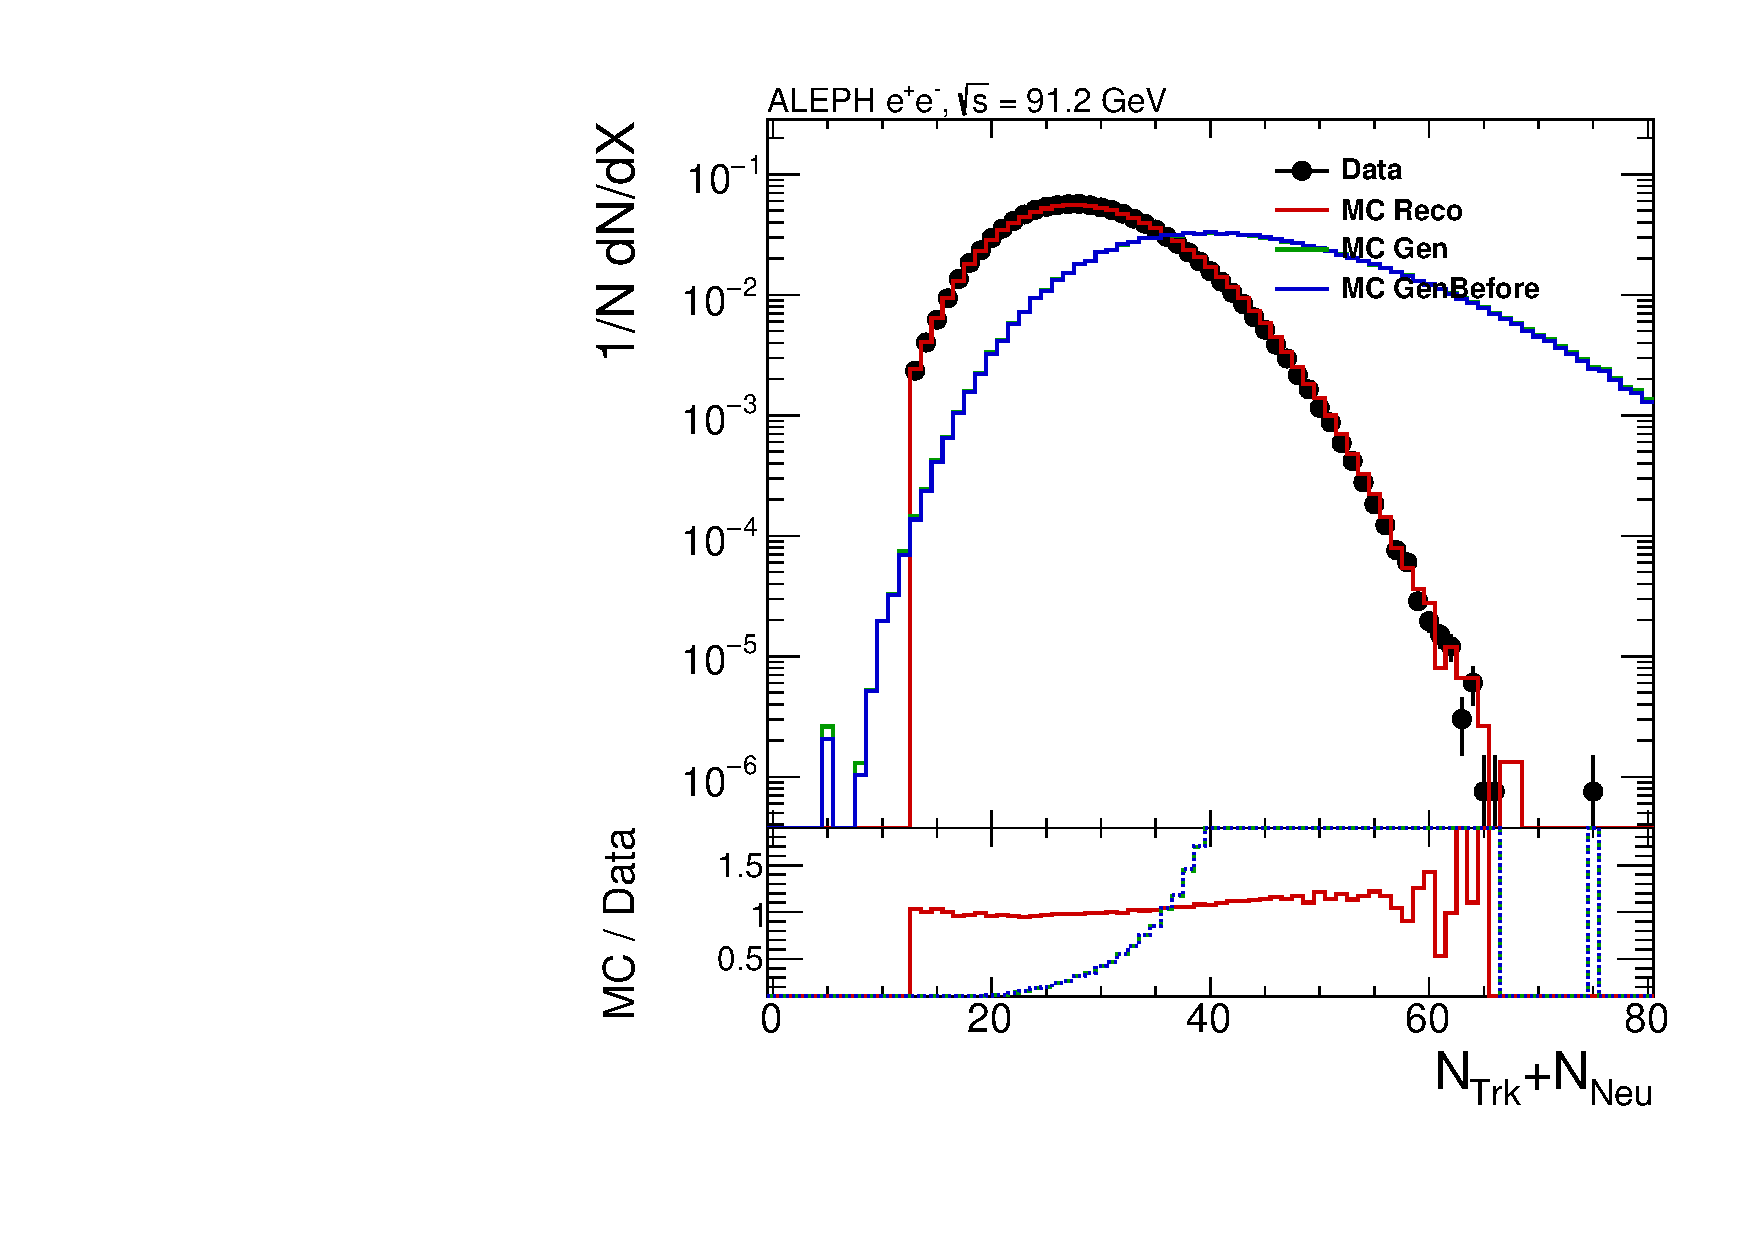
\includegraphics[width=0.495\textwidth]{../Studies/PreliminaryResult/2026-02-17_thrust_iter5/pwflag_kinematics/ntrkPlusNeu.pdf}
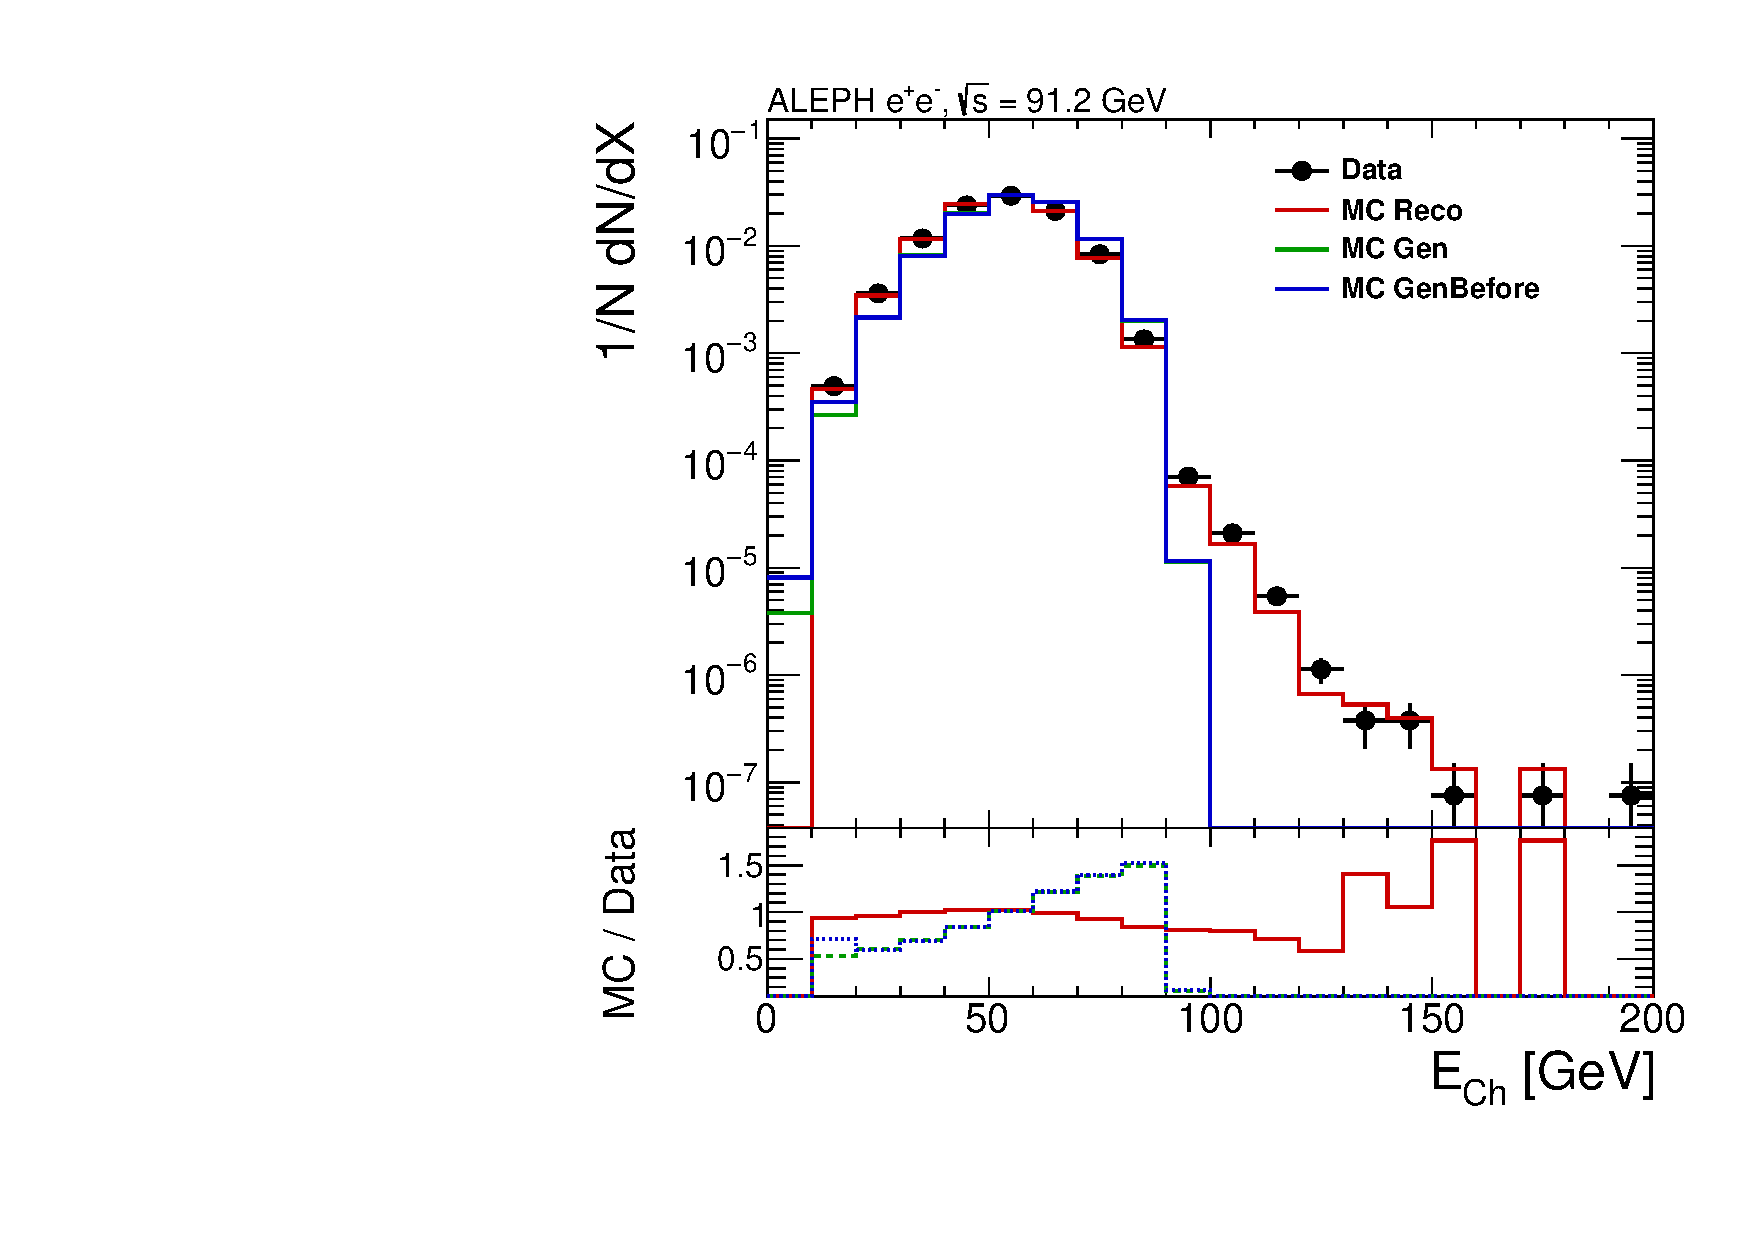
\includegraphics[width=0.495\textwidth]{../Studies/PreliminaryResult/2026-02-17_thrust_iter5/pwflag_kinematics/eCh.pdf}
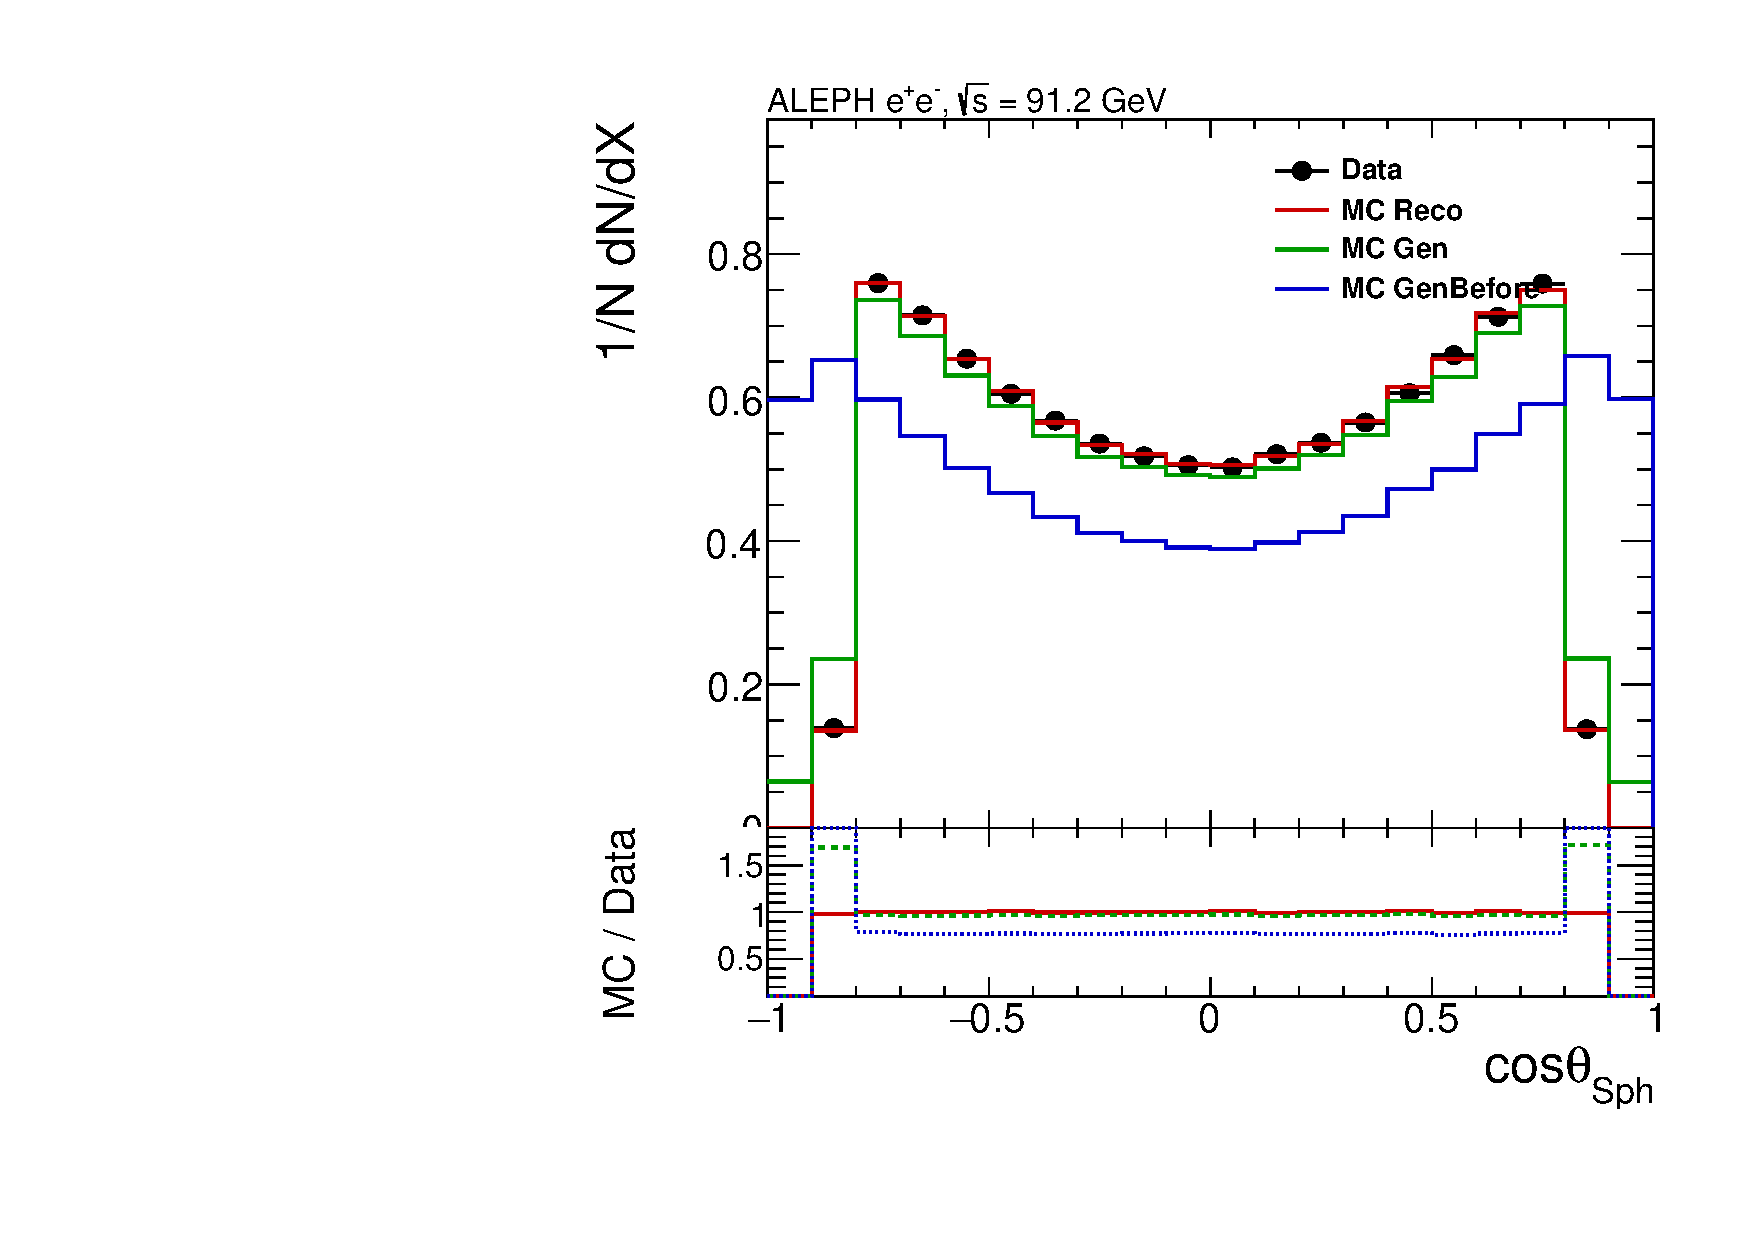
\includegraphics[width=0.495\textwidth]{../Studies/PreliminaryResult/2026-02-17_thrust_iter5/pwflag_kinematics/cosThetaSph.pdf}
\caption{Event-level observables used in the nominal hadronic selection; legends include detector-level data/MC and generator-level references.}
\label{fig:event_selection_observables}
\end{figure}

The event-level panels close the logic between object-level selections and the final sample
entering event-shape reconstruction. $N_{\mathrm{trk}}$ and
$N_{\mathrm{trk}}+N_{\mathrm{neu}}$ test whether multiplicity thresholds sculpt data and MC in a
consistent way; this is critical because those same multiplicities enter hadronic-event
preselection and determine which events contribute to response filling. $E_{\mathrm{Ch}}$ checks
charged-energy modeling near the hadronic-selection boundary at 15 GeV, and
$\cos\theta_{\mathrm{Sph}}$ tests whether accepted event topology is similarly contained in
detector acceptance for data and MC.

Overall agreement in the high-statistics regions supports the response-model baseline used for IBU.
The visible differences are concentrated in lower-populated tails and near selection boundaries,
where statistical fluctuations and detector-response limitations are expected to be larger. These
regions are not ignored: their impact is propagated through the experimental systematic program and
is reflected in the final uncertainty decomposition.

\FloatBarrier
\clearpage
